\documentclass[12pt]{book}
%laatste oefening = nummer 275; 144 mag gebruikt worden.
\usepackage[dutch]{babel}
%\usepackage{amssymb}
%\usepackage{style}
%\hoffset -1.4cm
\setlength{\textwidth}{164mm}
\usepackage{amssymb,amsmath,graphics,graphicx}%,pdfsync}
\usepackage{color}
\usepackage{fancyhdr}
%\usepackage{pslatex}
\usepackage{tikz}
\usepackage[all,cmtip]{xy}
\usetikzlibrary{decorations.markings}
\usepackage[avantgarde]{quotchap} 
\usepackage{appendix,wrapfig}

\definecolor{LGray}{rgb}{0.9,0.9,0.9}

\tikzset{->-/.style={decoration={
  markings,
  mark=at position #1 with {\arrow{>}}},postaction={decorate}}}

\evensidemargin -0cm
\oddsidemargin 0.3cm

\usepackage[colorlinks=false,a4paper,pagebackref]{hyperref}
\renewcommand*{\backreflastsep}{, and }
\renewcommand*{\backreftwosep}{ and }
\renewcommand*{\backref}[1]{}
\renewcommand*{\backrefalt}[4]{ \ifcase #1 \relax \or (on page #2)  \else (on pages #2)  \fi}

%\oddsidemargin 0cm
%\topmargin -1cm
%\textwidth 15.7cm
\textheight 19.87cm
%\parskip 10pt
%\parindent 0pt
%\definecolor{grijs}{rgb}{0.4,0.4,0.4}
%\setlength{\headheight}{15pt}
\fancyhf{}
\renewcommand{\headrulewidth}{0pt}
\fancyhead[LE]{\sffamily\mdseries \thepage~$\mid$ \nouppercase{\leftmark}}
\fancyhead[RO]{\sffamily\mdseries \nouppercase{\rightmark} $\mid$ \thepage}

\fancypagestyle{plain}{
\fancyhf{}
\fancyfoot[LE]{\sffamily\mdseries \thepage~$\mid$}
\fancyfoot[RO]{\sffamily\mdseries $\mid$ \thepage}
\renewcommand{\headrulewidth}{0pt}
\renewcommand{\footrulewidth}{0pt}}


%%\usepackage{mathpple}
%\usepackage{times}
%
%
%
%%\documentclass[12pt]{book}
%%\usepackage{color}
%%\usepackage{graphics}
%\usepackage{amssymb}
%\usepackage{latexsym}
%\usepackage[dutch]{babel}
%%\usepackage{a4wide}
%\usepackage{charter}
%\usepackage{epsfig,makeidx}
%\usepackage{hyperref}
%%\parindent=0mm

\parskip\medskipamount
%\oddsidemargin    10mm    \evensidemargin   0mm    \topmargin        0mm
%\textwidth      150 mm   \textheight     210 mm   \parskip=2pt   \parindent=13pt

\newcommand{\R}{\mathbb{R}}
\newcommand{\Z}{\mathbb{Z}}
\newcommand{\N}{\mathbb{N}}
\newcommand{\D}{\mathbb{D}}
\newcommand{\Sf}{\mathbb{S}}
\newcommand{\dd}{\mathsf{d}}

\newcommand{\bew}{{\sc Bewijs: }}
\newcommand{\B}{\rule{1mm}{0mm} \hfill $\Box$ }
\newcommand{\id}{\mbox{id}}
\newcommand{\C}{\mathbb{C}}

\newtheorem{stelh}{$\!\!$}[section]
\newenvironment{stel}{\begin{stelh}{\em {\bf Stelling }}}{\end{stelh}}
\newtheorem{hfdstelh}[stelh]{$\!\!$}
\newenvironment{hfdstel}{\begin{hfdstelh}{\em {\bf Hoofdstelling }}}{\end{hfdstelh}}
\newtheorem{pointh}[stelh]{$\!\!$}
\newenvironment{point}{\begin{pointh}\em }{\end{pointh}}
\newtheorem{punth}{$\!\!$}
\newtheorem{apb}{$\!\!$}
\newenvironment{punt}{\begin{punth}\em }{\end{punth}}
\newenvironment{apenb}{\begin{apb}\em }{\end{apb}}
\newtheorem{vraagh}{$\!\!$}
\newenvironment{vraag}{\begin{vraagh}\em}{\end{vraagh}} \newtheorem{lemh}[stelh]{$\!\!$}
\newenvironment{lem}{\begin{lemh}{\em {\bf Lemma }}}{\end{lemh}}
\newtheorem{gevh}[stelh]{$\!\!$}
\newenvironment{gev}{\begin{gevh}{\em {\bf Gevolg }}}{\end{gevh}}
\newtheorem{eigh}[stelh]{$\!\!$}
\newenvironment{eig}{\begin{eigh}{\em {\bf Lemma }}}{\end{eigh}}
\newtheorem{vbnh}[stelh]{$\!\!$}
\newtheorem{kons}[stelh]{$\!\!$}
\newenvironment{ekons}{\begin{kons} \em {\bf Constructie }}{\end{kons}}
\newenvironment{vbn}{\begin{vbnh} \em {\bf Voorbeelden.}}{\end{vbnh}}
\newtheorem{vbh}[stelh]{$\!\!$}
\newenvironment{vb}{\begin{vbh} \em {\bf Voorbeeld.} }{\end{vbh}}
\newtheorem{opmh}[stelh]{$\!\!$}
\newenvironment{opm}{\begin{opmh}{\em {\bf Opmerking }}}{\end{opmh}}
\newtheorem{dfh}[stelh]{$\!\!$}
\newenvironment{eopm}{\begin{opmh} \em {\bf Opmerking }}{\end{opmh}}
\newenvironment{df}{\begin{dfh} \em {\bf Definitie }}{\end{dfh}}
%\newtheorem{eoef}[stelh]{$\!\!$}
\newtheorem{eoef}{$\!\!$}[chapter]
\newenvironment{oef}{\begin{eoef} {\bf Oefening}}{\end{eoef}}
\newtheorem{eopl}{$\!\!$}[section]
\newenvironment{opl}{\begin{eopl} \em }{\end{eopl}}
\newtheorem{everm}{$\!\!$}[chapter]
\newenvironment{verm}{\begin{everm} \em }{\end{everm}}
\newenvironment{hint}{{\sc Hint:} }{\\ \rule{1mm}{0mm}
\hfill $\Box$}

\newcommand{\HRule}{\rule{\linewidth}{0.5mm}}

\pagestyle{headings}
\parindent0pt
%%%
\usepackage{amssymb,amsmath}

\begin{document}

\begin{titlepage}
\begin{center}

% Upper part of the page. The '~' is needed because \\
% only works if a paragraph has started.

%
%\textsc{\LARGE University of Beer}\\[1.5cm]
%

% Title
\HRule \\[0.4cm]
{ \huge \bfseries Algebra\"ische topologie en homologe algebra \\[0.4cm] }

\HRule \\[3cm]

\includegraphics[width=0.75\textwidth]{images/outer.jpg}~\\[3cm]


% Author and supervisor
%\noindent
\begin{minipage}{0.4\textwidth}
\begin{flushleft} \large
\large Dr. Koen \textsc{Struyve}
\end{flushleft}
\end{minipage}%
\begin{minipage}{0.4\textwidth}
\begin{flushright} \large
Prof. Dr. Koen \textsc{Thas}
\end{flushright}
\end{minipage}

\vfill

% Bottom of the page
{\large 2014 -- 2015}

\end{center}
\end{titlepage}


%\includegraphics[scale=.3]{outer.jpg}
%\title{\bf ALGEBRAISCHE TOPOLOGIE EN HOMOLOGE ALGEBRA}
%\author{Koen Thas \and Koen Struyve}

% \address{{Universiteit Gent}\\
%{Vakgroep Wiskunde},
%{Krijgslaan 281, S25, B-9000 Gent, Belgi\"{e}}}
%\email{kthas@cage.UGent.be, kstruyve@cage.UGent.be}

%\thanks{The author is a Postdoctoral Fellow
%of the Fund for Scientific Research --- Flanders (Belgium).}
%\date{2013-2014}
%\maketitle
%\hspace*{-20cm}
%\begin{figure}

%\end{figure}


\chapter*{Voorwoord}

De huidige versie van de cursus is gebaseerd op cursusnota's van Prof. Dr. Jan Van Geel, later aangepast door Prof. Dr. Koen Thas. Indien u typ- en/of andere fouten opmerkt gelieve dit door te geven aan de lesgever.


Voorblad: gemerkte metrische grafen vormen een ruimte waarop de uitwendige automorfismegroep van vrije groepen werken, wat het mogelijk maakt deze laatste in detail de bestuderen (naar Karen Vogtmann).
\tableofcontents

\chapter{Begrippen en notaties}
In dit hoofdstuk herhalen we enkele topologische basisbegrippen en notaties die in deze cursus gebruikt zullen worden.

\paragraph{Notaties}
\begin{itemize}
\item Het eenheidsinterval $[0,1]$ met de standaardtopologie noteren we als $I$.
\item $\mathbf{Top}$, de categorie der topologische ruimtes.
\item $\mathbf{Top_*}$, de categorie van gepunte topologische ruimtes, i.e. topologische ruimtes met basispunt.
\end{itemize}


\paragraph{Basisbegrippen}
\begin{itemize}
\item \emph{Aftelbaar van de tweede soort}: Een topologische ruimte is aftelbaar van de tweede soort als de ruimte een aftelbare basis heeft.
\item \emph{Compact}: Een topologische ruimte $X$  is compact als elke overdekking van $X$ met open deelverzamelingen een eindige deeloverdekking bevat. 
\item \emph{Discrete topologie}: Een topologische ruimte $X$ is discreet als elke deelverzameling open is. 
\item \emph{Hausdorff}: Een topologische ruimte $X$ is Hausdorff als voor elke twee verschillende punten $x, y \in X$ er open deelverzamelingen $U,V \subset X$ bestaan zodat $x \in U$, $y \in V$ en $U \cap V = \emptyset$.
\item \emph{Pad-samenhang}: Een topologische ruimte is pad-samenhangend als elke twee punten ervan bevat zijn in een deelruimte homeomorf aan het eenheidsinterval.
\item \emph{Quoti\"enttopologie}: Zij $X$ een topologische ruimte en $\phi: X \to Y$ een surjectieve afbeelding. Een deelruimte $U \subset Y$ is open in de quoti\"enttopologie op $Y$ als het inverse beeld $\phi^{-1}(U)$ open is voor de topologie op $X$. Een veel voorkomende manier om $\phi$ te defini\"eren is aan de hand van een equivalentierelatie.
\item \emph{Samenhang}: Een topologische ruimte is samenhangend als deze niet de disjuncte unie is van twee open deelverzamelingen.
\item \emph{Topologische som}: De topologische som van twee topologische ruimtes $X$ en $Y$ is de topologische ruimte met verzameling punten de disjuncte unie van $X$ en $Y$ en waarbij een verzameling $U$ open is als en slechts als zowel $U \cap X$ en $U \cap Y$ open zijn.
\end{itemize}


\chapter{Vari\"eteiten en CW-complexen}
Vooraleer we algebra\"ische methoden ontwikkelen introduceren we eerst enkele constructiemethodes voor topologische ruimten. Dit zal ons een ruime klasse van voorbeelden opleveren waarop we de technieken van de latere hoofdstukken kunnen toepassen.

Cruciaal hierin is het gebruik van quoti\"entruimtes. 


\section{Topologische vari\"eteiten}

We zullen voornamelijk topologische vari\"eteiten bestuderen. Historisch gezien vormen zij een groot deel van de motivatie voor de ontwikkeling van de algebra\"ische topologie.


\begin{df} 
Een topologische ruimte $X$ is een \emph{$n$-dimensionale (topologische) vari\"eteit} als $X$ Hausdorff is, aftelbaar van de tweede soort, en elk punt $x \in X$ een omgeving heeft die homeomorf is met de Euclidische ruimte $\R^n$ (uitgerust met de standaardtopologie).
\end{df}

\begin{df} 
Een \emph{oppervlak} is een $2$-dimensionale topologische vari\"eteit.
\end{df}


\begin{vb}
De \emph{$n$-sfeer $\mathbb{S}^n$} ($n \geq 1$): dit is de topologische deelruimte 
$$
\{(x_0, x_1, \dots ,x_n ) \in \R^{n+1} \vert x_0^2 + x_1^2 + \dots + x_n^2 = 1 \} 
$$
van de Euclidische ruimte $\R^{n+1}$, en een voorbeeld van een $n$-dimensionale compacte vari\"eteit.
\end{vb}

\begin{vb}
De \emph{$n$-dimensionale torus $\mathbb{T}^n$} ($n \geq 2$): dit is het product 
$$\underbrace{S^1 \times S^1 \times \dots  \times S^1}_n ,$$
uitgerust met de producttopologie.
\end{vb}


\begin{vb}
De \emph{$n$-dimensionale projectieve ruimte $\mathbb{P}^n$} ($n \geq 2$). dit is de quoti\"entruimte van de $n$-sfeer $\mathbb{S}^n$ onder de equivalentierelatie $x \sim -x$ (de antipodale puntenparen worden dus ge\"identificeerd).  
\end{vb}


%\begin{vb}
%De volgende klasse voorbeelden illustreert waarom 3-dimensionale vari\"eteiten een zeer wilde klasse is.
%
%\end{vb}

\section{Vari\"eteiten via triangulaties}
De voorbeelden van vari\"eteiten tot nu toe waren van expliciete aard. Dit zal echter niet altijd handig en/of wenselijk blijken te zijn. Een andere mogelijkheid om  bepaalde vari\"eteiten te construeren is door middel van triangulaties.

\subsection{Trianguleerbare vari\"eteiten}

In de cursus Analyse IV bekwam men de torus $\mathbb{T}^2 := \mathbb{S}^1 \times \mathbb{S}^1$  door in het eenheidsvierkant $I \times I$ de zijdes met dezelfde letter aan elkaar te kleven volgens de ori\"entatie van de pijlen.  
\begin{center}
\begin{tikzpicture}
\fill[fill=LGray] (0,0) -- (2,0) -- (2,2) -- (0,2) -- (0,0);
\draw[->-=.5] (0,0) -- node [below] {$b$} (2,0); 
\draw[->-=.5] (0,2) -- node [above] {$b$} (2,2); 
\draw[->-=.5] (0,0) -- node [left] {$a$} (0,2); 
\draw[->-=.5] (2,0) -- node [right] {$a$} (2,2); 
\end{tikzpicture}
\end{center}

Men kan het voorgaande voorbeeld ook realiseren met behulp van driehoeken als volgt.

\begin{center}
\begin{tikzpicture}
\fill[fill=LGray] (0,0) -- (2,0) -- (2,2);
\fill[fill=LGray] (-1,.6) -- (-1,2.6) -- (1,2.6);

\draw[->-=.5] (0,0) -- node [below] {$b$} (2,0); 
\draw[->-=.5] (2,0) -- node [right] {$a$} (2,2); 
\draw[->-=.5] (0,0) -- node [above left] {$c$} (2,2); 


\draw[->-=.5] (-1,2.6) -- node [above] {$b$} (1,2.6); 
\draw[->-=.5] (-1,.6) -- node [left] {$a$} (-1,2.6); 
\draw[->-=.5] (-1,.6) -- node [below right] {$c$} (1,2.6); 

\end{tikzpicture}
\end{center}

Om deze manier wordt de torus een voorbeeld van een trianguleerbare vari\"eteit. Om deze rigoureus te defini\"eren starten we met simplices.


\begin{df} 
Een $k$-{\em dimensionaal simplex}\index{$k$-dimensionaal simplex} of $k$-{\em simplex}\index{$k$-simplex} $\Delta_{k}$\index{$\Delta_k$} in $\mathbb{R}^{n}$, $k\leq n$, is de 
convex-omhullende $s(e_0, \ldots , e_k)$ van $k + 1$ punten in algemene ligging.
\footnote{De {\em convex-omhullende}\index{convex-omhullende} van $e_0, \ldots , e_k$ is de verzameling 

$$s(e_0, \ldots , e_k)=\{\sum_{i=0}^{k} \lambda_i e_i| 0\leq \lambda_i \leq 1 \mbox{ met } \lambda_0+\cdots +\lambda_k=1\}.$$

De punten $e_0, \ldots , e_k$ zijn in algemene ligging als de vectoren
$(e_1-e_0, \ldots , e_k-e_0)$ lineair onafhankelijk zijn. (De co\"effici\"enten van een punt in $s(e_0, \ldots , e_k)$ zijn uniek.)}
\end{df}

Een $k$-simplex is dus een compacte convexe deelruimte van $\R^k$ waarvan het inwendige niet ledig is, wat impliceert dat een $k$-simplex homeomorf is met de gesloten schijf $\mathbb{D}^{k}$. % (zie pagina 80, Proposition 4.26 in J. Lee, Introduction to Topological Varieties, Springer, 2000).\\

Op deze manier is een 0-simplex is een punt, een 1-simplex een gesloten interval, een 2-simplex een driehoek, een 3-simplex een tetra\"{e}der, enz. 

\begin{df}
Een {\em zijde} van een $k$-simplex opgespannen door $e_0, \ldots , e_k$  is een convex-omhullende van de punten $\{e_0, \ldots , e_{j-1}, e_{j+1}, \ldots , e_k\}$ (we laten dus juist \'e\'en vector weg). 
\end{df}

Een zijde van een $k$-simplex is homeomorf met het standaard $(k-1)$-simplex.




\begin{df}
Een $n$-dimensionale {\em trianguleerbare vari\"eteit} is een topologische vari\"eteit bekomen als quoti\"entruimte door in de topologische som van een mogelijk oneindig aantal $n$-simplices elke zijde met juist \'e\'en andere zijde te identificeren.
\end{df}

In praktijk zullen we onze voorbeelden niet enkel met simplices construeren, we zullen voor de eenvoud ook vaak andere polytopen gebruiken, net zoals we de torus uit een vierkant bekwamen.


\begin{oef}
Ga na dat voor $n=2$ elke quoti\"entruimte die men op deze manier bekomt uit een eindig aantal driehoeken wel degelijk een topologische vari\"eteit is. Zal dit nog steeds het geval zijn voor $n > 2$?
\end{oef}

Men kan zich nu afvragen of elke topologische vari\"eteit trianguleerbaar is. Hoewel dat in het algemeen niet het geval is, is het volgende echter waar.


\begin{stel} \label{stel:triang}
Elke $n$-dimensionale topologische vari\"eteit met $n=2$ of 3, is trianguleerbaar.
\end{stel}
\bew
Zonder bewijs.
\B


\subsection{Oppervlakken}\label{opps}

In deze sectie zullen we de classificatie van de compacte samenhangende oppervlakken schetsen. We starten met twee voorbeelden.


\begin{oef}
Ga na dat quoti\"entruimtes horende bij de volgende triangulaties de sfeer $\mathbb{S}^2$ en het projectief vlak $\mathbb{P}^2$ zijn.

\begin{center}
\begin{tikzpicture}
\fill[fill = LGray] (0,1) circle (1);

\draw[->-=.5] (0,2) arc  (90:-90:1);
\draw (1,1) node [right] {$a$};
\draw[->-=.5] (0,2) arc  (90:270:1);
\draw (-1,1) node [left] {$a$};
\fill (0,0) circle (1.5pt);
\fill (0,2) circle (1.5pt);
\end{tikzpicture}
\hspace{2cm}
\begin{tikzpicture}
\fill[fill = LGray] (0,1) circle (1);

\draw[->-=.5] (0,2) arc  (90:-90:1);
\draw (1,1) node [right] {$a$};
\draw[->-=.5] (0,0) arc  (270:90:1);
\draw (-1,1) node [left] {$a$};
\fill (0,0) circle (1.5pt);
\fill (0,2) circle (1.5pt);
\end{tikzpicture}
\end{center}
\end{oef}

Men kan triangulaties kort en bondig noteren als volgt. Kies een hoekpunt van de polytoop. Doorloop, startend in dit punt, de zijdes van de veelhoek in wijzerzin. Als een zijde in de zelfde ori\"entatie doorlopen wordt noteren we het symbool van deze zijde, anders het symbool met superscript $-1$. Voor de sfeer en het projectief vlak met voorgaande voorstelling bekomen we dus respectievelijk $aa^{-1}$ en $aa$. De torus kan men noteren als $aba^{-1}b^{-1}$.

\begin{oef}
Deze notatie is ver van uniek. Ga na dat de triangulatie $abc a^{-1}b^{-1}c^{-1}$ ook de torus oplevert en dat zowel $abab^{-1}$ als $aabb$ de fles van Klein opleveren.
\end{oef}




We starten met een samenhangend compact oppervlak $S$. Dankzij Stelling~\ref{stel:triang} weten we dat $S$ trianguleerbaar is. Wegens compactheid mogen we veronderstellen dat deze triangulatie bestaat uit een eindig aantal 2-simplices. Het uitwerken van de volgende stappen laten we over als oefening.

\paragraph{Stap a.}
Men kan $S$ bekomen door het lijmen van \'e\'en enkele $2n$-hoek $K$ (waarbij mogelijk is dat $n=1$).
\paragraph{Stap b.}
Indien het aantal hoekpunten van $K$ na identificatie groter is dan 1, dan kan men dit aantal doen verminderen door een paar ge\"identificeerde zijdes te doen krimpen. Dit is altijd mogelijk behalve wanneer $K$ een digon is en $S$ homeomorf is met $\mathbb{S}^2$. We kunnen dus veronderstellen dat het aantal hoekpunten na identificatie 1 is.
\paragraph{Stap c.}
Indien $n \leq 2$, dan is $S$ ofwel een projectief vlak, een torus of een fles van klein. Veronderstel vanaf nu dat $n \geq 3$.
\paragraph{Stap d.}
Een {\em elementaire beweging} in deze context bestaat uit het versnijden van $K$ via een diagonaal die een paar ge\"identificeerde zijdes $e$ en $e'$ scheidt, en het daarna aan elkaar lijmen van de bekomen delen via $e$ en $e'$. Deze operatie be\"invloedt de topologie van $S$ niet.
\paragraph{Stap e.}
Veronderstel dat $x,x'$ en $y,y'$ twee paren ge\"identificeerde zijdes van $K$ zijn die elkaar scheiden. en dat deze gepaard zijn met tegengestelde  ori\"entatie (wijzerzin en tegenwijzerzin ten opzichte van $K$). De resterende zijden van $K$ vormen segmenten  met lengte $m,n,p$ en $q$. Zorg ervoor met behulp van een elementaire beweging dat $m= n=0$. Vind daarna nog een elementaire beweging zodat $m=n=p=0$.
\paragraph{Stap f.}
Indien er geen paren ge\"identificeerde zijdes zijn met gelijke ori\"entatie, dan kan de triangulatie in volgende vorm 
$$
a_1b_1a_1^{-1}b_1^{-1} a_2b_2a_2^{-1}b_2^{-1}  \dots a_gb_ga_g^{-1}b_g^{-1} 
$$
krijgen. Dit stelt een $g$-voudige torus voor. Het getal $g$ noemt men het \emph{genus} van het oppervlak. (Het genus van een sfeer is 0).
\paragraph{Stap g.}
Indien er wel een paar ge\"identificeerde zijdes zijn met gelijke ori\"entatie, dan kan men met behulp van een elementaire beweging bekomen dat er twee adjacente zijdes zijn die ge\"identificeerd worden in gelijke ori\"entatie. 
\paragraph{Stap h.}
De triangulatie $aabbcc$ is homeomorf met de triangulatie $aabcb^{-1}c^{-1}$.
\paragraph{Stap i.}
Indien er een paar ge\"identificeerde zijdes zijn met gelijke ori\"entatie, dan kan de triangulatie in volgende vorm
$$
a_1a_1a_2a_2 \dots a_ga_g
$$
krijgen. Het getal noemt men opnieuw het genus.


Hoewel de classificatie van de compacte samenhangende oppervlakken nu voltooid lijkt, is er echter nog een groot gebrek. We hebben namelijk niet aangetoond dat de bekomen mogelijkheden onderling niet homeomorf zijn. 

Men zal dit pas kunnen doen indien we invarianten aan oppervlakken hechten die behouden worden onder homeomorfismes (Zie Stelling~\ref{klass}). Deze invarianten zullen de homotopie- en homologiegroepen zijn.


\subsection{3-vari\"eteiten}
Hoewel 3--dimensionale topologische vari\"eteiten ook trianguleerbaar zijn, is in tegenstelling tot de oppervlakken er geen eenvoudige aanpak voor deze vari\"eteiten (kortweg \emph{3-vari\"eteiten}) mogelijk.

We schetsen enkele voorbeelden.

\subsubsection{De Poincar\'e dodeca\"edrale ruimte}

De dodeca\"eder is een regelmatig veelvlak met 12 vijfhoeken als zijdes. We lijmen nu paren overstaande zijdes aan elkaar als volgt. De hoekpunten van deze tegenoverliggende zijdes wisselen elkaar af, we moeten dus de zijdes met een hoek draaien. We nemen hiervoor een zijde, we roteren deze 36 graden in wijzerzin, en projecteren deze dan op de overstaande zijde via een translatie. (Zie figuur.) Merk op dat consistent is met de afbeelding van de overstaande zijde op de oorspronkelijke zijde.

\begin{center}
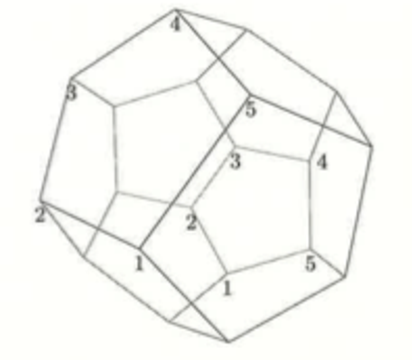
\includegraphics[width=6cm]{images/pds.pdf}
\end{center}

De topologische ruimte die men bekomt noemt men de \emph{Poincar\'e dodeca\"edrale ruimte}.

\begin{oef}
Ga na dat dit een topologische vari\"eteit is.
\end{oef}

\subsubsection{Knopen en 3-vari\"eteiten}

Beschouw de 3-dimensionale torus $\mathbb{T}^3$, deze vari\"eteit is trianguleerbaar en kan men bekomen door in de eenheidskubus $I^3$ de overstaande zijdes aan elkaar te kleven. 

Kies nu een knoop in het inwendige van $I^3$.  Door nu het complement van een dikke gesloten versie $K$ van de knoop in $I^3$ te nemen en daarna de zijdes te identificeren bekomen we een compacte vari\"eteit met rand, waarbij de rand homeomorf is met de 2-dimensionale torus $\mathbb{T}^2$.

We kunnen nu een compacte 3-vari\"eteit construeren door twee op deze manier bekomen compacte vari\"eteiten met rand aan elkaar te kleven via deze rand. Dit levert ons een heel ruime klasse van 3-vari\"eteiten op, wat intu\"itief impliceert dat 3-vari\"eteiten minstens zo complex zijn als knopen.
 
 
\section{CW-complexen}\label{cw}
CW-complexen zijn een klasse van topologische ruimtes die zeer ruim is en die praktisch alle voorbeelden die we zullen behandelen omvat. We  keren terug op het volgende voorbeeld van de torus.

\begin{center}
\begin{tikzpicture}
\fill[fill=LGray] (0,0) -- (2,0) -- (2,2) -- (0,2) -- (0,0);
\draw[->-=.5] (0,0) -- node [below] {$b$} (2,0); 
\draw[->-=.5] (0,2) -- node [above] {$b$} (2,2); 
\draw[->-=.5] (0,0) -- node [left] {$a$} (0,2); 
\draw[->-=.5] (2,0) -- node [right] {$a$} (2,2); 
\end{tikzpicture}
\end{center}


Het inwendige van het vierkant kan men interpreteren als een open schijf, of een \emph{2-cel}, die bevestigd is aan 2 cirkels (de aan elkaar gekleefde zijden $a$ en $b$). Deze twee cirkels kan men ook bekomen door aan hun gemeenschappelijk punt twee open lijnstukken, of twee \emph{1-cellen} te bevestigen. Men kan dus de torus als volgt opbouwen: start met een punt, bevestig twee 1-cellen, en daarna een 2-cel.

Men kan dit proces veralgemenen tot de volgende definitie.
\begin{df} Een \emph{CW-complex} is een topologische ruimte bekomen op de volgende manier.
\begin{enumerate}
\item Start met een discrete verzameling $X^0$, wiens punten we beschouwen als 0-cellen.
\item Inductief construeren we het \emph{$n$-skelet} $X^n$ door aan $X^{n-1}$ $n$-cellen $e
^n_\alpha$ te bevestigen via afbeeldingen $ \phi_\alpha: \mathbb{S}^{n-1} \to X^{n-1}$. We bekomen $X^n$ dus als quoti\"entruimte van de disjuncte unie $X^{n-1} \coprod_\alpha \mathbb{D}^n_\alpha$ van $X^{n-1}$ en een verzameling gesloten $n$-schijven  $\mathbb{D}^n_\alpha$ onder de identificatie $x \sim \phi_\alpha(x)$ met $x\in \partial \mathbb{D}^n_\alpha$. Dus als verzameling $X^n = X^{n-1} \coprod_\alpha e^n_\alpha$ waarbij elke $e^n_\alpha$ een open $n$-schijf is.
\item We herhalen dit inductief een eindig keer, waarbij we dan de uiteindelijke ruimte $X$ gelijk stellen aan de laatste  $n$-skelet $X^n$ die we bekomen hebben. 
\end{enumerate}
\end{df}

De letters C en W staan voor `closure-finiteness' en `weak topology'.


Elke trianguleerbare vari\"eteit is een CW-complex. Alhoewel niet elk CW-complex een topologische vari\"eteit is, en deze definitie momenteel misschien nodeloze complexiteit lijkt, zal dit begrip zeer handig blijken te zijn om homologiegroepen te berekenen.

De klasse van CW-complexen met enkel 0- en 1-cellen, de \emph{grafen}, zullen zeer bruikbaar blijken te zijn in de studie van vrije groepen. 

\section{Lie-groepen}

Als laatste voorbeeld van topologische vari\"eteiten vermelden kort we Lie-groepen. 

\begin{df}
Een \emph{topologische groep} $G$ is een groep met topologische structuur zodanig dat de volgende afbeeldingen continu zijn.
\begin{align*}
G \to G :& g \mapsto g^{-1} \\
G \times G  \to G :& (g,h) \mapsto gh
\end{align*}
\end{df}

\begin{df}
Een \emph{Lie-groep} is een topologische groep die ook een topologische vari\"eteit is.
\end{df}

De theorie van Lie-groepen is sterk ontwikkeld en heeft diepe connecties met differentiaalmeetkunde en algebra\"ische groepentheorie. 

\begin{vbn}
\begin{itemize}
\item De Lie-groep $\mathrm{GL}(n)$, bestaande uit de inverteerbare matrices in $M_{n \times n} (\R)$.
\item De Lie-groep $\mathrm{SL}(n)$, bestaande uit de matrices in $\mathrm{GL}(n)$ met determinant 1.
\item De Lie-groep $\mathrm{SO}(n)$, de deelgroep van $\mathrm{SL}(n)$ die de eenheidssfeer $\mathbb{S}^{n-1}$ in $\R^n$ stabiliseert.
\end{itemize}
\end{vbn}

\begin{oef}
Bepaal de dimensies van deze Lie-groepen als topologische vari\"eteit.
\end{oef}

\begin{oef}
Toon aan dat de Lie-groep $\mathrm{SO}(3)$ homeomorf is met $\mathbb{P}^2$ als topologische ruimte.
\end{oef}




\section{Extra topics}
We vermelden kort enkele onderwerpen als uitbreiding op het voorgaande
 
\subsection{Die Hauptvermutung}

Zoals reeds vermeld zijn niet alle topologische vari\"eteiten trianguleerbaar. Een tweede vraag dat men zich kan stellen is of dat elke twee triangulaties equivalent zijn, i.e. dat ze een gemeenschappelijke deeltriangulatie toelaten. Men kan echter hier een tegenvoorbeeld van vinden geconstrueerd uit de Poincar\'e dodeca\"edrale ruimte.

\begin{df}
Een \emph{suspensie} $SX$ van een topologische ruimte $X$ is de quotientruimte
$$ SX = (X \times I ) / \{(x_1,0 ) \sim (x_2, 0 \} \mbox{ en } (x_1, 1 ) \sim (x_2,1) \mbox{ voor alle } x_1, x_2 \in X \}. $$
\end{df}



\begin{vb}
De suspensie van de sfeer $\mathbb{S}^n$ is $\mathbb{S}^{n+1}$.
\end{vb}

De dubbele suspensie van de Poincar\'e dodeca\"edrale ruimte is homeomorf met de sfeer $\mathbb{S}^5$, maar de triangulatie ge\"induceerd door de suspensies hiervan is echter niet equivalent met een ``standaardtriangulatie" van de sfeer.

\subsection{Vari\"eteiten op abstracte wijze}

Soms willen we extra structuur op een topologische vari\"eteit, zoals ori\"enteerbaarheid, differentieerbaar of gladheid. Op andere momenten zullen we een ruimere klasse, zoals vari\"eteiten met rand bijvoorbeeld, willen beschouwen. Daarom zullen we nu $(G,X)$-vari\"eteiten defini\"eren, wat ons in staat zal stellen om het bovenstaande te realiseren.


\begin{df}
Een \emph{pseudogroep} werkend op een topologische ruimte $X$ is een verzameling $\mathcal{G}$ van homeomorfismes tussen open deelverzamelingen van $X$, zodat de volgende condities voldaan zijn.
\begin{enumerate}
\item De domeinen van de elementen in $\mathcal{G}$ bedekken $X$.
\item De restrictie van een element $g \in \mathcal{G}$ tot een open deelverzameling van het domein van $g$ is opnieuw een element in $\mathcal{G}$.
\item De samenstelling $g_1 \circ g_2$ van twee elementen in $\mathcal{G}$, wanneer gedefinieerd, is opnieuw in $\mathcal{G}$.
\item Het inverse van een element in $\mathcal{G}$ is in $\mathcal{G}$.
\item De eigenschap van een element zijn van $\mathcal{G}$ is {\em lokaal}, d.w.z. indien $g : U \to V$ een homeomorfisme is tussen open verzamelingen van $X$, en $U$ is bedekt door open verzamelingen $U_\alpha$ zodat elke restrictie $g\vert_{U_\alpha}$ in $\mathcal{G}$ is, dan $g \in \mathcal{G}$. 
\end{enumerate}
\end{df}

Uit de definitie volgt dat de identieke afbeelding op elke open verzameling deel uitmaakt van $\mathcal{G}$. De \emph{triviale pseudogroep} is degene die enkel deze afbeeldingen bevat. Aan het andere kant van het spectrum voor de Euclidische ruimte $\R^n$ hebben we dan de pseudogroep $\mathsf{Top}$ die alle homeomorfismes tussen open deelverzamelingen van $\R^n$ bevat.

\begin{df} Zij $\mathcal{G}$ een pseudogroep werkend op een topologische ruimte $X$. Een $(\mathcal{G},X)$-vari\"eteit is een topologische ruimte $M$ met een $(\mathcal{G},X)$-atlas. Een \emph{$(\mathcal{G},X)$-atlas} is een collectie van kaarten $(U_i,\phi_i)$ zodat $\phi_i : U_i \to X$ een homeomorfisme is met $U_i \subset M$ zodat de $U_i$'s open zijn en $M$ bedekken, en zodanig dat elke twee kaarten $(U_i,\phi_i)$ en $(U_j,\phi_j)$ $\mathcal{G}$-compatibel zijn, i.e. 
$$
\gamma_{ij} = \phi_i \circ \phi_j^{-1} : \phi_j(U_i \cap U_j) \to \phi_i(U_i \cap U_j)
$$
is in $\mathcal{G}$.
\end{df}

De topologische $n$-dimensionale vari\"eteiten zijn dus $(\R^n,\mathsf{Top})$-vari\"eteiten. De $(\R^n_+, \mathsf{Top})$-varieteiten zijn nu de vari\"eteiten met rand (waarbij $\R^n_+$ een halfruimte is van $\R^n$). We kunnen ook de pseudogroep $\mathsf{C}^r$ van $\mathcal{C}^r$ diffeomorfismes beschouwen, of de pseudogroep $\mathsf{Top}^+$ bestaande uit de ori\"entatiebewarende homeomorfismes.


\chapter{Homotopie}

Men kan topologische ruimten opvatten als een abstractie van metrische ruimten. Soms is het echter handig om verschillende niet-homeomorfe topologische ruimtes als equivalent te kunnen beschouwen. De volgende drie ruimten zijn bijvoorbeeld niet homeomorf, maar kan men wel ``intu\"itief'' omvormen in elkaar.

\begin{center}
\begin{tikzpicture}
\filldraw[fill=LGray] (0,0) -- (0.5,0) -- (0.5, 1) -- (1.5, 1) -- (1.5,0) -- (2,0) -- (2, 2.5) -- (1.5, 2.5) -- (1.5 , 1.5) -- (0.5 ,1.5) -- (0.5 , 2.5) -- (0, 2.5) -- (0,0);

\draw[style = very thick] (3, 0) -- (3, 2.5)  (3, 1.25) -- (5 , 1.25) (5, 0) -- (5, 2.5) ;

\draw[style = very thick] (6 , 0) -- (8, 2.5) (8, 0) -- (6, 2.5);

\end{tikzpicture}
\end{center}



Om dit rigoureus te  verwezenlijken zullen we homotopie-equivalentie invoeren. 


Deze homotopie-equivalentie zal dan de basis voor het defini\"eren van homotopiegroepen en homologiegroepen  vormen. In het bijzonder zullen deze invariant zijn onder homotopie-equivalentie.

\section{Homotopie}
Stel dat $X,Y$ topologische ruimten zijn en
$f,g:X\to Y$ continue afbeeldingen.

\begin{df}
Een  {\em homotopie}\index{homotopie} van $f$ naar $g$ is een continue afbeelding
$$H:X\times I \to Y$$
zodat
$$H(-,0)=f \mbox{ en } H(-,1)=g$$
met $H(-, t)$ de continue functie $X\to Y; x\to H(x,t)$.

Als er een homotopie tussen $f$ en $g$ bestaat, zeggen we dat $f$ {\em homotoop}\index{homotoop} is met $g$ (in $Y$). We
noteren $f\simeq g$ of $f\simeq_{H} g$.

Een continue afbeelding $f:X\to Y$ noemen we {\em nulhomotoop}\index{nulhomotoop} als $f$ homotoop is met een constante afbeelding.
\end{df}

\begin{eopm}
Een homotopie definieert een 1-parameter familie $h_{t}=H(-,t)$, $0\leq t \leq 1$, van continue
functies van $X\to Y$ met $h_0=f$ en $h_1=g$. 
Intu\"{\i}tief komt een homotopie overeen met een
continue ``deformatie'' van de functie $f$ in de functie $g$.
\end{eopm}

\begin{center}
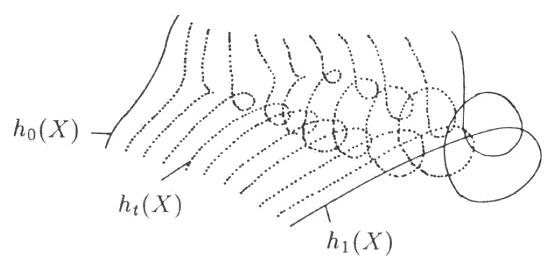
\includegraphics[width=10cm]{images/homotopie.jpg}
\end{center}

\begin{df}
Twee paden $p,q:I\to X$ met vast begin -en eindpunt ($p(0)=q(0)$ en $p(1)=q(1)$) noemen we {\em pad-homotoop}\index{pad-homotoop} (in $X$) als ze homotoop zijn als functies en als de homotopie $H$ zo gekozen kan worden dat voor alle $t\in I$, $p(0)=H(0,t)=h_t(0)=q(0), p(1)=H(1,t)=h_1(1)=q(1).$
\end{df}

%\begin{center}
%\includegraphics[width=6cm]{homotooppad.jpg}
%\end{center}

\begin{eopm}
Homotopie\"en zijn functies van een topologisch product naar een topologische ruimte. Functies $F$ op een product $Y\times Z$ defini\"eren voor elke $y\in Y$, respectievelijk voor elke $z\in Z$, functies $F_y(z):=F((y,z))$ op $Z$, respectievelijk functies $F_z(y):=F((y,z))$ op $Y$. Als $F$ continu is dan zijn ook alle $F_y$ en alle $F_z$ dat. Het omgekeerde is echter niet noodzakelijk waar. 
\end{eopm}

\begin{vbn} \label{vb1deel2} (1) $f:\R \to \R^2: x\mapsto (x,x^2)$ en $g:\R \to \R^2; x\mapsto (x,x)$. De afbeelding
$$H(x,t)=(x,x^2-tx^2+tx)$$
is een homotopie van $f$ naar $g$.\\

(2) Zij $K$ een convex deel van $\R^n$. Zij $f,g:X\to K$ twee continue functies van $X\to K$.
Vermits het lijstuk $[f(x),g(x)]$ volledig in $K$ bevat is ($x \in X$), kunnen we het beeld van $f$
continu deformeren in het beeld van $g$ door langs deze lijnstukken te lopen. De homotopie wordt gegeven door

$$H(x,t)=(1-t)f(x)+tg(x).$$

Deze homotopie noemt men ook de {\em straight-line}\index{straight-line homotopie} homotopie.\\

(3) Door paden te {\em herparametriseren} bekomen we een homotopie van paden. (Deze homotopie\"en zijn handig bij het bestuderen van de fundamentaalgroep, die we verder zullen defini\"eren.)

Een {\em herparametrisatie}\index{herparametrisatie} van een pad $p:I\to X$ is een pad $p\circ \varphi: I\to X$ met $\varphi$ een homeomorfisme $I\to I$ zodat $\varphi(0)=0$ en $\varphi(1)=1$.

Als $F$ een homotopie is tussen de identiteit en $\varphi$, bijvoorbeeld de straight-line homotopie $F(s,t)=(1-t)\varphi(s)+ts$, dan is
$p\circ F$ een pad-homotopie tussen $p$ en $p \circ \varphi$.
\end{vbn}

Het zogenaamde {\em pasting lemma} wordt dikwijls gebruikt om homotopie\"en te defini\"eren.

\begin{lem}{\rm [Pasting Lemma]} 
Zij $X$ en $Y$  topologische ruimten en $f_i:A_i\to Y$, $i=1, \ldots , n$, een eindig stel van continue functies 
op gesloten deelruimten $A_i$ van $X$. Onderstel dat $X=\cup_{i=1}^{n} A_i$. Als voor alle $i, j\in \{1, \ldots, n\}$ geldt dat
$f_{i} (a)=f_{j}(a)$ voor alle $a\in A_i\cap A_j$, dan is er een unieke continue functie $f$ op $X$ zodat 
$f_{|A_i}=f_i$. \label{pasting}
\end{lem}

\bew De functie 

$$f:X\to Y: a \to f_i(a), \mbox{ als } a\in A_i$$

is goed gedefinieerd en men verifieert eenvoudig dat voor alle gesloten verzamelingen $G$ in $Y$ de verzameling $f^{-1}(G)$ gesloten is in $X$. \B


\begin{lem} De relatie $f\simeq g$ is een equivalentierelatie (de {\em homotopierelatie}\index{homotopierelatie}) op de
verzameling van alle continue functies tussen de ruimten $X$ en $Y$. De equivalentieklasse van $f$
duiden we aan met $[f]$.

Zij $X$ een topologische ruimte. Op de verzameling van alle paden in $X$ van $x_0$ naar $x_1$ definieert pad-homotopie een equivalentierelatie.
\end{lem}
\bew Zij $f: X\to Y$ een continue functie. 
Dat $f\simeq f$ is evident. 

Zij $g:X\to Y$ een continue functie en $G:X\times I \to Y$ een homotopie tussen $f$ en $g$. Dan is
$F(x,t)=G(x, 1-t)$ een homotopie tussen $g$ en $f$.

Zij $h: X\to Y$ een continue functie en $H:X\times I \to Y$ een homotopie tussen $g$ en $h$; dan is
$$H'(x,t):=\left\{\begin{array}{l} G(x,2t) \mbox{ als } t\in [0, \frac{1}{2}] \\
H(x, 2t-1) \mbox{ als } t\in [\frac{1}{2}, 1]\end{array}\right.,$$
een homotopie tussen $f$ en $h$. (De continu\"{\i}teit van $H'$ volgt uit het pasting lemma.) 

Dat pad-homotopie een equivalentierelatie definieert, volgt op dezelfde manier.  
\B  

\begin{center}
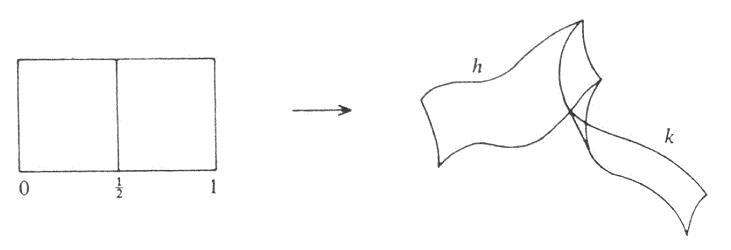
\includegraphics[width=13cm]{images/transitief.jpg}

\vspace{3mm}
{\em Transitiviteit van de homotopierelatie.}
\end{center}

\begin{eig} De homotopierelatie blijft bewaard onder samenstelling van functies; $f_0, g_0:X\to Y$,
$f_0\simeq g_0$ en $f_1, g_1:Y\to Z$, $f_1\simeq g_1$ dan is $f_1\circ f_0\simeq g_1 \circ g_0$.
\end{eig}

\bew De homotopie wordt bepaald door $H_{t}^{(1)}\circ H_{t}^{(0)}$, waarbij $H_{t}^{(0)}$ de homotopie tussen $f_0$ en $g_0$ bepaalt en $H_{t}^{(1)}$ deze tussen $f_1$ en $g_1$. \B

\begin{eig} Zijn $f_i: X_i\to Y_i$ en $g_i:X_i\to Y_i$, voor $i=1,2$ homotope functies, dan is de afbeelding $f_1\times f_2:X_1\times X_2 \to Y_1\times Y_2$ homotoop met de afbeelding $g_1\times g_2:X_1\times X_2 \to Y_1\times Y_2$.
\label{homotopprod}\end{eig}

\bew De homotopie wordt bepaald door $H_{t}^{(1)}\times H_{t}^{(2)}$ waarbij $H_{t}^{(i)}$ de homotopie bepaalt tussen $f_i$ en $g_i$ (voor $i=1,2)$). \B

\begin{df}\label{htop} Een continue afbeelding op een ruimte $X$, $f:X\to X$, noemen we {\em nulhomotoop}\index{nulhomotoop} als $f$ homotoop is met een constante afbeelding. 

Een pad (of lus) $p:I\to X$ met $p(0)=p(1)=x_0$ heet {\em nulhomotoop}\index{nulhomotoop} als $p$ pad-homotoop is met het constante pad $e_{x_{0}}:I \to X: s \mapsto x_0.$  

Zij $X$ en $Y$ topologische ruimten. 
Een continue afbeelding $f:X\to Y$ heet een  {\em homotopie-equivalentie}\index{homotopie-equivalentie} tussen  $X$  en $Y$, als $f$ een  {\em homotoop-inverse}\index{homotoop-inverse} bezit, dit is een continue afbeelding
$g:Y\to X$ zodat $g\circ f\simeq \mbox{id}_{X}$ en $f\circ g\simeq \mbox{id}_{Y}$.

We zeggen dat $X$  {\em homotoop}\index{homotoop} is met $Y$, en noteren $X\simeq Y$,
als er een homotopie-equivalentie tussen $X$ en $Y$ bestaat. 

De categorie van topologische ruimten met als morfismes de homotopieklasses van continue functies noemt men de \emph{homotopiecategorie} en noteert men met $\mathbf{hTop}$. 

Een topologische ruimte $X$ heet  {\em samentrekbaar}\index{samentrekbaar} als $X$ homotoop is met een punt (van $X$).
\end{df} 
\begin{eopm}
Een ruimte $X$ is samentrekbaar als en slechts als er een homotopie $H:X\times [0,1]\to X$ bestaat tussen de identiteit op $X$ en een constante afbeelding $X\to \{p\}\subseteq X$.
Dus $X$ is samentrekbaar als en slechts als de identiteit op $X$ nulhomotoop is.
\end{eopm}

\begin{vb} De ruimte $\R^n$ is samentrekbaar; $H_t:=(1-t)x$ bepaalt een homotopie van $\R^n$ met het nulpunt in $\R^n$.

%\bigskip
%(2) De kegel $CX$ op een topologische ruimte $X$ is samentrekbaar.
%
%De homotopie  $H:(X\times I)\times [0,1]\to X\times I: ((x,s),t)\mapsto (x, 1-(1-s)(1-t))$ samengesteld met de quotientafbeelding induceert een homotopie 
%op het quoti\"ent; $\widetilde{H}: CX\times [0,1] \to CX$. Nu is $\widetilde{H}([(x,s)],0)= (x,s)$ de identiteit op $CX$ en $\widetilde{H}([(x,s)],1)= [(x,1)]$ de constante afbeelding vermits de klasse $[(x, 1)]$ \'e\'en punt voorstelt in $CX$.
%
%\begin{center}
%\includegraphics[width=4cm]{kegel.jpg}
%\end{center}
\end{vb}

\begin{df} Zij $X$ een topologische ruimte en $A$ een deelruimte van $X$.

Een  {\em retract}(ie)\index{retract(ie)} van $X$ op $A$ is een continue afbeelding $r:X\to X$ zodat $r(X)=A$ en
$r_{|A}=\mbox{id}$. We noemen $A$ een {\em retract(ie)}\index{retract(ie)} van X.

Een  {\em deformatie-retract}\index{deformatie-retract} van $X$ op $A$ is een retract $r:X\to A\subseteq X$ die (als afbeelding naar $X$) homotoop is met de identiteit op $X$. We zeggen dat $A$ een  {\em deformatie-retract(ie)}\index{deformatie-retract(ie)} is van $X$.
 
Een  {\em sterk deformatie-retract}\index{sterke deformatie-retract} is een deformatie-retract $r: X\to A\subseteq X$ zodat voor de homotopie $H(x,t)$ tussen $r$ en $\mbox{id}_{X}$ geldt dat $h_t(a)=a$ voor alle $t\in [0,1]$ en alle $a\in A$. (De homotopie houdt de punten van $A$ vast tijdens de deformatie.)
\end{df}

\begin{vbn}
(1) Zij $C$ een gesloten deelruimte van $\R^3$ homeomorf met $\R$. Dan is $C$ een retract van $\R^3$. Dit zien we op de volgende manier. Zij $f:C\to \R$ het homeomorfisme. Tietze 's uitbreidingsstelling geeft een continue afbeelding $f':\R^3\to \R$ zodat $f'_{|C}=f$. Beschouw de afbeelding
$f^{-1}\circ f':\R^3\to C$. Deze afbeelding is continu en beperkt tot $C$ is dit de identiteit. De afbeelding is dus een retract van $\R^3\to C$. 

\bigskip
(2) Het nulpunt is een sterk deformatie-retract van $\R^n$ of van de volle bol $\mathbb{D}^n$. Daaruit volgt dat voor elke topologische ruimte $A$, de ruimte $A\times \{0\}$
een sterke deformatie-retract is van $A\times \R^n$ of van $A\times \mathbb{D}^{n}$.

\begin{center}
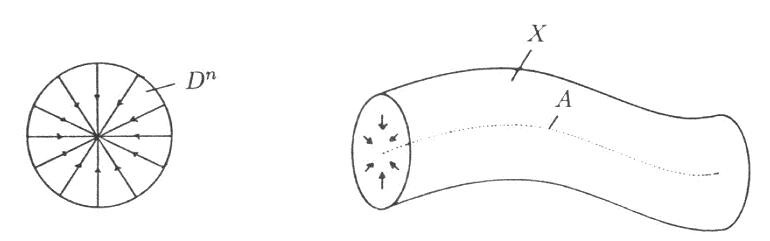
\includegraphics[width=13cm]{images/diskstr.jpg}
\end{center}



(3) Het vorige voorbeeld impliceert dat de volle torus $\mathbb{S}^{1}\times \mathbb{D}^{2}$ homotopie-equivalent is met de cirkel $\mathbb{S}^{1}$.

\begin{center}
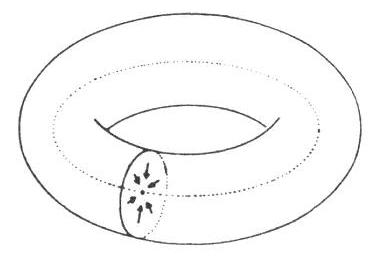
\includegraphics[width=6cm]{images/voltorus.jpg}
\end{center}


%\begin{df} Een  {\em vectorbundel}\index{vectorbundel} $E$ op een topologische ruimte $X$ is een topologische ruimte $E$ met een continue afbeelding $\pi:E\to X$ (de projectie) 
% zodat elke vezel $E_x:=\pi^{-1}(\{x\})$ de structuur heeft van een $\R$-vectorruimte. Verder moet de bundel locaal-triviaal zijn, wat betekent dat er een open overdekking $U_\alpha$ van $X$ bestaat zodat $\pi$ een homeomorfisme $\pi^{-1}(U)\stackrel{\sim}{\to} U\times \R^n$ induceert, waaronder elke vezel $E_x$ lineair-isomorf afgebeeld wordt op $\{x\}\times \R^n$.
%
%Een  {\em snede}\index{snede} van een vectorbundel is een continue afbeelding $\sigma: X\to E$ die elk punt in een element van zijn vezel afbeeldt. De {\em nulsnede}\index{nulsnede} is de snede die elk punt in het nul-element van zijn vezel afbeeldt.
%\end{df}
%
%
%\bigskip
%(4) Zij $E$ een vectorbundel
%op een topologische ruimte $A$, dan is de nulsnede
%een sterk deformatie-retrakt van de bundel $E$ (als topologische ruimte).
%
%\begin{center}
%\includegraphics[width=7cm]{mobiushomtp.jpg}
%\end{center}



(4) De sfeer $\mathbb{S}^{n-1}$ is een sterk deformatie-retrakt van de volle bol min een punt, $\mathbb{D}^{n}\setminus\{0\}$.

\begin{center}
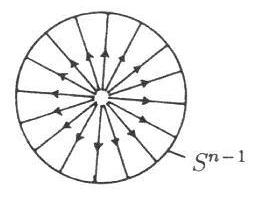
\includegraphics[width=5cm]{images/diskminpt.jpg}
\end{center}

Dit impliceert dat als men aan $X$ een cel kleeft en uit de cel een punt wegneemt, men een ruimte, $X\cup_{\varphi} (\mathbb{D}^{n}\setminus\{0\})$, bekomt die homotoop is met $X$. Namelijk $X\subset X\cup_{\varphi} (\mathbb{D}^{n}\setminus\{0\})$ is een sterk deformatie-retrakt.

\begin{center}
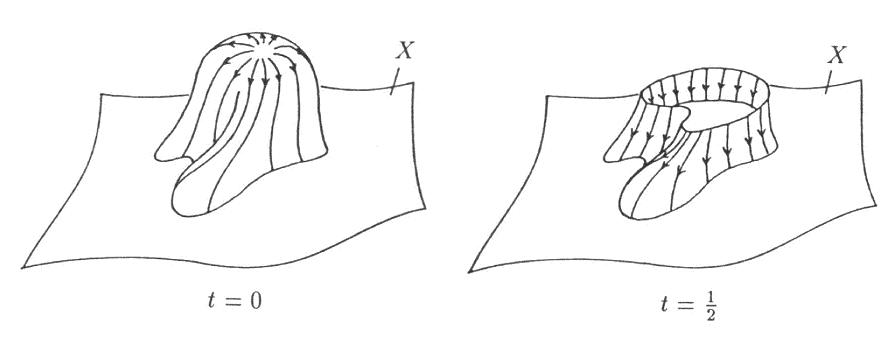
\includegraphics[width=13cm]{images/retrakt.jpg}
\end{center}



(5) 
Zij $0<k<n$ beschouw in $\R^{n+1}\cong \R^{k}\times \R^{n-k+1}$ de sfeer $\mathbb{S}^{n}$.
Het ``sferen-product'' $\frac{\sqrt{2}}{2}(\mathbb{S}^{k-1}\times \mathbb{S}^{n-k}) =\{(x,y)| \ || x ||^{2}=||y ||^{2}=\frac{1}{2}\}$ is een deelruimte van $\mathbb{S}^{n}$.
Deze ruimte is een sterk deformatie retrakt van $\mathbb{S}^{n}\setminus (\mathbb{S}^{k-1}\times \{0\}\cup \{0\}\times \mathbb{S}^{n-k})$.

\begin{center}
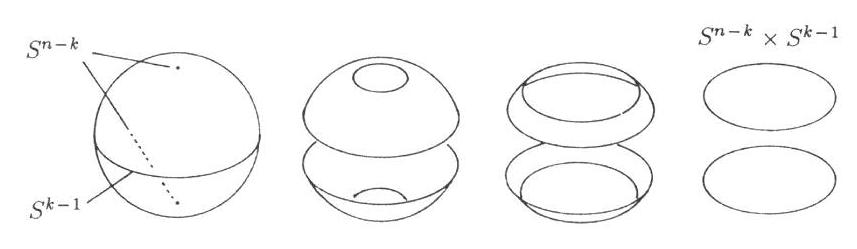
\includegraphics[width=13cm]{images/halfsferen.jpg}
\end{center}


(6)
Een ``acht'' en ``twee cirkels verbonden door een lijn'' zijn homotopie-equivalente ruimten vermits ze beide een sterk deformatie-retrakt zijn van een ``dikke acht''.

\begin{center}
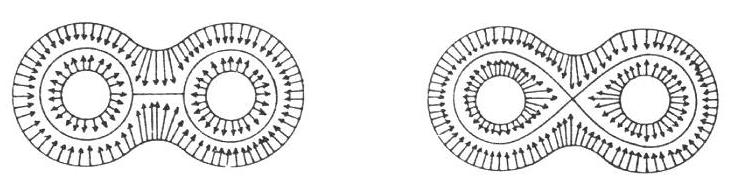
\includegraphics[width=13cm]{images/acht.jpg}
\end{center} 


%(7) Het voorbeeld uit de Morse-theorie. $M_{a}\cup_\varphi \mathbb{D}^{k}$ is een sterk deformatie-retrakt van $M_b$.
%
%\begin{center}
%\includegraphics[width=6cm]{morse2.jpg}
%\end{center}
\end{vbn}
%
\section*{Oefeningen}


\begin{oef} Zij $X$ en $Y$ topologische ruimten. We noteren $[X,Y]$ voor de verzameling van homotopieklassen van continue functies van $X$ naar $Y$.

\begin{itemize}
\item[(a)] Zij $I=[0,1]$. Toon aan dat $[X,I]$ een singelton is.
\item[(b)] Als $Y$ pad-samenhangend is, dan is $[I,Y]$ een singelton.
\end{itemize}
\end{oef}

\begin{oef}
Toon aan dat de retract van een Hausdorff topologische ruimte $X$ gesloten is. (Hint: gebruik dat de diagonaal van $X \times X$ gesloten is.)
\end{oef}

\begin{oef}
Veronderstel dat een punt $x\in X$ een sterk deformatie-retract is van een topologische ruimte $X$, dan bestaat er voor elke omgeving $U$ van $x$ een deelomgeving $x \in V\subset U$ zodanig dat de inclusie $\iota: V \to U$ nulhomotoop is in de deelruimte $U$.
\end{oef}

\begin{oef}
Zij $X$ de deelruimte van het Euclidische vlak $\mathbb{R}^2$ bestaande uit de unie van het horizontaal lijnstuk $[0,1] \times \{0\}$ en de verticale lijnstukken $\{ r\} \times [0,r]$, waarbij $r$ een rationaal getal is in het eenheidinterval.

\begin{center}
\begin{tikzpicture}
\draw[style = semithick] (0,2) -- (0,0)-- (2,0) ;
\foreach \r in {0,...,30}
{
\draw (2-\r/15,0)-- (2-\r/15,\r/15) ;
}
\end{tikzpicture}
\end{center}

Toon dat er een sterk deformatie-retractie bestaat van $X$ naar elk punt van het horizontaal lijnstuk $[0,1] \times \{0\}$, maar niet naar elk ander punt van $X$. 

\end{oef}
%\begin{oef} 
%Voor twee intervallen  $[a,b]$ en $[c,d]$ in $\mathbb{R}$ is er een uniek homeomorfisme van de vorm 
%$\varphi(x)=mx+k$ zodat $\varphi(a)=c$ en $\varphi(b)=d$. (We noemen dit de ``positieve lineair afbeelding'' tussen de intervallen. De graf van deze afbeelding is een rechte met positieve richtingsco\"efficient.) Merk op dat de inverse van dit homeomorfisme ook door een positieve lineaire afbeelding gegeven wordt. Hetzelfde geldt voor de samenstelling van twee positieve lineaire afbeeldingen.
%
%Als $f_1$ en $f_2$ twee paden zijn, dan is $f_3$ (met $[f_1][f_2]=[f_3]$) niets anders dan de afbeelding die op het interval $[0,\frac{1}{2}]$ gelijk is aan de positieve lineaire afbeelding van $[0,\frac{1}{2}]$ naar $[0,1]$, samengesteld met $f_1$, en op het interval $[\frac{1}{2}, 1]$ is het de positieve lineaire afbeelding van $[\frac{1}{2}, 1]$ naar $[0,1]$ samengesteld met $f_2$.
%
%Kies $0<a<b<1$ en definieer voor drie paden $f,g,h$ in $X$, zodat $f(1)=g(0)$ en $g(1)=h(0)$, het ``product''
%$k_{a,b}:I\to X$ op de volgende manier. Op $[0,a]$ is $k_{a,b}$ gelijk aan de positieve lineaire afbeelding van $[0,a]$ naar $I$ samengesteld met $f$. Op $[a,b]$ is $k_{a,b}$ gelijk aan de positieve lineaire afbeelding van $[a,b]$ naar $I$ samengesteld met $g$, en op $[b,1]$ is $k_{a,b}$ gelijk aan de positieve lineaire afbeelding van $[b,1]$ naar $I$ samengesteld met $h$. 
%
%Toon aan dat als $0<c<d<1$, de paden $k_{a,b}$ en $k_{c,d}$ homotoop zijn. 
%
%Gebruik dit om de associativiteit te bewijzen voor de bewerking van de homotopieklassen van paden.
%\end{oef}
%
%
%\input{oefdeel1}



\section{Samenstelling van paden}

Zij $X$ een topologische ruimte. We defini\"eren de samenstelling van paden in $X$. Een pad $f:I\to X$ met $f(0)=x_0$ en $f(1)=x_1$ en een pad $g:I\to X$ met $g(0)=x_1$ en $g(1)=x_2$ kunnen we ``verbinden'' zodat we een pad bekomen van $x_0$ naar $x_2$. Dit pad defini\"eren we als volgt;
$$f*g:=h, \mbox{ met } \left\{\begin{array}{l}h(s)=f(2s) \mbox{ voor } 0\leq s\leq
\frac{1}{2} \\ h(s)=g(2s-1) \mbox{ voor } \frac{1}{2} \leq s\leq 1.\end{array}\right.$$
Dat $f*g$ een goed gedefinieerde continue afbeelding is, volgt uit de voorwaarden $f(1)=g(0)$ en het pasting lemma~\ref{pasting}. 


\begin{lem}
Deze bewerking induceert een bewerking op de homotopieklasse van de paden in $X$:
$$[f][g]:=[f*g].$$
\end{lem}
\bew
We moeten dus verifi\"eren dat als $f\simeq f'$ en $g\simeq g'$, ook $f*g$ homotoop is met $f'*g'$. Als $F$ een homotopie is tussen de paden $f$ en $f'$ en $G$  een homotopie tussen de paden $g$ en $g'$, dan kunnen we eenvoudig verifi\"{e}ren dat

$$H(s,t):=\left\{\begin{array}{ll}
F(2s,t) & \mbox{ als } 0\leq s \leq \frac{1}{2}\\
G(2s-1,t) & \mbox{ als } \frac{1}{2} \leq s \leq 1
\end{array}\right.$$

een homotopie is tussen $f*g$ en $f'* g'$. 
\B

\begin{lem} \label{funct1} Zij $h:X\to Y$ een continue afbeelding tussen twee topologische ruimten. Zij $f$ en $g$ paden in $X$. 

(1) Dan zijn  $h\circ f$  en $h\circ g$ paden in $Y$. 

(2) Als $H$ een (pad-)homotopie is tussen $f$ en $g$ dan is $h\circ H$ een (pad-)homotopie tussen $h\circ f$  en $h\circ g$.

(3) Als het beginpunt van $g$ samen valt met het eindpunt van $f$, dan is 
$$h\circ(f*g):=(h\circ f)*(h\circ g).$$
\end{lem}
\bew De eerste uitspraak is triviaal. Als daarenboven $f$ en $g$ paden zijn met het zelfde begin -en eindpunt geldt dit ook voor $h\circ f$  en $h\circ g$. 

De afbeelding $h\circ H$ is continu, $h\circ H(x, 0)=h\circ f$ en $h\circ H(x,1)=h\circ g$. Als $H$ een pad-homotopie is (in dit geval is $f(0)=g(0)$ en $f(1)=g(1)$), dan is voor alle $t$,  $h\circ H(0,t)= h(f(0))=h(g(0))$ en 
$h\circ H(1,t)= h(f(1))=h(g(1))$. Dus $h\circ H$ is dan ook een pad-homotopie.

De gelijkheid $h\circ(f*g):=(h\circ f)*(h\circ g)$ volgt eveneens onmiddellijk uit de definitie van de bewerking $*$.
\B
\begin{stel}\label{stel:grp} De bewerking $*$ op de homotopieklassen van paden in $X$ voldoet aan de volgende eigenschappen:

{\rm (1)} De bewerking is associatief: als $[f_1]([f_2][f_3])$ gedefinieerd is, dan ook $([f_1][f_2])[f_3]$ en dan zijn beide
homotopieklassen gelijk.

{\rm (2)} Er is een ``linkse'' en ``rechtse'' identiteit. Zij $x\in X$, en noteer met $e_x$ het constante pad $e_x:I\to X: s\to x$. Zij $f$ een pad in $X$ van $x_0$ naar $x_1$. Dan is

$$[e_{x_{0}}][f]=[f]  \mbox{ en } [f][e_{x_{1}}]=[f].$$

{\rm (3)} Elk pad $f$ in $X$ heeft een invers pad. Zij $\overline{f}$ het pad $\overline{f}(s)= f(1-s)$ dan is
$$[f][\overline{f}]=[e_{x_{0}}] \mbox{ en } [\overline{f}][f]=[e_{x_{1}}].$$
\end{stel}
\bew Punt (1) volgt essentieel uit het feit dat een herparametrisering van een pad een homotoop pad geeft. In Oefening~\ref{oef:ass} wordt dit expliciet uitgewerkt.


Punt (2).
Stel dat $e_0$ het constante pad $I\to \{0\}$ is en $i:I\to I$ de identiteit. De afbeelding $i$ is een pad van $I$ naar $I$. 
Dus $e_0*i$ is ook een pad van $I$ naar $I$. Omdat $I$ convex is, bestaat er een pad-homotopie $G$ in $I$ tussen $i$ en $e_0 * i$. Dan is (zie Lemma~\ref{funct1}) $f\circ G$ een pad-homotopie tussen de paden $f\circ i=f$ en $f\circ (e_0*i)=(f\circ e_0)*(f\circ i)=e_{x_{0}}* f.$ Dus $[e_{x_{0}}][f]=[f]$.

Een volledig analoog argument toont $[f][e_{x_{1}}]=[f]$. (Dit geeft Punt (2)).


Om Punt (3) te verifi\"eren beschouwen we $\overline{i}(s)=1-s$ | het ``inverse'' pad van de identiteit $i:I\to I$.
Dan is  $i * \overline{i}$ een pad in $I$ dat begint en eindigt in $0$. Dus het is pad-homotoop met het constante pad $e_0$ omdat $I$ convex is. Als $H$ een pad-homotopie is tussen $e_0$ en $i * \overline{i}$ dan is $f\circ H$ een pad-homotopie tussen $f\circ e_0=e_{x_{0}}$ en $(f\circ i) * (f\circ \overline{i})=f * \overline{f}.$ Dus $[f][\overline{f}]=[e_{x_{0}}]$. De gelijkheid $[\overline{f}][f]=[e_{x_{1}}]$ volgt volledig analoog.
\B





\begin{oef} \label{oef:ass}
Voor twee intervallen  $[a,b]$ en $[c,d]$ in $\mathbb{R}$ is er een uniek homeomorfisme van de vorm 
$\varphi(x)=mx+k$ zodat $\varphi(a)=c$ en $\varphi(b)=d$. (We noemen dit de ``positieve lineair afbeelding'' tussen de intervallen. De graf van deze afbeelding is een rechte met positieve richtingsco\"efficient.) Merk op dat de inverse van dit homeomorfisme ook door een positieve lineaire afbeelding gegeven wordt. Hetzelfde geldt voor de samenstelling van twee positieve lineaire afbeeldingen.

Als $f_1$ en $f_2$ twee paden zijn, dan is $f_3$ (met $[f_1][f_2]=[f_3]$) niets anders dan de afbeelding die op het interval $[0,\frac{1}{2}]$ gelijk is aan de positieve lineaire afbeelding van $[0,\frac{1}{2}]$ naar $[0,1]$, samengesteld met $f_1$, en op het interval $[\frac{1}{2}, 1]$ is het de positieve lineaire afbeelding van $[\frac{1}{2}, 1]$ naar $[0,1]$ samengesteld met $f_2$.

Kies $0<a<b<1$ en definieer voor drie paden $f,g,h$ in $X$, zodat $f(1)=g(0)$ en $g(1)=h(0)$, het ``product''
$k_{a,b}:I\to X$ op de volgende manier. Op $[0,a]$ is $k_{a,b}$ gelijk aan de positieve lineaire afbeelding van $[0,a]$ naar $I$ samengesteld met $f$. Op $[a,b]$ is $k_{a,b}$ gelijk aan de positieve lineaire afbeelding van $[a,b]$ naar $I$ samengesteld met $g$, en op $[b,1]$ is $k_{a,b}$ gelijk aan de positieve lineaire afbeelding van $[b,1]$ naar $I$ samengesteld met $h$. 

Toon aan dat als $0<c<d<1$, de paden $k_{a,b}$ en $k_{c,d}$ homotoop zijn. 

Gebruik dit om de associativiteit te bewijzen voor de bewerking van de homotopieklassen van paden.
\end{oef}

\section{Fundamentaalgroepen}
Zij $X$ een topologische ruimte. Vaak zullen extra veronderstellen dat $X$ pad-samenhangend is. Dit is logisch  aangezien we praten over paden in $X$ en hun samenstellingen. Indien dit niet het geval zou zijn kan men de pad-samenhangendheidscomponenten van $X$ afzonderlijk beschouwen.

Een verzameling met een parti\"ele binaire functie die voldoet aan de eigenschappen van Stelling~\ref{stel:grp} noemt men een \emph{groepo\"ide}. De groepo\"ide gevormd door paden in $X$ en hun samenstelling noemt men de \emph{fundamentaalgroepo\"ide} $\pi_1(X)$ van $X$.

Aangezien de algebra\"ische structuur van een groepo\"ide enigszins beperkt is, leggen we de volgende restrictie op. Kies een punt $x_0 \in X$. We beschouwen nu de homotopieklassen van lussen met  basispunt $x_0$ in de fundamentaalgroepo\"ide.

$$\pi_{1}(X,x_0)=\{[f]|f \mbox{ een pad in } X \mbox{ met } f(0)=f(1)=x_0\} \subset \pi_1(X)$$

Doordat het begin- en eindpunt altijd hetzelfde punt $x_0$ is, zijn de homotopieklassen altijd samenstelbaar, en is de samenstelling en het nemen van een inverse inwendig op $\pi_{1}(X,x_0)$. Hieruit volgt dat $\pi_1(X,x_0)$ een groep is.


\begin{df}
We noemen $\pi_1(X, x_0)$ de {\em eerste homotopiegroep}\index{eerste homotopiegroep} of {\em fundamentaalgroep}\index{fundamentaalgroep} van $X$ met
basispunt $x_0$. 
\end{df}

Deze definitie van de fundamentaalgroep hangt af van het gekozen basispunt. De isomorfismeklasse van de fundamentaal groep is in het pad-samenhangende geval echter onafhankelijk van het basispunt. 

\begin{lem}\label{pix0-pix1}
Zij $X$ pad-samenhangend, $x_0$ en $x_1$ twee punten in $X$ en $p$ een pad in $X$ met beginpunt $x_0$ en eindpunt $x_1$. Dan is 

$$\begin{array}{rcl}
\hat{p}:\pi_{1}(X,x_0) & \to & \pi_{1}(X,x_1)\\
\rule{0mm}{0mm}[f] & \mapsto & [\overline{p}][f][p]\end{array} 
$$

een isomorfisme van groepen.
\end{lem}

\bew  Dit volgt uit $[f][g] \mapsto [\overline{p}][f][g][p]=[\overline{p}][f][p][\overline{p}][g][p]$, waarbij de gelijkheid volgt uit Stelling~\ref{stel:grp}, punt (3). 

Injectiviteit volgt uit het feit dat er een invers element is voor $[p]$ en $[\overline{p}]$. 

Surjectiviteit volgt vermits voor $[g]\in \pi_{1}(X,x_1)$, het element $[p][g][\overline{p}]$ afgebeeld wordt op $[g]$. 
\B


\begin{oef}
Beschouw de fundamentaalgroep $\pi_1(X,x_0)$. Wat is de deelgroep van de automorfismegroep $\mathrm{Aut}(\pi_1(X,x_0))$ gevormd door de automorfismes bekomen door Lemma~\ref{pix0-pix1} toe te passen op het geval waar $p$ een lus is met basispunt $x_0$.
\end{oef}

\begin{eopm} Het isomorfisme tussen $\pi_{1}(X,x_0)$ en $\pi_{1}(X,x_1)$ hangt af van de keuze van het pad $p$
en is dus niet canonisch. Men kan aantonen dat de keuze enkel afhangt van de homotopieklasse van
$p$. Beter kan men echter niet doen | er is geen canonisch isomorfisme tussen homotopiegroepen met
verschillend basispunt. 

We kunnen dus wel van ``de'' fundamentaalgroep van $X$ spreken maar verwijzen dan enkel naar de isomorfismeklasse van de groep.
\end{eopm}


We hebben in het voorgaande een afbeelding van de klasse van gepunte topologische ruimtes naar de klasse van groepen. We willen deze afbeelding uitbreiden tot een functor van de categorie $\mathbf{Top}_*$ naar de categorie $\mathbf{Grp}$. Zij $X$ en $Y$ topologische ruim\-ten met respectievelijke basispunten $x_0, y_0$, en $h : (X, x_0) \to (Y,y_0)$ een morfisme van $\mathbf{Top}_*$ (dus een continue afbeelding die $x_0$ op $y_0$
afbeeldt). Uit Lemma~\ref{funct1} volgt dat $h$ een groepsmorfisme 

\begin{align*}
\pi_1(h) :\pi_{1}(X,x_0) &\to \pi_{1}(Y,y_0) \\
[f] &\mapsto [h\circ f]
\end{align*}
impliceert. Voor de eenvoud noteert men $\pi_1(h)$ met $h_*$.

\begin{stel} {\rm (Functorialiteit)} \label{functor1} $\pi_1: \mathbf{Top}_* \to \mathbf{Grp}$ is een functor.
\end{stel}
\bew
Zij $(X,x_0)$, $(Y,y_0)$ en $(Z,z_0)$ gepunte topologische ruimten en $h: (X,x_0) \to (Y,y_0)$ en $k : (Y,y_0) \to (Z,z_0)$ morfismes in de categorie $\mathbf{Top}_*$.

We hoeven de volgende twee dingen te controleren:

$$
\pi_1(\id_X) = \id_{\pi_1(X,x_0)}
$$
en
$$\pi_1(k \circ h)= \pi_1(k) \circ \pi_1(h).$$

Het eerste punt volgt rechtstreeks uit de definitie van de fundamentaalgroep, het tweede punt volgt uit de definities en de associativiteit van de samenstelling: 

$$\pi_1(k\circ h)([f])=
[(k\circ h) \circ f]=[k\circ (h\circ f)]=\pi_1(k)[h\circ f] =\pi_1(k) \circ \pi_1(h) ([f]),$$

waarbij $f$ een lus is in $X$ met basispunt $x_0$.
\B

Een direct gevolg is dat homeomorfismen van pad-samenhangende topologische ruimten isomorfismen tussen de fundamentaalgroepen induceren. Niet enkel homeomorfismen induceren isomorfismen tussen de fundamentaalgroepen, ook van twee homotope ruimten zijn de fundamentaalgroepen isomorf (Stelling~\ref{functorophomtop}). 

\begin{lem} \label{functorophomtop1} 
Zij $h,k:X\to Y$ continue afbeeldingen. Zij $h(x_0)=y_0$ en $k(x_0)=y_1$. 
Als $H:X\times I\to Y$ een homotopie is tussen $h$ en $k$,
dan is $p(t):=H(x_0,t)$ een pad van $y_0$ naar $y_1$ in $Y$ zodat $\pi_1(k)=\hat{p}\circ \pi_1(h)$, met $\hat{p}$ de afbeelding gedefinieerd in Lemma~\ref{pix0-pix1}.
\end{lem}

\bew Zij $f:I\to X$ een lus in $X$ met basispunt $x_0$. We moeten aantonen dat

$$\pi_1(k)([f])=\hat{p}(\pi_1(h)([f])).$$

Deze gelijkheid is equivalent met

$$[k\circ f]=[\overline{p}]*[h\circ f]*[p]$$

en met

$$[p]*[k\circ f]=[h\circ f]*[p].$$

We verifi\"eren deze laatste gelijkheid.
Beschouw de lussen 

$$f_0(s)=(f(s),0) \mbox{ en } f_1(s)=(f(s),1)$$

in de ruimte $X\times I$.
 Beschouw het pad $c$ in $X\times I$ dat gegeven wordt door 

$$c(t)=(x_0,t).$$

Dan is $H\circ f_0=h\circ f$, $H\circ f_1=k \circ f$ en $H\circ c = p$. 

Zij $F:I\times I \to X\times I$ de afbeelding $F(s,t)=(f(s), t)$. Beschouw de volgende paden
in $I\times I$ (langs de 4 zijden van $I\times I$ lopen),

$$\beta_0(s)=(s,0), \beta_1(s)=(s,1), \gamma_0(t)=(0,t) \mbox{ en } \gamma_1(t)=(1,t).$$

Dan is $F\circ \beta_0=f_0$, $F\circ \beta_1=f_1$ en $F\circ \gamma_0=F\circ \gamma_1=c$.   

De afbeeldingen $\beta_0 * \gamma_1$ en $\gamma_0 *\beta_1$ bepalen paden in $I\times I$ van $(0,0)$ naar $(1,1)$. Vermits $I\times I$ convex is, is er een pad-homotopie $G$ tussen deze 
paden. Dan is $F\circ G$ een pad-homotopie in $X \times I$ tussen $f_0*c$ en $f* f_1$, en $H\circ (F\circ G)$ is een pad-homotopie in $Y$ tussen

$$(H\circ f_0)*(H\circ c)=(h\circ f)*p $$

en 

$$(H\circ c)*(H\circ f_1)= p*(k\circ f).$$
Dit moesten we bewijzen. \B

 
\begin{gev}
Als $h:X\to Y$ nulhomotoop is,  dan is $h_{*}$ het triviale groepsmorfisme.
\end{gev}
\bew Onmiddellijk uit Lemma~\ref{functorophomtop1} \B


\begin{stel}\label{functorophomtop}
Als $f:X\to Y$ een homotopie equivalentie is en $f(x_0)=y_0$, dan is

$$\pi_1(f):\pi_1(X,x_0) \to \pi_{1}(Y,y_0)$$

een isomorfisme. 
\end{stel}
\bew Zij $g:Y\to X$ een homotopie inverse van $f:X\to Y$. Beschouw de volgende afbeeldingen
$$(X,x_0) \stackrel{f}{\to} (Y, y_0) \stackrel{g}{\to} (X,x_1)\stackrel{f}{\to}(Y,y_1),$$
met $x_1=g(y_0)$ en $y_1=f(x_1).$ Dan corresponderen met deze continue afbeeldingen morfismen
$$\pi_1(X,x_0) \stackrel{f_{x_{0}*}}{\to} \pi_{1}(Y,y_0) \stackrel{g_{*}}{\to}
\pi_1(X,x_1) \stackrel{f_{x_{1}*}}{\to} \pi_{1}(Y,y_1).$$
De hypothese stelt dat $g\circ f$ homotoop is met de identiteit, en dus is 
$g_* \circ f_{x_{0}*}$ een isomorfisme. Analoog is $f_{x_{1}*}\circ g_*$ een isomorfisme. 
Het eerst isomorfisme impliceert dat $g_*$ surjectief is en het tweede impliceert dat $g_*$ injectief is. Het feit dat $g_* \circ f_{x_{0}*}$ een isomorfisme is, impliceert dan ook dat $f_{x_{0}*}=f_*$ een isomorfisme is.
\B


\begin{df} Een
topologische ruimte $X$ heet {\em enkelvoudig samenhangend}\index{enkelvoudig samenhangend} als $X$ pad-samenhangend is en als
$\pi_1(X,x_{0})= \{\id\}$.

(Merk op dat deze definitie niet afhangt van het gekozen basispunt.)
\end{df}

Uit Lemma~\ref{functor1} volgt dat ``enkelvoudig samenhangend'' een topologische eigenschap is.
En Stelling~\ref{functorophomtop} impliceert dat ``enkelvoudig samenhangend zijn'' zelfs enkel afhangt van de homotopieklasse van de ruimte.

\begin{vb} $\R^n$ is enkelvoudig samenhangend. Elk pad $p:I\to \R^n$ met $p(0)=p(1)=0$ is
homotoop met het constante pad $e$. Bijvoorbeeld $H(s,t)=tp(s)$ bepaalt zulk een homotopie.

Dus elke bol in $\R^n$ is ook enkelvoudig samenhangend. Meer algemeen zijn samentrekbare ruimten enkelvoudig samenhangend.

We zullen later aantonen dat sferen $\Sf^n$ met $n >1$ enkelvoudig samenhangend zijn. Het bewijs hiervoor is niet triviaal, denk bijvoorbeeld aan het geval van een ruimtevullend pad.
\end{vb}

\begin{lem} \label{lusinenkelvs} Zij $X$ een enkelvoudig samenhangende ruimte. Dan zijn twee paden $p$ en $q$ in $X$ met hetzelfde beginpunt en hetzelfde eindpunt, dus $p(0)=q(0)$ en $p(1)=q(1)$, pad-homotoop. 
\end{lem}
\bew Neem $x_0=p(0)=q(0)$. De lus $p*\overline{q}$ met basispunt $x_0$ definieert een element in $\pi_1(X, x_0)=\{[e_{x_{0}}]\}$. Dus $p*\overline{q}\simeq e_{x_{0}}$ waaruit $p\simeq q$
volgt vanwege Stelling~\ref{stel:grp}. (Hierbij is de equivalentierelatie de pad-homotopierelatie.)\B


\begin{oef}

Zij $A$ een pad-samenhangende deelruimte van een pad-samenhangende 
ruimte $X$. Zij $r :X\rightarrow A$ een retractie, en $x_0\in A$.

\begin{itemize}
\item
Toon aan dat $r_* : \pi_1 (X, x_0 )  \rightarrow \pi_1 (A, x_0 )$ een surjectief morfisme van groepen is.
\item
Toon aan dat $\iota_* : \pi_1 (A, x_0 )  \rightarrow \pi_1 (X, x_0 )$ een injectief morfisme van groepen is.
\end{itemize}
\end{oef}

\section{Berekenen van fundamentaalgroepen}

Tot dusver hebben we nog geen voorbeelden van fundamentaalgroepen gegeven, behalve de triviale groep. In dit hoofdstuk ontwikkelen we enkele methodes om concreet de fundamentaalgroep te bepalen.

%Alvorens we dit concreet doen, geven we een korte inleiding tot groepen via presentaties en geamalgameerde producten.



\subsection{Overdekkingsruimten}\label{section:overdekking}

De theorie die aan de basis ligt van het bepalen van fundamentaalgroepen is de theorie van de overdekkingsruimten. In het bijzonder zullen we de fundamentaalgroep kunnen bepalen van de cirkel, wat de basis is voor het bepalen van algemene fundamentaalgroepen.


\begin{df} Zij $X, Y$ topologische ruimten. Een continue afbeelding 
$Y\stackrel{f}{\to} X$ heet een (lokaal triviale)  {\em fibratie}\index{fibratie} van $X$ als er een open overdekking $U_{\alpha}$ van $X$ bestaat zodat voor alle $\alpha'$ de ruimte $f^{-1}(U_{\alpha'})$ homeomorf
is met het product $U_\alpha' \times Y_{x_{0}}$, waarbij $Y_{x_{0}}=f^{-1}(x_{0})$ de vezel is van $f$ in een (willekeurig) punt $x_0$ van $U_{\alpha'}$. Verder moet de samenstelling van deze homeomorfismen met de projectie op $U_\alpha'$ gelijk zijn aan de restrictie van $f$ op $f^{-1}(U_{\alpha'})$.

Als $Y\stackrel{f}{\to} X$ een fibratie is van $X$, noemt men $Y$ een {\em gevezelde ruimte}\index{gevezelde ruimte}.
\end{df}

\begin{center}
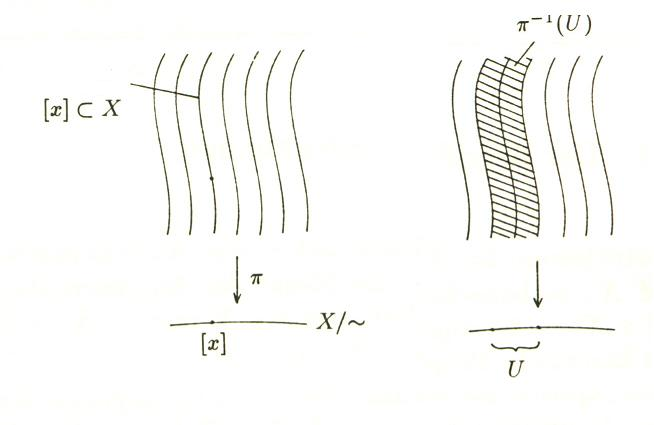
\includegraphics[width=11cm]{images/qrvoor.jpg}
\end{center}



\begin{vbn} (1) Een productruimte $X\times V$ met de projectie $X\times V \to X$ geeft een {\em triviale fibratie}\index{triviale fibratie} van $X$. 

(2) De M\"obiusband is een niet-triviale fibratie van de cirkel.

(3) De Hopf fibraties van $\mathbb{S}^3$ naar $\mathbb{S}^2$. Beschouw het complexe (affiene) vlak $\mathbb{C}^2$, uitgerust met de volgende metriek:
\begin{align*}
\dd : \mathbb{C}^2 \times \mathbb{C}^2 &\to \R \\
(a,b) \times (c,d)  &\mapsto \sqrt{\vert a - c \vert^2 + \vert b- d \vert^2}
\end{align*}
Merk op dat als we $\mathbb{C}^2$ als een vectorruimte over $\R$, dat dit de standaard Euclidische metriek is. De eenheidsbal in het complexe vlak affiene vlak is dus homeomorf met de 3-dimensionale sfeer $\mathbb{S}^3$.

Het complex vlak minus de oorsprong kunnen we continue afbeelden op de projectieve rechte over de complexe getallen. Deze ruimte bestaat uit de complexe getallen (dus een Euclidisch vlak) unie een punt op oneindig, we bekomen dus een 2-dimensionale sfeer $\mathbb{S}^2$. De restrictie van deze afbeelding op $\mathbb{S}^3$ is nu de \emph{Hopf-fibratie} met vezels homeomorf aan $\mathbb{S}^1$. (Men noteert dit soms schematisch met $\Sf^1 \hookrightarrow \Sf^3 \to \Sf^2$.)
\end{vbn}

\begin{eig} Als $X$ een samenhangende ruimte is,  zijn alle vezels van een fibratie van $X$ homeomorf.
\end{eig}
\bew Zij $Y\stackrel{f}{\to} X$ een fibratie van $X$ en $x_0\in X$. We merken eerst op dat alle vezels in punten van een overdekkingsverzameling $U_\alpha$, met $x_0\in U_\alpha$, homeomorf zijn met $Y_{x_{0}}$. Stel nu dat er vezels zijn met een verschillend homeomorfisme type. Beschouw de unie van alle open verzamelingen $U_\alpha$ in de overdekking, waarvoor de vezels van de fibratie van hetzelfde type zijn. Deze unie is een open verzameling en $X$ is de disjuncte unie van zulke open verzamelingen. Als $X$ samenhangend is, kan er dus maar \'e\'en zulke verzameling zijn en dus ook maar \'e\'en homeomorfisme type voor de vezels. \B


\begin{oef}
Men kan ook Hopf-fibraties defini\"eren aan de hand van de quaternionen of de octonionen. Ga na welke ruimtes je krijgt in deze gevallen.
\end{oef}

\begin{df} Onderstel dat $f$ een fibratie $Y\stackrel{f}{\to} X$ is; $Y$ is een  {\em overdekkingsruimte}\index{overdekkingsruimte} (ook kortweg een  {\em overdekking}\index{overdekking} van $X$) als de vezels van deze fibratie discrete ruimten  zijn (verzamelingen met de discrete topologie). 

Als $X$ samenhangend is, zijn de vezels van een overdekking dus discrete ruimten van dezelfde kardinaliteit. Als deze kardinaliteit eindig is | stel gelijk aan $n$ | dan spreken we van een $n$-{\em bladige overdekkingsruimte}\index{$n$-bladige overdekkingsruimte} van $X$.

Als $Y$ een overdekking is van $X$ en $W\subseteq X$ een deelruimte  van $X$, dan is $f^{-1}(W)$ een overdekking van $W$ | we noteren deze met $Y_{|W}$; het is de {\em restrictie} van de overdekkings\-ruimte\index{restrictie} $Y$ tot  $W$.
\end{df}

\begin{vbn} \label{overd} De afbeeldingen
\begin{itemize}
\item $\C\setminus\{0\} \to \C\setminus \{0\}: z\to z^n, n\in \mathbb{N}\setminus\{0\}$;
\item $\C \to \C^{*}: z\mapsto e^{2\pi iz}$;
\item $\R \to\mathbb{S}^{1}= \{z\in \C||z|=1\}: r\mapsto e^{2\pi ir}$;
\item $u:\mathbb{S}^{2}\to \mathbb{P}^{2}$, $u$ de afbeelding die $a$ met $-a$ identificeert;
\end{itemize}
geven voorbeelden van overdekkingsruimten. Het eerste voorbeeld is een $n$-bladige overdek\-kingsruimte, het vierde een tweebladige overdekking.
\end{vbn}

De studie van de overdekkingsruimten van een ruimte $X$ hangt nauw samen met de studie van de fundamentaalgroep van $X$. 
We nemen verder in deze paragraaf {\em steeds aan dat $X$ een pad-samenhangende ruimte is}.

\begin{df} Zij $Y\stackrel{f}{\to} X$ een overdekking en $p:[0,1]\to X$ een pad in $X$. Een pad $\widetilde{p}:[0,1]\to Y$ noemen een  {\em lift}\index{lift} van $p$ als het volgende diagram commuteert.

$$\xymatrix{
I \ar[r]^{\widetilde{p}} \ar[rd]_p & Y \ar[d]^f \\
& X 
}$$


Als $y_0\in Y$ met $f(y_0)=p(0)$ en $\widetilde{p}$ is een lift van $p$ met $\widetilde{p}(0)=y_0$, dan is $\widetilde{p}$ een {\em lift}\index{lift} van $p$ met {\em beginpunt}\index{beginpunt} $y_0$.
\end{df}

\begin{lem} {\rm (Pad-Lifting Lemma)}
Zij $Y\stackrel{f}{\to} X$ een overdekking en $p$ een pad in  $X$. Dan is er voor alle punten $y_0\in f^{-1}(p(0))$ een unieke lift $\widetilde{p}$ van $p$ met beginpunt $y_0$.
\end{lem}

\bew We kiezen een open overdekking $\{U_j\}_{j}$ van $X$ zoals in de definitie van een fibratie. 
We verdelen het interval $I$ in deelintervallen $[s_i, s_{i+1}]$, $i=0, \ldots, n-1$ en $s_0=0, s_n=1$, zodat 
$p([s_i, s_{i+1}])\subset U_{j_{i}}$ voor bepaalde $j_i$. (Dit kan vanwege de compactheid van $I$.)

We defini\"eren de lift $\widetilde{p}$ stap voor stap. We beginnen met $\widetilde{p}(0)=y_0$. Dan onderstellen we dat
$\widetilde{p}(s)$ gedefinie\"erd is voor alle $0\leq s\leq s_i$. Om $\widetilde{p}$ te defini\"eren op $[s_{i}, s_{i+1}]$ merken we op dat $p([s_i, s_{i+1}])$ een deel is van $U_{j_i}$ en dat $f$ een homeomorfisme bepaalt tussen de 
samenhangscomponenten van $f^{-1}(U_{j_{i}})$ en $U_{j_{i}}$. Zij $V_{0}$  de component van $f^{-1}(U_{j_{i}})$
die $\widetilde{p}(s_i)$ bevat. Dan defini\"eren we  voor $s\in [s_i, s_{i+1}]$,
$$\widetilde{p}(s)=(f_{|V_{0}})^{-1}(p(s)).$$
Deze afbeelding (op $[s_i, s_{i+1}]$) is continu omdat $f_{|V_{0}}$ een homeomorfisme is. Op deze manier kunnen we 
$\widetilde{p}$ voor alle $s\in [0,1]$ defini\"eren. Dat we een continue afbeelding bekomen volgt uit het pasting lemma~\ref{pasting}.

We bewijzen nu uniciteit volgt op dezelfde manier, dus door $I$ op te delen in gesloten intervallen en aan te tonen dat twee verschillende lifts identiek zijn op elk interval. \B

Men kan niet enkel paden liften van een ruimte naar een overdekkingsruimte, het volgende zegt dat ook homotopie\"en gelift kunnen worden. 

\begin{lem}
Zij $Y\stackrel{f}{\to} X$ een overdekking. Stel $f(y_0)=x_0$.
Zij $H:I\times I \to X$ een continue afbeelding met $H(0,0)=x_0$. Dan is er een unieke continue lift
$$\widetilde{H}:I\times I\to Y$$
zodat $\widetilde{H}(0,0)= y_{0}$. Als $H$ een homotopie van paden is dan is $\widetilde{H}$ een homotopie van paden.
\label{homotoplift}
\end{lem}

\bew Het bewijs gaat met dezelfde techniek als het bewijs van het pad-lifting lemma, waarbij het eenheidsvierkant opgedeeld wordt in gesloten rechthoeken. \B

\begin{lem} {\rm (Monodromie Lemma)}
Zij $Y\stackrel{f}{\to} X$ een overdekking. Stel $f(y_0)=x_0$.  Zij $p,q$ twee homotope paden in $X$ van $x_0$ naar $x_1$. Zij $\widetilde{p}$ en $\widetilde{q}$ lifts van respectievelijk $p$ en $q$, zodat $\widetilde{p}(0)=\widetilde{q}(0)=y_0$. Dan zijn $\widetilde{p}$ en  $\widetilde{q}$ homotope paden met hetzelfde eindpunt $y_1$ waarvoor geldt $f(y_1)=x_1$.
\end{lem}

\bew Zij $H:I\times I\to X$ de homotopie tussen de paden $p$ en $q$. Dan is $H(0,0)=x_0$. Zij $\widetilde{H}:I\times I \to Y$ de unieke lift van $H$ met $\widetilde{H}(0,0)=y_0$ (Lemma~\ref{homotoplift}). Uit het lemma volgt dat $\widetilde{H}$ een homotopie van paden is, dus $\widetilde{H}(\{0\}\times I)=\{y_0\}$ en $\widetilde{H}(\{1\}\times I)=\{y_1\}$, met $f(y_1)=x_1$. 

De restrictie van $\widetilde{H}$ tot $I\times \{0\}$ is een pad in $Y$ dat begint in $y_0$ en dat het pad 
$H_{| I \times \{0\}}$ lift. De uniciteit van de pad-lifting impliceert dat $\widetilde{H}(s,0)=\widetilde{p}(s)$.
Op dezelfde manier zien we dat $\widetilde{H}(s,1)=\widetilde{q}(s)$. Hieruit volgt dat $\widetilde{H}$ een homotopie is tussen $\widetilde{p}$ en $\widetilde{q}$. Vermits  $\widetilde{H}(\{1\} \times I)=\{y_1\}$ volgt eveneens dat $\widetilde{p}$ en $\widetilde{q}$  hetzelfde eindpunt hebben. \B 

\begin{df} Zij $Y\stackrel{f}{\to} X$ een overdekkingsruimte ($X$ een pad-samenhangende ruimte). Zij $x_0\in X$. De verzameling
$f^{-1}(x_0)$ is een discrete ruimte. Kies $y_0\in Y$ zodat $f(y_0)=x_0$. Voor elk element $[p]\in \pi_{1}(X,x_0)$ noteren we $\widetilde{p}$ voor de unieke lift van $p$ tot $Y$ met 
beginpunt $y_0$. Het monodromie lemma stelt dat

 $$\phi:\pi_1(X,x_0)\to f^{-1}(x_0): [p] \mapsto \widetilde{p}(1)$$
 
een welgedefinieerde afbeelding is. We noemen deze afbeelding (die afhangt van de keuze van het basispunt $x_0$) de  {\em lifting correspondentie}\index{lifting correspondentie} van de overdekking $f:Y\to X$.
\end{df}

\begin{stel} Zij $Y\stackrel{f}{\to} X$ een overdekking. Stel $f(y_0)=x_0$. Als $Y$ pad-samenhangend is dan is de lifting-correspondentie $\phi$ een surjectie. 

Als $Y$ enkelvoudig samenhangend is dan is de lifting-correspondentie $\phi$ een bijectie.
\label{corresp}
\end{stel}
\bew Zij $Y$ pad-samenhangend en $y_1\in f^{-1}(x_0)$. Er is een pad $\widetilde{p}$ in $Y$ van $y_0$ naar $y_1$.  De afbeelding $p=f\circ \widetilde{p}$  is een lus in $X$ met basispunt $x_0$ en per definitie is $\phi([p])=y_1$.

Onderstel nu dat $Y$ enkelvoudig samenhangend is. Zij $[p], [q]$ twee elementen in $\pi_{1}(X,x_0)$ zodat $\phi([p])=\phi([q])$. Zij $\widetilde{p}$, respectievelijk  $\widetilde{q}$, de unieke lift van $p$, respectievelijk van $q$, met beginpunt $y_0$. Dan is $\widetilde{p}(1)=\phi([p])=\phi([q])=\widetilde{q}(1)$. Vermits $Y$ enkelvoudig samenhangend is, bestaat er (vanwege Lemma~\ref{lusinenkelvs}) een homotopie $\widetilde{H}$ in $Y$ tussen $\widetilde{p}$ en $\widetilde{q}$.  De afbeelding $f\circ \widetilde{H}$ is dan een homotopie tussen $p$ en $q$, dus $[p]=[q]$. \B


%Deze enkelvoudig samenhangende overdekkingsruimtes zullen een bijzondere rol spelen in wat komt.

\begin{df} Een overdekking $Y\to X$ heet {\em universeel}\index{universele overdekking} als $Y$ een enkelvoudig sa\-menhangende
ruimte is. 

In de Voorbeelden~\ref{overd} zijn de drie laatste voorbeelden universele overdekkingen. De afbeelding
$$\C^*\to \C^*; z\mapsto z^n$$
is een overdekking die niet universeel is.
\end{df}

Aangezien de sfeer $\Sf^2$ enkelvoudig samenhangend is en we een tweebladige overdekking $u: \Sf^2 \to \mathbb{P}^2$ hebben, volgt hieruit dat de fundamentaalgroep $\pi_1(\mathbb{P}^2, x_0)$ (met $x_0$ in $\mathbb{P}^2$) uit exact twee elementen bestaat. Het kan dus niet anders dan dat deze fundamentaalgroep isomorf is met de cyclische groep op twee elementen.

Tot nu toe kunnen we uit Stelling~\ref{corresp} enkel de kardinaliteit van de de fundamentaalgroep besluiten, de volgende stelling zal ons toelaten om de groep exact te bepalen.


%\bigskip
%De eigenschappen van overdekkingen die we nu bij elkaar hebben laten toe de fundamentaalgroep van het vlak min een punt, $\C^{*}=\C\setminus \{0\}$, te bepalen. Er is namelijk een enkelvoudig samenhangende overdekking van $\C^*$, zijnde $f:\C\to \C^*; z\mapsto e^{2\pi i z}$, waarop we de voorgaande stelling kunnen toepassen. 
%De vezel van deze overdekking in het punt 1, $f^{-1}(1)$, is juist $\Z$. De lifting-correspondentie geeft dan een bijectie tussen $\pi_1(\C^{*}, 1)$ en $\Z$. In de volgende stelling tonen we dat deze bijectie een isomorfisme is.
%
%Vermits $\C\setminus \{0\}$ homotoop is met de cirkel $\mathbb{S}^1$, volgt dat ook 
%$\pi_1(\mathbb{S}^{1}, x_0)\cong \Z.$  (Door de overdekking te beperken tot $\R$ bekomt men een  enkelvoudig samenhangende overdekking van $\mathbb{S}^1$ waaruit men eveneens kan halen dat de fundamentaalgroep van de cirkel isomorf is met $\Z$.) 

\begin{stel}\label{lift2}
Zij $Y\stackrel{f}{\to} X$ een universele overdekking, met $f(y_0) = x_0$. Zij $G$ een groep is die werkt als homeomorfismes op $X$, zodanig dat voor elke $g \in G$ geldt dat $f = f \circ g$,  en zodat $G$ scherp transitief werkt op de vezel $f^{-1}(x_0)$. Dan zijn $G$ en de fundamentaalgroep $\pi_1(X,x_0)$ isomorfe groepen. 
\end{stel}
\bew
De lifting-correspondentie (zie~\ref{corresp}) geeft ons een bijectie van  $\pi_1(X, x_0)$ naar $f^{-1}(x_0)$. Anderzijds hebben we ook de volgende bijectie van $G$ naar $f^{-1}(x_0)$.

$$
g \mapsto g(y_0)
$$

De combinaties van beide bijecties levert ons een bijectie $\alpha$ op van $\pi_1(X,x_0)$ naar $G$. We tonen nu aan dat deze bijectie een isomorfisme van groepen is. Kies lussen $p$ en $q$ in $X$ met basispunt $x_0$. De lifts $\widetilde{p}$ en $\widetilde{q}$ van respectievelijk $p$ en $q$ met basispunt $y_0$ hebben als eindpunt respectievelijk $\alpha([p])(y_0)$ en $\alpha([q])(y_0)$ door de lifting-correspondentie en de definitie van $\alpha$.

Een lift van het samengestelde pad $p * q$ met beginpunt $y_0$ wordt gevormd door het pad $\widetilde{r} :=\widetilde{p} * (\alpha([p]) \circ \widetilde{q})$ wat als eindpunt $\alpha([p]) (\alpha([q])(y_0))$ heeft. Er volgt dus dat 
$$
\alpha([p][q]) = \alpha([p])\alpha([q]) ,
$$
wat impliceert dat $\alpha$ een isomorfisme is. \B



%\begin{stel} \label{fundvlakminpunt} Zij $X=\mathbb{C}\setminus\{0\} = \mathbb{C}^*$ (het re\"{e}el vlak min een punt). Dan is
%$\pi_{1}(X,1)\cong \Z$.
%\end{stel}
%
%
%\bew Beschouw de overdekking
%
%$$f:\mathbb{C} \to \mathbb{C}^{*}; z\mapsto e^{2\pi i z}.$$
%
%De lifting correspondentie hierdoor ge\"{i}nduceerd
%
%$$\phi:\pi_{1}(\C^*, 1)\to \Z$$ 
%
%is een bijectie vanwege de voorgaande stelling. 
%
%We moeten enkel nog aantonen dat $\phi$ een groepsmorfisme is.
%
%Zij $[p]$ en $[q]$ twee elementen in $\pi_1(\C^{*}, 1)$ en $\widetilde{p}, \widetilde{q}$ hun respectievelijke liftings naar $\C$ met beginpunt $0$. Stel $n=\widetilde{p}(1)$ en $m=\widetilde{q}(1)$, dan is $\phi([p])=n$ en $\phi([q])=m$.
%Noteer $\widetilde{\widetilde{q}}$ voor het volgende pad in $\C$
%
%$$\widetilde{\widetilde{q}}(s)=n+\widetilde{q}(s).$$
%
%Omdat $f(n+x)=f(x)$ voor alle $x\in \C$ volgt dat $\widetilde{\widetilde{q}}$ een lift is van $q$ die begint in $n$. 
%De bewerking $\widetilde{p}* \widetilde{\widetilde{q}}$ is gedefinieerd en het is een lift van $p* q$ die begint in $0$. Het eindpunt van dit pad is $\widetilde{\widetilde{q}}(1)=n+m$. Dus per definitie is
%
%$$\phi([p][q])=n+m=\phi([p])+\phi([q]).$$
%
%Vermits $\phi([e_1])=0$ volgt dat de lifting correspondentie dus een isomorfisme van groepen is. \B
De stelling heeft een rist gevolgen.

\begin{gev} \label{fundgrpcirkel} 
De fundamentaalgroep van de cirkel $\mathbb{S}^1$ is
isomorf met $\Z$. \end{gev}
\bew
De overdekking $\R \to\mathbb{S}^{1}= \{z\in \C||z|=1\}: r\mapsto e^{2\pi ir}$ is universeel. De groep $\Z$ werkt op $\R$ via additie en stabiliseert de vezels van de overdekking. \B

%\begin{df} Zij $f:[0,1]\to \C^{*}$ een continue afbeelding, zodat $f(0)=f(1) (= 1)$. Zij
%$W:\pi_{1}(\C^*,1)\to \Z$ het isomorfisme uit Gevolg~\ref{fundgrpcirkel}. Dan noemen we $W(f)$ het
% {\em windingsgetal}\index{windingsgetal} (\emph{omwentelingsgetal, ``winding number''}\index{omwentelingsgetal}\index{winding number})  van $f$.
%\end{df}

\begin{gev}
De fundamentaalgroep van de torus $\mathbb{T}^2$ is isomorf met $\Z^2$.
\end{gev}



\begin{eopm}\label{universal} Indien een ruimte $X$ samenhangend, lokaal pad-samenhangend (elke omgeving van een punt bevat een deelomgeving die pad-samenhangend is) en semi-lokaal enkelvoudig samenhangend (elk punt heeft een omgeving waarvan elke lus samentrekbaar is in $X$) is, dan kan men aantonen dat de universele overdekking bestaat en uniek is op equivariante homeomorfismes na. Ook volgt er het bestaan van een groep $G$ werkend op deze overdekking met de eigenschappen van Stelling~\ref{lift2}. 

De manier om dit te bewijzen is het feit dat er een bijectie is tussen de verzameling van homotopieklassen van paden in $X$ met een vast beginpunt, en de punten van de universele overdekking.
\end{eopm}

We kunnen ook omgekeerd te werk gaan.\label{freeaction} Veronderstel dat $Y$ een enkelvoudige samenhangende ruimte is waarop een groep $G$ van homeomorfismes werkt, zodanig dat er voor elk punt $y \in Y$ een open omgeving $U_y$ van $y$ in $Y$ bestaat zodanig dat alle verzamelingen $g(U_y)$ met $g \in G$ disjunct zijn. In het bijzonder volgt hieruit dat $G$ geen fixpunten heeft op $Y$. 

De quoti\"entafbeelding van $Y$ naar de quotientruimte $X$ bekomen uit $Y$ door de banen van $G$ te identificeren is nu een universele overdekking, met als gevolg dat de fundamentaalgroep van $X$ isomorf is met $G$.


%Wanneer een ruimte een universele overdekkingsruimte heeft, kan men met de redenering uit Stelling~\ref{fundvlakminpunt} van deze ruimte in veel gevallen de fundamentaalgroep bepalen. In zulke gevallen blijkt dat de ruimte een quoti\"entruimte is van de universele overdekkingsruimte, waarbij de equivalentieklassen juist de banen zijn van een actie van de fundamentaalgroep van de basisruimte op de gevezelde ruimte. De fundamentaalgroep bevat dus in die gevallen zeer veel informatie over de ruimte.

Voor de compacte ori\"enteerbare samenhangende oppervlakken van genus $\geq 1$ is het Euclidisch vlak een universele overdekking. Om dit in te zien moeten we in het geval van genus $>1$ wel de hyperbolische metriek op het vlak beschouwen.
Op deze manier bekomt men interessante representaties van de fundamentaalgroep van compacte oppervlakken in $\mathsf{GL}_{2}(\R)$.


\begin{oef}
Toon aan dat de retract van een enkelvoudig samenhangende ruimte een enkelvoudig samenhangende ruimte is.
\item
\begin{itemize}
\item
Toon aan dat er geen retractie van de gesloten schijf naar zijn rand bestaat.
\item
\textbf{(Brouwer fixpuntstelling in dimensie 2)} Toon aan dat elke continue afbeelding van de schijf naar zichzelf een fixpunt heeft.
\end{itemize}

\end{oef}
\begin{oef}
Zij $f : \mathbb{S}^1 \rightarrow \mathbb{S}^1$ een continue afbeelding. Zij $f_* : \pi_1(\mathbb{S}^1,1) \rightarrow \pi_1(\mathbb{S}^1,f(1))$ de geinduceerde afbeelding op de homotopiegroepen. Zij $[\gamma]$ een voortbrenger van  $\pi_1(\mathbb{S}^1,1)$ en $[\gamma']$ een voortbrenger van $ \pi_1(\mathbb{S}^1,f(1))$. We defini\"eren de {\em graad} van $f$ door 
\[
f_*([y]) = \mathrm{deg} f \cdot [\gamma'] .
\] 
Merk op dat dit gedefinieerd is op teken na onafhankelijk van de keuze van voortbrengers.

\begin{enumerate}
\item
Zij $f,g$ twee continue functies van $\mathbb{S}^1$ naar zichzelf. Bepaal $\mathrm{deg} (f \circ g)$.
\item

Toon aan dat als $f$ uitgebreid kan worden tot een continue afbeelding van de gesloten schijf $\mathbb{D}^2$ naar $\mathbb{S}^1$, dat dan de graad van $f$ gelijk is aan nul. 
\item
\textbf{(Lemma van Borsuk)} Zij $f$ een continue afbeelding van $\mathbb{S}^1$ naar zichzelf zodat $f(P^*) =f(P)^*$, waarbij $*$ de antipodale afbeelding is. Toon aan dat de graad van $f$ oneven is. (Hint: gebruik een quoti\"entafbeelding.)
\item
Toon aan dat er geen continue afbeelding bestaat van $\mathbb{S}^2$ naar $\mathbb{S}^1$ zodat $f(P^*) =f(P)^*$.
\item \textbf{(Stelling van Borsuk-Ulam)} 
Zij $f: \mathbb{S}^2 \rightarrow \R^2$ een continue afbeelding. Dan bestaat er een punt $P \in \mathbb{S}^2$ met $f(P)= f(P^*)$.  


\end{enumerate}

\end{oef}
\begin{oef}
Toon aan dat het onmogelijk is de sfeer te overdekken met drie gesloten delen waarvan geen enkel deel een paar antipodale punten bevat.
\end{oef}


\begin{oef}
Veronderstel dat de voorwaarden van Opmerking~\ref{universal} voldaan zijn voor een topologische ruimte $X$. Leg een verband tussen de toevoegingsklassen van deelgroepen van de fundamentaalgroep en de (niet-noodzakelijk universele) samenhangendende overdekkingsruimtes van $X$. Met wat komen de normaaldelers van de fundamentaalgroep overeen?
\end{oef}

\begin{oef}
(Sandwich-stelling). 
Zij $A,B,C$ drie begrensde (samenhangende) volumes in $\R^3$, dan is er er een vlak dat de 3 volumes tegelijk in twee gelijke delen verdeelt.

Hint: De volgende feiten over volumes mag je aannemen:
Zij $l$ een willekeurige lijn in $\R^3$ dan is er een uniek punt zodat het vlak loodrecht op $l$ een gegeven volume $A$ in twee verdeelt. Dit $P_{l,A}$ punt vari\"eert continue als $l$ continue vari\"eert. In het bijzonder:

Stop $A,B,C$ in een grote sfeer $S$ en beschouw voor elk punt $Q$ op de sfeer de lijn $l(Q)$ door $Q$ en $a(Q)$, ($a$ de antipodale afbeelding). Dan is de afbeelding $Q \mapsto P_{l(Q),A}$ een continue afbeelding.

Definieer nu voor elk volume $A,B,C$ de afbeelding
\begin{equation*}
f_X: S \rightarrow \R; Q \mapsto \mbox{ afstand van } Q \mbox{ tot } P_{l(Q),X} \mbox{, met }X \in \{A,B,C\} 
\end{equation*}
Beschouw de afbeelding 
\begin{equation*}
g(Q) = (f_A(Q) - f_C(Q), f_B(Q) - f_C(Q))
\end{equation*}
en pas Borsuk-Ulam toe.
\end{oef}

\subsection{Vrije groepen en geamalgameerde producten}

Een eindig voortgebrachte groep $G$
kan beschreven worden door  {\em generatoren}\index{generatoren en relaties} en  {\em relaties}. Formeel betekent dit dat $G$ gegeven
wordt als de quoti\"entgroep van een vrije groep. Namelijk de eindig voortgebrachte vrije groep voortgebracht door de
generatoren uitgedeeld naar de kleinste normale deelgroep die de relaties ``bevat''.

Als $\{g_1, \ldots , g_n\}$ de verzameling is van de generatoren, dan is een willekeurig element $h$
uit de groep een eindig woord in de symbolen $\{g_1, \ldots , g_n, g_{1}^{-1}, \ldots ,
g_{n}^{-1}\}$. Zulk een woord noemen we {\em gereduceerd}\index{gereduceerd woord} als de symbolen $g$ en $g^{-1}$ niet opeenvolgend
in het woord voorkomen (dus noch $gg^{-1}$, noch $g^{-1}g$ komt voor); het lege woord is dus ook een
gereduceerd woord. De {\em vrije groep}\index{vrije groep} op $n$ generatoren $F=\langle g_1, \ldots , g_n\rangle $ is dan
de groep waarin het lege woord het eenheidselement $\id$ is en waarin de groepswet gegeven wordt door
$ww':=\mbox{red}(ww')$ (met $\mbox{red}(v)$\index{$\mbox{red}(v)$} de reductie van het woord $v$).

Een groep {\em gerepresenteerd door generatoren  en relaties}\index{gerepresenteerd door generatoren  en relaties}, $G=\langle g_1, \ldots , g_n| w_1, \ldots,
w_m\rangle$ met $w_i$ gereduceerde woorden in de $g_{i}$'s, is de quoti\"entgroep van
de vrije groep $F$ voortgebracht door $g_1,\ldots ,g_n$ met de normale deelgroep
$N(\langle w_1,\ldots, w_m\rangle)$.

Het {\em vrij product}\index{vrij product} van twee groepen $G_1\ast G_2$ is de groep die bestaat uit de woorden
van de vorm $v_1\ldots v_s$ met $v_i\in G_1\cup G_2$. Het product van twee woorden $v_1\ldots v_s$, $w_1\ldots
w_r$ is bij definitie $v_1\ldots v_sw_1\ldots w_r$. De groepen $G_1$ en $G_2$ kan men op natuurlijke manier
opvatten als deelgroepen van de groep $G_1\ast G_2$. Men kan het vrije product ook defini\"eren met
een universele of karakteriserende eigenschap.

\begin{stel} Voor elk stel groepsmorfismen $\phi_{1}:
G_1\to E$ en $\phi_{2}:G_2\to E$ is er een uniek groepsmorfisme $\Phi: G_1\ast G_2 \to E$ zodat
$\Phi_{|G_1}=\phi_1$ en $\Phi_{|G_2}=\phi_2$.

Deze eigenschap karakteriseert het vrij product van twee groepen op isomorfisme na.
\end{stel}

Als de groepen $G_1$ en $G_2$ het beeld van een groep $H$ onder groepsmorfismen $\phi_i:H\to
G_i$ bevatten definieert men het  {\em geamalgameerd product}\index{geamalgameerd product} van $G_1$ en $G_2$, notatie
$G_1\ast_{H}G_2$. Het is de quoti\"entgroep $(G_1\ast G_2)/N$ met $N$ de kleinste normale deelgroep
die de elementen $\phi_1(h)\phi_{2}(h)^{-1}$, met $h\in H$, bevat. 


\begin{vb} Zij $G_1=\langle g_1, \ldots, g_n|w_1, \ldots ,w_r\rangle$,
$G_2=\langle g'_1, \ldots, g'_m|w'_1, \ldots ,w'_s\rangle$, en zij $h_1, \ldots , h_k$ een stel
voortbrengers voor $H$ dan is

$$G_1\ast_{H} G_2=\langle g_1, \ldots, g_n, g'_1, \ldots, g'_m|w_1, \ldots ,w_r,w'_1, \ldots,w'_s,\phi_1(h_1)\phi_2(h_{1})^{-1}, \ldots, \phi_1(h_k)\phi_{2}(h_{k})^{-1}\rangle.$$
\end{vb}

Er bestaan natuurlijke morfismen van $G_i\to G_1\ast_HG_2$ bekomen door de samenstelling van de
natuurlijke morfismen $G_i\to G_1\ast G_2 \to G_1\ast_H G_2$. We noteren deze natuurlijke morfismen
met $\alpha_1$ en $\alpha_2$.
Ook een geamalgameerd product kan met een universele eigenschap gekarakteriseerd worden.
\begin{stel}
Gegeven groepshomomorfismen $\phi_1:H\to G_1$ en $\phi_2:H\to G_2$.
Zij $E$ een willekeurige groep en $\psi_{1}:G_1\to E$, $\psi_{2}:G_2\to E$ een stel groepsmorfismen
zodat $\psi_1\circ \phi_1=\psi_2\circ \phi_2$. Dan is er een uniek groepsmorfisme $\psi:G_1\ast_H G_2\to E$
zodat $\psi \circ \alpha_{i}=\psi_{i}$ voor $i=1,2$.

Deze eigenschap karakteriseert het geamalgameerd product op isomorfisme na.
\end{stel}




\subsection{Vanuit andere fundamentaalgroepen}

We zullen in dit hoofdstuk illustreren hoe de berekening van de fundamentaalgroep van verschillende topo\-logische ruimten kan teruggebracht worden tot de berekening van de fundamentaalgroep van de cirkel. Voor deze laatste hebben we in de vorige sectie aangetoond dat deze isomorf is met $\Z$.

De volgende stelling brengt de berekening van de fundamentaalgroep van een product van
(pad-samenhangende) ruimten terug tot de berekening van de fundamentaalgroep van de factoren. We wisten reeds dat de torus, wat het direct product is van twee cirkels, homeomorf is met $\Z\times \Z$, dus de statement van volgende stelling is geen verrassing.



\begin{stel}
Zij $X,Y$ twee pad-samenhangende ruimten. Zij $x$ een basispunt in $X$ en $y$ een basispunt in $Y$.
Dan is er een canonisch isomorfisme

$$\pi_{1}(X\times Y, (x,y)) \to \pi_{1}(X,x)\times \pi_{1}(Y,y)$$

waarbij het laatste product het directe product van groepen is.
\end{stel}

\bew De canonische afbeelding wordt ge\"{i}nduceerd door de projectie afbeeldingen 

$${\rm pr}_{X}:X\times Y\to X, \;\;\; {\rm pr}_{Y}:X\times Y \to Y.$$ 

Elk pad $f:[0,1]\to X \times Y$ is volledig bepaald door
zijn component afbeeldingen $f_1= {\rm pr}_{X}\circ f$ en $f_2={\rm pr}_{Y}\circ f$. Als
$f(0)=f(1)=(x,y)$, dan is $f_1$ een lus met basispunt $x$ en $f_2$ een lus met basispunt $y$.
We bekomen dus (gebruikmakend van Lemma~\ref{functor1}) een surjectief groepsmorfisme

$$\begin{array}{rcl}
\pi_{1}(X\times Y, (x,y)) & \to & \pi_{1}(X,x)\times \pi_{1}(Y,y)\\
\rule{0mm}{0mm} [f] & \mapsto & ([f_1], [f_2]).\end{array}$$

Dat deze afbeelding ook injectief is, volgt uit Eigenschap~\ref{homotopprod}.  \B

\bigskip
Het (re\"{e}le) vlak min een punt is een ruimte die homotoop is met een cirkel. Uit Stelling~\ref{fundgrpcirkel} volgt dus $\pi_1(\C^*)\cong \Z$. Kunnen we ook de fundamentaalgroep van $\C\setminus \{0,1\}$ bepalen? Het is niet zo moeilijk om in
te zien dat deze groep voortgebracht is door 2 generatoren. 

De stelling van Seifert-Van Kampen laat ons toe deze vragen te beantwoorden. De stelling kan gebruikt worden om de fundamentaalgroep van verschillende topologische ruimten uit te rekenen. 

\begin{stel}{\textbf{\em(Seifert-Van Kampen)}} \label{SVK}
Zij $X$ een topologische ruimte die gelijk is aan de unie van twee open deelruimten $X_1$ en $X_2$.
Onderstel dat $X$, $X_1$, $X_2$ en $X_1\cap X_2$ pad-samenhangend zijn.
Onderstel dat $x_0\in X_1\cap X_2$.

Dan is er een natuurlijk isomorfisme

$$\pi_{1}(X_1, x_0)\ast_{\pi_{1}(X_1\cap X_2, x_0)}\pi_{1}(X_2, x_0)\to \pi_{1}(X, x_0).$$

(Zij $\varphi_1: H\to G_1$ en $\varphi_2: H\to G_2$ groepsmorfismen. Dan stelt  $G_1 \ast_H G_2$ het geamalgameerd product van de groepen $G_1$ en $G_2$ over de groep $H$ voor.)
\end{stel}

%We leggen hier enkel uit hoe we aan het natuurlijk morfisme komen. 
%Voor een volledig bewijs verwijzen we naar de literatuur (bijvoorbeeld
%J Mun\-kres, Topology, blz. 426-431).  
\bew
Vermits $X_i$, $i=1,2$, deelruimten zijn van
$X$ bestaan er natuurlijke continue afbeeldingen (de cano\-ni\-sche injecties) $\iota_{i}:X_i\to X$.
Deze induceren natuurlijke afbeeldingen tussen de homotopiegroepen $\iota_{i,*}:\pi_{1}(X_i,x_0)\to
\pi_{1}(X,x_0)$. Op dezelfde manier bekomen we twee afbeeldingen $\pi_{1}(X_1\cap X_2, x_0)\to
\pi_{1}(X_i,x_0)$. De restrictie van $\iota_{1,*}$ en $\iota_{2,*}$ tot $X_1\cap X_2$ geeft dezelfde
afbeelding, dus de samenstellingen

$$\pi_{1}(X_1\cap X_2, x_0) \to \pi_{1}(X_i,x_0)\to \pi_{1}(X,x_0)$$

voor $i=1,2$ geven dezelfde afbeelding. De universele eigenschap van geamalgameerde producten geeft nu een uniek morfisme

$$\alpha:\pi_{1}(X_1, x_0)\ast_{\pi_{1}(X_1\cap X_2, x_0)}\pi_{1}(X_2, x_0)\to \pi_{1}(X, x_0).$$


Om te bewijzen dat dit morfisme $\alpha$ een isomorfisme is, bepalen we de inverse afbeelding.

Zij $[f]\in \pi_{1}(X,x_0)$ gegeven; $f$ is een continue afbeelding van $[0,1]$ naar $X$. De
compactheid van $[0,1]$ impliceert dat  
we in dit interval elementen $0=s_0< s_1 < \cdots <s_n=1$ kunnen kiezen zodat
$f([s_i,s_{i+1}])$ een deel is van $X_{j_{i}}$, $j_{i}=1$ of $j_{i}=2$.
Als $f([s_i, s_{i+1}])\subset X_1\cap X_2$  maken we een keuze | we beschouwen
bijvoorbeeld $f([s_i, s_{i+1}])$ als deel van $X_1$ (voor elke $i$).

Voor elke natuurlijke $i$ met $0<i<n$ kiezen we een pad $h_i$ van $x_0$ naar $f(s_i)$. Dit pad kiezen we in
$X_1\cap X_2$ als $f(s_i)\in X_1\cap X_2$. Als $f(s_i)\not\in X_1\cap X_2$  kiezen we het pad in
$X_{j_{i}}$.  We associ\"eren nu met $f, s_0, \ldots ,s_n, h_1, \ldots , h_n$ een rij van lussen met basispunt $x_0$, (de notatie is niet helemaal correct maar wel handig):

$$f([s_0,s_1]) * \overline{h_{1}} ,h_1 *f([s_1,s_2]) * \overline{h_{2}}, \ldots , h_{n-1} * f([s_{n-1}, s_n]).$$

Deze paden representeren elementen in de unie $\pi_{1}(X_1,x_0)\cup \pi_{1}(X_2, x_0)$. Noem deze elementen
$w_1, \ldots , w_n$. Met $[f]$ hebben we op deze manier het woord $w_1\ldots w_n$ geassocieerd in

$$\pi_{1}(X_1, x_0)\ast_{\pi_{1}(X_1\cap X_2, x_0)}\pi_{1}(X_2, x_0).$$

De volgende stap bestaat erin te  verifi\"eren dat dit woord enkel afhangt van de klasse $[f]$ en niet van de
representant $f$. (Dit kan men doen door een homotopie in stapgewijs te laten verlopen met veranderingen enkel in $X_1$ of $X_2$.) Eenmaal dat dit gedaan is, hebben we een afbeelding $\beta$ geconstrueerd waarvoor per definitie geldt dat
$\alpha\circ \beta=\mbox{id}_{\pi_{1}(X,x_{0})}$. 
Dit geeft de surjectiviteit van $\alpha$. De surjectiviteit van $\beta$
is niet  moeilijk in te zien. Hieruit volgt dat $\alpha$ en $\beta$ isomorfismen zijn.
\B

Het volgende speciaal geval van de stelling van Seifert-Van Kampen is nuttig bij het berekenen
van fundamentaalgroepen.

\begin{stel} \label{SVKspec}
We nemen dezelfde notatie als in de stelling van Seifert-Van Kampen. We onderstellen verder dat
$X_2$ enkelvoudig samenhangend is, dus dat $\pi_{1}(X_{2},x_0)= \{\id\}$.
Dan is

$$\pi_{1}(X,x_0)\cong \pi_{1}(X_1, x_0)/\overline{\iota_{*}\pi_{1}(X_1\cap X_2, x_0)}$$

met $\overline{\iota_{*}\pi_{1}(X_1\cap X_2, x_0)}$ de normale sluiting van $\iota_{*}\pi_{1}(X_1\cap X_2, x_0)$ in $\pi_{1}(X_1,x_0)$.
\end{stel}

\bew Dit volgt onmiddellijk uit Stelling~\ref{SVK}. \B


\begin{oef}
Bepaal de fundamentaalgroep van de torus en het projectief vlak met behulp van de stelling van Seifert-Van Kampen.
\end{oef}

\begin{gev}\label{boeket}
De fundamentaalgroep van $\C\setminus\{x_1,\ldots , x_r\}$ is isomorf met de vrije groep op
$r$ generatoren.

Zij $(X_1,x_1), \ldots, (X_r,x_r)$ $r$ disjuncte lussen (ruimten homeomorf met een cirkel) met
gegeven basispunt. Zij $X$ de quoti\"entruimte van de som $X_1 +\cdots +X_r$
met als equivalentierelatie $x_1=\ldots =x_r$. (De ruimte $X$ noemt men een {\em boeket van cirkels}\index{boeket van cirkels}.) Dan
is de fundamentaalgroep van $X$ de vrije groep op $r$ generatoren.
\end{gev}

\bew We bewijzen het eerste deel voor $r=2$, het algemene bewijs kan men op analoge manier bekomen
door inductie. Het bewijs van het tweede deel (boeket van cirkels) kan  dan op dezelfde manier bewezen worden.\footnote{Maar het
is ook niet zo moeilijk om in te zien dat een boeket van $r$ cirkels homotoop is met de ruimte
$\C\setminus\{x_1,\ldots , x_r\}$, wat een alternatief bewijs geeft voor het tweede deel.}

Zij $Y=\C\setminus\{0,1\}$. Dan is $Y=Y_1^\times \cup Y_2^\times$ met $Y_1^\times=\{z\in Y|\mbox{Re}(z)<1\} \setminus \{0\}$ en
$Y_2^{\times}=\{z\in Y|\mbox{Re}(z)>0\} \setminus \{1\}$. Neem $y_0=\frac{1}{2}$ als basispunt. 
De ruimte $Y_1^{\times}\cap Y_2^{\times}=\{z\in Y|0<\mbox{Re}(z)<1\}$ is pad-samenhangend.
De fundamentaalgroepen van $Y_1^\times,
Y_2^\times, Y_1^\times\cap Y_2^\times$ met $y_0$ als basispunt, zijn respectievelijk isomorf met $\Z, \Z, \{\id\}$. De
stelling van Seifert-Van Kampen geeft dat $\pi_{1}(Y,y_0)$ het vrije product is van $\Z$ met $\Z$.
Dit is de vrije groep op twee generatoren. \hfill $\Box$ \\

\begin{gev}
Als $n> 1$ dan is de $n$-dimensionale sfeer $\mathbb{S}^n$ enkelvoudig samenhangend.
\end{gev}
\bew Zij $N$ de noordpool en $Z$ de zuidpool van de sfeer. Beschouw $\mathbb{S}^n=U\cup V$ met
$U=\mathbb{S}^n\setminus \{N\}$ en $V=\mathbb{S}^n\setminus \{Z\}$. Merk op dat $U$ en $V$ enkelvoudig samenhangend
zijn vermits beide homeomorf zijn met $\R^n$. Verder is $U\cap V$ homeomorf met
$\R^n\setminus\{0\}$ dus pad-samenhangend.

Stelling~\ref{SVKspec} zegt nu dat $\pi_{1}(\mathbb{S}^n, x_0)$ (met $x_0\not=N$ en $x_0\not=Z$) een
quoti\"ent is van $\pi_{1}(U,x_0)$. Deze groep is triviaal, dus is ook $\pi_{1}(\mathbb{S}^n, x_0)$ triviaal.
\B


Men kan het speciale geval van de stelling van Seifert-Van Kampen ook gebruiken om de fundamentaalgroep van
``alle'' compacte oppervlakken uit te rekenen.
\begin{stel}\label{klass}
De fundamentaalgroep van een samenhangend ori\"enteerbaar compact oppervlak $M_g$ met genus $n$ is isomorf met
de groep voortgebracht door $2n$ generatoren $a_1, \ldots , a_n,$ $b_1, \ldots , b_n$ die voldoen aan de relatie
$a_1b_1a_{1}^{-1}b_{1}^{-1}\cdots a_nb_na_{n}^{-1}b_{n}^{-1}=1$. 

Het quoti\"ent van deze groep met zijn commutator deelgroep is isomorf met een directe som van $2n$ kopie\"en van $\Z$. 


De fundamentaalgroep van een samenhangend niet-ori\"enteerbaar compact oppervlak $N_g$ met genus $g$ gegeven door de identificatie
$a_1a_1\cdots a_ga_g$ is 
de groep voortgebracht door $m$ generatoren $a_1, \ldots , a_g$ die voldoen aan de relatie
$a_1a_1\cdots a_ga_g=1$.

Het quoti\"ent van deze groep met zijn commutator deelgroep is isomorf met een directe som van  $\Z/2\Z$ met $g-1$ kopie\"en van $\Z$.  
\end{stel}
Dit resultaat voltooid de klassificatie van compacte oppervlakken begonnen in Sectie~\ref{opps}. 
\begin{stel} De genus van een compact ori\"enteerbaar oppervlak is een topologische invariant die de homeomorfieklasse van het oppervlak volledig bepaalt.

De Euler karakteristiek van een compact niet-ori\"enteerbaar oppervlak is een topologische invariant die de homeomorfieklasse van het oppervlak volledig bepaalt.
\end{stel}
\bew Vermits de fundamentaalgroepen van de oppervlakken in de lijst niet onderling isomorf zijn (de quoti\"enten met de commutator deelgroep zijn zelfs niet isomorf), zijn de oppervlakken zelf niet onderling homeomorf.\B


\begin{oef}
Toon aan dat elke groep optreedt als fundamentaalgroep van een topologische ruimte. (Hint: Construeer een CW-complex bestaande uit 1-cellen, 2 cellen en exact \'e\'en 0-cell.)
\end{oef}

\begin{oef}
Vertaal de klassificatie uit Sectie~\ref{opps} in een groep-theoretisch probleem en oplossing.
\end{oef}

\section{Extra topics}
\subsection{Hogere homotopiegroepen}

Zij $X$ een pad-samenhangende ruimte. Alhoewel de fundamentaalgroep, $\pi_{1}(X,*)$, belang\-rijke
informatie over de topologische structuur van $X$ bevat, is de fundamentaalgroep alleen onvoldoende
om bijvoorbeeld topologische ruimten (zelfs vari\"eteiten) van elkaar te onderscheiden. De
fundamentaalgroep kan bijvoorbeeld de ``dimensie'' van  een vari\"eteit niet meten. De sferen
$\mathbb{S}^{n}$ voor $n\geq 2$ zijn allemaal enkelvoudig samenhangend, hebben dus een triviale
fundamentaalgroep, maar we verwachten niet dat ze allemaal homeomorf zijn. Dus in een theorie die
ook moet werken voor  hoger dimensionale vari\"eteiten moeten ook ``hoger dimensionale
invarianten'' beschouwd worden. Een eerste mogelijkheid is de definitie van homotopiegroepen uit te
breiden door de  {\em hogere homotopiegroepen} in te voer\-en. Hogere homotopiegroepen hebben echter een groot nadeel, namelijk dat ze vaak moeilijk
te berekenen zijn. We bespreken kort in deze paragraaf
de definitie. 

\begin{df} Zij $I^n=\underbrace{I\times \cdots \times I}_{\times n}$ een $n$-dimensionale
kubus en $\partial I^n$ de rand van $I^n$ ($\partial I^n$ bestaat dus uit punten waarvan minstens een
co\"ordinaat $0$ of $1$ is). Zij $X$ een pad-samenhangende ruimte met basispunt $x\in X$. De $n$-de
fundamentaalgroep van $(X,x)$, $\pi_{n}(X,x)$, bestaat uit de verzameling van homotopieklassen van
afbeeldingen $f: I^n \to X$ met $f:\partial I^n \to \{x\}\subseteq X$ de constante
afbeelding op het basispunt $x$. 
We werken modulo de homotopierelatie, $f\simeq_{H} g$ met $H$ een homotopie
van $f$ naar $g$ zodat $H(\partial I^n, t)=x$ voor alle $t\in [0,1]$ ($H$ is voor alle $t$ de
constante afbeelding op de rand van $I^n$).

Merk op dat $\pi_{n}(X,x)$ met $n=1$ wel degelijk de fundamentaalgroep van $X$ (met basispunt $x$) is.

 
Voor willekeurige $X$ kunnen we ook een interpretatie geven aan
$\pi_{0}(X,x)=\pi_{0}(X)$. Als we voor $I^{0}$ een punt en $\partial
I^{0}=\emptyset$  nemen, dan is $\pi_{0}(X)$ juist de verzameling van pad-componenten van $X$.

Voor $n\geq 1$ kunnen we op $\pi_{n}(X,x)$ een groepswet defini\"eren (die de groepswet op de
fundamentaalgroep veralgemeent):

$$\begin{array}{cl}
(f\cdot g)(s_1,s_2, \ldots , s_n):= & \left\{\begin{array}{ll}
f(2s_1, s_2, \ldots , s_n), & 0\leq s_1\leq \frac{1}{2}\\
g(2s_1-1, s_2, \ldots , s_n) & \frac{1}{2}\leq s_1\leq 1\end{array}\right.
\end{array}.$$

Vermits enkel de eerste co\"ordinaat in de definitie een rol speelt volgt met hetzelfde argument als
voor $\pi_{1}(X,x)$ dat dit een welgedefini\"eerde bewerking is die op $\pi_{n}(X,x)$ een groepswet
bepaalt.
\end{df}

\begin{lem} Als $n\geq 2$ dan is $\pi_{n}(X,x)$ een abelse groep.
\end{lem}

\bew Zij $n=2$ en beschouw de volgende homotopie\"en:

$$\begin{array}{rcll}
H_1:I^{2}\times I & \to & X\\
((s_1,s_2),t) & \mapsto & f((t+2)s_1,s_2) & 0\leq s_1\leq \frac{1}{t+2}\\
((s_1,s_2),t) & \mapsto & g((t+2)s_1-1,s_2) & \frac{2}{4-t}\leq s_1\leq 1\end{array},$$

waarbij voor de waarden van $s_1$ buiten de gegeven grenzen de homotopie de constante afbeelding op
het punt $x$ is, en

$$\begin{array}{rcll} H_2: I^{2}\times I & \to & X\\
((s_1,s_2),t) & \mapsto & f(3s_1, \frac{(3s_2-2t)}{(3-2t)}) & 0\leq s_1\leq \frac{1}{3},
\frac{2t}{3}\leq s_2\leq 1\\
 ((s_1,s_2),t) & \mapsto & g(3s_1-1, \frac{3s_2}{3-2t}) & \frac{2}{3}\leq s_1\leq 1, 0\leq s_2\leq
1-\frac{2t}{3}\end{array}$$

en voor de waarden van $s_1$ en $s_2$ buiten de gegeven grenzen is de homotopie de constante
afbeelding op $x$.

De eerste homotopie, $H_1$, zet de afbeelding $f+g$ om in een afbeelding die op de verticale
rechthoek $0\leq s_1\leq \frac{1}{3}$, $0\leq s_2\leq 1$ werkt als $f$ en op de rechthoek
$\frac{2}{3}\leq s_1\leq 1$, $0\leq s_2\leq 1$ als de afbeelding $g$. Op de rechthoek in het midden is het de constante afbeelding op het punt $x$.

Verdeel het vierkant $I\times I$ in negen
gelijke delen. De tweede homotopie, $H_2$, zet de bekomen afbeelding ($H_1(-,1)$) om in een homotope afbeelding
die op het vierkant $0\leq s_1\leq \frac{1}{3}, \frac{2}{3}\leq s_2\leq 1$ (links
boven) juist werkt zoals de functie $f$ en op het vierkant $\frac{2}{3}\leq s_1\leq 1, 0\leq s_2\leq
\frac{1}{3}$ (rechts onder) zoals de functie $g$. Op de andere 7 vierkanten is de functie de
constante afbeelding op $x$.

Met een homotopie analoog aan $H_2$ zien we dat deze afbeelding homotoop is met een afbeelding die
op de rechthoek bepaald door de onderste drie vierkanten werkt als $g$, op de rechthoek bepaald door
de bovenste drie vierkanten als $f$ en op de tussenliggende rechthoek als de constante afbeelding op
het punt $x$. Weer een homotopie analoog aan $H_2$ toepassen geeft dat de afbeelding homotoop is met
\'e\'en die werkt als $f$ op het vierkant rechts boven, als $g$ op het vierkant links onder en
constant op de andere vierkanten. Nogmaals een analoge homotopie geeft een afbeelding die werkt als
$g$ op de rechthoek bepaald door de eerste kolom, als $f$ op de laatste kolom en constante in het
midden. Ten slotte met een homotopie analoog aan $H_1$ zien we dat de afbeelding homotoop is met
$g+f$.

Dit bewijs werkt eveneens voor $n>2$ door in de homotopie\"en  de componenten $s_3,
\ldots ,s_n$  onveranderd te laten.
\B

\bigskip
Zoals we hiervoor reeds opmerkten zijn de hogere homotopiegroepen soms moeilijk te berekenen. De
homotopiegroepen van de sferen zijn nog steeds niet volledig gekend. Men kan bewijzen dat
$\pi_{i}(\mathbb{S}^n)=0$ als $i<n$ en dat $\pi_{n}(\mathbb{S}^n)\cong \Z$. Maar
$\pi_{j}(\mathbb{S}^n)$ hoeft niet nul te zijn voor $j>n$. Zie bijvoorbeeld de volgende tabel.


\begin{center}
\begin{tabular}{l | c c c c c c c}
   & $\pi_1$ & $\pi_2$ & $\pi_3$ & $\pi_4$ & $\pi_5$ & $\pi_6$ & $\pi_7$\\
\hline
$\Sf^1$ & $\Z$ & 0 & 0 & 0 & 0 & 0 & 0 \\
$\Sf^2$ & 0 & $\Z$ & $\Z$ & $C_2$ & $C_2$ & $C_{12}$ & $C_2$ \\
$\Sf^3$ & 0 & 0 & $\Z$ & $C_2$ & $C_2$ & $C_{12}$ & $C_2$ \\
$\Sf^4$ & 0 & 0  & 0 & $\Z$ & $C_2$ & $C_{2}$ & $\Z \times C_{12}$ \\
\end{tabular}
\end{center}

Sommige waarden in de tabel kunnen we plaatsen. De oneindige cyclische groepen die optreedt voor $\pi_3 (\Sf^2)$ en $\pi_7 (\Sf^4)$ komen voort uit de Hopf-fibraties $\Sf^3 \to \Sf^2$ en $\Sf^7 \to \Sf^4$.





Naar deze homotopiegroepen is heel wat onderzoek
gedaan sinds $\pm$ 1920, maar het is nog steeds \'e\'en van de belangrijkste open problemen in de homotopie theorie. 

%\begin{opm} {\rm ``Loopspaces''}
%
%Er bestaat nog een andere beschrijving van de hogere homotopie groepen. Zij $\Omega(X,x)$ de ruimte van alle gesloten paden (``loops''), $f:[0,1]\to X$ met
%$f(0)=f(1)=x$. De verzamelingen $[K,U]$, met $K$ een compacte deelverzameling van $[0,1]$ en $U$ een
%open verzameling in $X$, bestaande uit alle $f\in \Omega(X,x)$ waarvoor $f(K)\subset U$ geldt,
%vormt een basis voor een topologie op $\Omega(X,x)$ (de {\em compact-open topologie}\index{compact-open topologie} genoemd); $\Omega(X,x)$ noemt men de  {\em lussen-ruimten}\index{lussen-ruimten} van $(X,x)$.
%
%Men kan verifi\"eren dat een pad  tussen twee elementen $f$ en $g$ in $\Omega(X,x)$ hetzelfde
%is als een homotopie  tussen $f$ en $g$ als ``loops'' in $X$ met basispunt $x$.
%Hieruit volgt dan dat de fundamentaalgroep van $X$ overeenkomt met de verzameling van
%pad-samenhangscomponenten van $\Omega(X,x)$, dus $\pi_{1}(X,x)$``$=$''$\pi_{0}(\Omega(X,x))$. Op
%analoge wijze kan men zien dat $\pi_{n}(X,x)$``$=$''$\pi_{n-1}(\Omega(X,x))$. (Een lussen-ruimte
%heeft dus een abelse fundamentaalgroep.)
%
%\bigskip
%De intrepretatie van fundamentaalgroepen met ``lussenruimten'' spelen een
%bijzondere rol in een belangrijke tak van de algebra | namelijk de $K$-theorie.
%\end{opm}














%\newpage
%\input{oefdeel2}
\chapter{Homologie}

De fundamentaalgroep kan gebruikt worden bij het bewijs van een aantal
interessante topologische eigenschappen (bv.\ Brouwer fixpunt stelling,
Borsuk-Ulam). 

Kunnen we in hogere dimensies analoge resultaten bewijzen? De fundamentaalgroep zal niet volstaan; deze laat zoals eerder gezegd bijvoorbeeld in het algemeen niet toe ``dimensies te onderscheiden'' ($\pi_{1}(\mathbb{S}^{n})=0$ voor alle $n\geq 2$). Hogere homotopiegroepen geven wel informatie over de dimensie. Ze vormen ook een zeer belangrijke familie van invarianten voor de studie van hoger dimensionale vari\"eteiten. Een groot nadeel is echter dat ze vaak moeilijk te berekenen zijn. Er is echter een alternatief dat voor heel wat problemen volstaat: de homologiegroepen.

Fixpuntstellingen,  en stellingen van het type Borsuk-Ulam kunnen met homologietheorie zeer goed bestudeerd worden. Homologiegroepen  kunnen ook gedefinieerd worden voor niet-samenhangende ruimten, wat bijvoorbeeld belangrijk is voor intersectietheorie. Voor de berekening van de homologiegroepen heeft de Homologe Algebra een heel arsenaal van effectieve technieken ontwikkeld. 

%We beginnen met de intu\"{\i}tie achter de definitie van de homologiegroepen. Deze definitie is gebaseerd op het volgende idee. We beschouwden 
%equivalentieklassen van continue  afbeeldingen van $I$ in $X$, paden met een zelfde
%begin -en eindpunt  (dus eigenlijk continue afbeeldingen van $\mathbb{S}^{1}$ naar $X$), en 
%de klasse van de afbeeldingen  die uitgebreid kunnen worden tot
%een continue afbeelding van de gesloten schijf $\mathbb{D}^{2}$ naar $X$ is de triviale klasse. We kunnen 
%een grovere equivalentie beschouwen (en hopen dat er nog iets overblijft), door de
%afbeeldingen die uitbreidbaar zijn naar een ``oppervlak'' met rand $\mathbb{S}^1$ als triviaal te
%beschouwen. Dit is in
%wezen het uitgangspunt van homologie. De eigenlijke definitie van de  homologiegroepen is
%eerder technisch.

\section{Singuliere homologie}

Het centrale object van singuliere homologie zijn simplexen. Om goed hiermee te werken moeten voor deze simplexen een ``standaardmodel'' kiezen. Om dit systematisch te doen beschouwen we de oneindigdimensionale vectorruimte $\R^{\infty}$ bestaande uit alle rijen met slechts eindig veel co\"ordinaten verschillend van nul. Het is de $\R$-vectorruimte bekomen door de unie van de elementen uit de rij $\R\subset \R^2 \subset \R^3 \subset \R^4 \subset \cdots$ te nemen. De ruimte heeft een aftelbare standaard basis

$$e_1=(1,0,0, \ldots ), e_2=(0,1,0,0, \ldots) ,e_3=(0,0,1,0 ,\ldots), \ldots$$

Stel $e_0=(0,0,0, \ldots)$; dan is het {\em standaard $n$-simplex}\index{standaard $n$-simplex} gelijk aan 

$$\Delta_n:=\{\sum_{i=0}^{n}\lambda_i e_i|\mbox{ alle } \lambda_i\in [0,1] \mbox{ en } \sum_{i=0}^{n}\lambda_i=1\}.$$

De $j$-de zijde is de convex-omhullende van de punten $\{e_0, \ldots , e_{j-1}, e_{j+1}, \ldots , e_n\}$. Dus de $j$-de zijde is gelijk aan
$\{\sum_{i=0}^{n}\lambda_i e_i\in \Delta_n|\lambda_j=0\}$.

De $j$-de zijde van een $n$-simplex is homeomorf met het standaard $(n-1)$-simplex. We leggen  een homeomorfisme $F_{j}^{n}$ vast. Namelijk de unieke affiene afbeelding $F_{j}^{n}: \Delta_{n-1} \to j\mbox{-de zijde van } \Delta_n$ die bepaald wordt door $F_{j}^{n}(e_i)=e_i$ voor alle $0\leq i<j$ en $F_{j}^{n}(e_i)=e_{i+1}$ voor alle $n-1\geq i\geq j$.



De definitie van  homologie die we zullen geven is wat men de ``singuliere homologie'' noemt. Ze gaat uit van continue
afbeeldingen van de standaard $n$-simplexen, $\Delta_{n}:=\{e_0,e_1, \ldots , e_n\}$, van verschillende dimensie
$n$ in de topologische ruimte $X$.

\begin{df} Een  {\em singulier $n$-simplex}\index{singulier $n$-simplex} in $X$ is een continue afbeelding $\sigma:\Delta_{n}\to
X$.

Noteer $S_n(X)$\index{$S_n(X)$} de vrije abelse groep voortgebracht door alle singuliere $n$-simplexen in $X$. De
elementen van $S_n(X)$ zijn formele uitdrukkingen van de vorm $\sum_{\sigma}a_\sigma \sigma$, met
$a_\sigma \in \mathbb{Z}$ (waarbij enkel een eindig aantal co\"{e}fficienten verschillend is van $0$). Zulk een element van $S_{n}(X)$ noemen we
een $n$-{\em keten}\index{$n$-keten} (in $X$).

Definieer nu
$$\partial_{n}:S_{n}(X)\to S_{n-1}(X)$$
op de voortbrengers $\sigma$ als volgt:

$$\partial_{n}(\sigma)=\sum_{j=0}^{n}(-1)^{j}\sigma_{j}$$


waarbij $\sigma_{j}$ de restrictie is van $\sigma$ tot de $j$-de zijde (bepaald door $\{e_{0}, \ldots , e_{j-1}, e_{j+1}, \ldots e_n\}$) van $\Delta_n$, dus $\sigma_{j}=\sigma \circ F_{j}^{n}$. De afbeeldingen $\partial_{n}$ defini\"eren bijgevolg groepsmorfismen $\partial_{n}:S_{n}(X)\to S_{n-1}(X)$ (vermits de $\sigma$'s vrije voortbrengers zijn voor $S_n$), die men \emph{randafbeeldingen} noemt.

 Merk op dat $F_{i}^{n}\circ F_{j}^{n-1}=
F_{j}^{n}\circ F_{i-1}^{n-1}$ als $i>j$. Men verifieert nu eenvoudig dat het teken in de definitie van $\partial$ zo is gekozen dat $\partial_{n-1}\partial_{n}(\sigma)=0$, namelijk:

$$\partial_{n-1}\partial_{n}(\sigma)=\sum_{j=0}^{n-1}\sum_{i=0}^{n} (-1)^{i+j} \sigma \circ F_{i}^{n}\circ F_{j}^{n-1}=$$

$$\sum_{0\leq j<i\leq n} (-1)^{i+j} \sigma \circ F_{i}^{n} \circ F_{j}^{n-1}+ \sum_{0\leq i\leq j < n} (-1)^{i+j} \sigma \circ F_{i}^{n} \circ F_{j}^{n-1}.$$

Vervang in de tweede som $i$ door $j'$ en $j$ door $i'-1$ en gebruik de bovenstaande commuteringsrelatie voor de homeomorfismen $F$, en dan zie je dat de termen twee aan twee kunnen geschrapt worden.


Hieruit volgt dat $\partial_{n-1}\partial_{n}=0$ voor alle $n$. We bekomen wat men een {\em complex}\index{complex} van abelse groepen noemt:

$$0\stackrel{0}{\leftarrow} S_{0}(X) \stackrel{\partial_{1}}{\leftarrow} S_{1}(X)
\stackrel{\partial_{2}}{\leftarrow} S_{2}(X) \stackrel{\partial_{3}}{\leftarrow} \cdots $$

Voor zo'n complex geldt dus

$$\mbox{{\rm im}}(\partial_{n+1})\subseteq \ker (\partial_{n}).$$

Wanneer de gelijkheid $\mbox{{\rm im}}(\partial_{n+1})= \ker (\partial_{n})$ geldt voor elke $n$, spreken we van een  {\em exacte rij}\index{exacte rij}.

De obstructie voor de exactheid van de rij wordt gegeven door de {\em homologiegroepen}\index{homologiegroep} van de rij:

$$H_{n}(X):=\ker (\partial_{n})/\mbox{{\rm im}}(\partial_{n+1}).\index{$H_n(X)$}$$

Dit zijn per definitie de (singuliere) homologiegroepen van de ruimte $X$.

De elementen van $\ker (\partial_n)$ noemt men {\em gesloten $n$-ketens}\index{gesloten $n$-ketens} (of $n$-{\em cycles}\index{$n$-cycles}), de $n$-ketens in $\mbox{{\rm im}} (\partial_{n+1})$ noemt men {\em $n$-randen}\index{$n$-randen}.
\end{df}

\section{De groepen $H_{0}(X)$ en $H_{1}(X)$}
Het doel van dit hoofdstuk is de eerste twee homologiegroepen te herleiden tot reeds gekende objecten. Voor de 0-de homologiegroep zal dit overeenkomen met de vrije abelse groep over de pad-componenten van de topologische ruimte, voor de eerste homologiegroep met de abelianisering van de fundamentaalgroep.
\begin{stel}
Zij $X$ een topologische ruimte en $\{X_{i}\}_{i\in N}$ de pad-componenten van $X$. Dan is
$$
H_0(X) \cong \bigoplus_{i \in N} \Z.
$$
\end{stel}
\bew
Per definitie is 

$$H_{0}(X)=S_{0}(X)/\mbox{{\rm im}}(\partial_{1}).$$ 

De elementen van $S_{0}(X)$ zijn
sommen van formele lineaire combinaties (over $\mathbb{Z}$) van punten in $X$ (door een afbeelding
$\Delta_{0}\to X$ te identificeren met zijn beeld in $X$); we schrijven deze nu als 

$$\sum_{i\in
N}(\sum_{j}a_{i,j}p_{i,j}),$$ 


waarbij de eerste som loopt over de padcomponenten van $X$ en de
$p_{i,j}$'s punten zijn in de $i$-de padcomponent.

Beschouw nu het groepsmorfisme 
$$f:S_{0}(X)\to \bigoplus_{i\in N}\mathbb{Z};
\sum_{i\in N}(\sum_{j}a_{i,j}p_{i,j})\mapsto \bigoplus_{i\in N} (\sum_{j}a_{i,j}).$$ Het is evident dat dit een
surjectief morfisme is.  We beweren nu dat de kern van $f$ gelijk is aan het beeld van
$\partial_{1}$. Als dat zo is dan volgt uit de isomorfismestelling voor groepen dat $H_{0}(X)$
isomorf is met een directe som waarvan alle termen gelijk zijn aan $\mathbb{Z}$ en waarbij de kardinaliteit van de
indexverzameling gelijk is aan de kardinaliteit van het aantal pad-componenten van $X$.

Om de bewering te bewijzen merken we eerst op dat $f\circ \partial_{1}$ de nul afbeelding is. We
hoeven dit enkel te verifi\"eren voor een singulier 1-simplex $\sigma: \Delta_{1}(=I)\to X$. Dit is een pad in
$X$ en ligt dus in \'e\'en padcomponent. Dit impliceert
$f\circ \partial_{1}(\sigma)=f(\sigma(e_{1})-\sigma(e_{0}))=1-1=0.$ Dus $\mbox{{\rm
im}}(\partial_{1})\subseteq \ker f$. 
Om de andere inclusie in  te zien merken we op dat
$\ker f$ voortgebracht wordt door elementen van de vorm $p-q$ met
$p,q$ punten in dezelfde padcomponent (we identificeren opnieuw de singuliere $0$-simplexen met punten). 
Voor zulk een voortbrenger $p-q$ is er uiteraard een pad $\sigma:\Delta_{1}\to X$ met
$\partial_{1}(\sigma)=p-q$. Dus $p-q\in \mbox{{\rm im}}(\partial_{1})$, wat $\ker f\subseteq \mbox{{\rm im}}(\partial_{1})$ impliceert. Hiermee is de bewering bewezen. \B

In wat volgt geven we een verband tussen de eerste homologiegroep van $X$ en de fundamentaalgroep. We beginnen met de afbeelding tussen de fundamentaalgroep en de homologie in te voeren. 
Zij $X$ een pad-samenhangende ruimte. Een lus in $X$, $f:I\to X$ is  een singulier 1-simplex. Het is een gesloten 
$1$-keten vermits $\partial_1(f)=f(1)-f(0)=0$. Dus met een lus $f$ komt een homologieklasse in $H_1(X)$ overeen, die we met $[f]_{H}$ noteren. Meer algemeen kunnen we de ``homologieklasse'' van een pad $g:[0,1]\to X$ van $x_0$ naar $x_1$ defini\"eren, waarbij twee paden $f,g$ van $x_0$ naar $x_1$ homoloog zijn als de 1-cycle $f-g\in S_1(X)$ een 1-rand is.

We defini\"eren een natuurlijke afbeelding

$$\gamma: \pi_{1}(X,x_0) \to H_{1}(X); [f] \mapsto [f]_H.$$


(Hierbij is $[f]$ de homotopieklasse van $f$.) We moeten tonen dat deze afbeelding goed gedefini\"eerd is. Als de lussen $f$ en $g$ homotoop zijn, moet $[f]_H=[g]_H$. Het volgende lemma bewijst  dat (pad)-homotope paden homoloog zijn.

\begin{lem} Zij $f,g$ paden in $X$ met zelfde begin -en eindpunt.  Als $f\simeq_{F} g$ ($F$ een pad-homotopie tussen
$f$ en $g$) dan is $[f]_{H}=[g]_H$.
\end{lem}
\bew We moeten een 2-keten vinden waarvan de 1-keten $f-g$ een beeld is.

Zij $b:I\times I\to \Delta_2$ de afbeelding $b(x,y)=(x-xy,xy)$. De afbeelding $b$ is een quoti\"ent afbeelding (gebruik het gesloten map lemma) die de zijde $\{0\} \times I$ identificeert met het punt $(0,0)$. 
Vermits de homotopie $F:I\times I \to X$ constant is op de vezels van $b$ is er een continue afbeelding $\sigma:\Delta_2\to X$ zodat $\sigma \circ b =F$. Deze afbeelding $\sigma$ is een singulier 2-simplex met als beeld

$$\partial_2(\sigma)=e_{x_{1}}-g+f$$

(waarbij $x_1$ het eindpunt is van $f$ en $g$). De constante afbeelding $e_{x_{1}}$ is het beeld van het constante 2-simplex dus $f-g$ is het beeld van een 2-keten, wat betekent dat $[f]_H=[g]_H$. \rule{1mm}{0mm} \hfill \B 

\begin{stel} Zij $X$ een pad-samenhangende ruimte en $x_0$ een basispunt van $X$. Dan is de afbeelding $\gamma:\pi_{1}(X,x_0)\to H_{1}(X)$ een surjectief groepsmorfisme. De kern is
de commutator deelgroep van $\pi_{1}(X,x_0)$. Dit impliceert dat $H_{1}(X)\cong \pi_{1}(X,x_0)^{ab} = 
\pi_{1}(X,x_0)/\pi_{1}(X,x_0)'$.\end{stel}

\bew 
We tonen eerst aan dat $\gamma$ een groepsmorfisme is. 

Zij $f$ een lus in $X$ met basispunt $x_0$. We hebben gezien dat bij definitie $f$  een gesloten 1-keten is. Zij $e_{x_{0}}$ het constante pad in het basispunt $x_0$. Definieer een singulier 2-simplex $\sigma: \Delta_2 \to X;
(x,y)\mapsto f(x)$. De rand $\partial_2(\sigma)$ is gelijk aan $\overline{f}-e_{x_{0}}+f$. Het constante 1-simplex $e_{x_{0}}$ is een rand van het ``constante'' 2-simplex. Dus 1-ketens $\overline{f}$ en $-f$ verschillen een 1-rand en zijn dus ``homoloog'', i.e., $[\overline{f}]_{H}=-[f]_{H}$.

Zij $f$ en $g$ nu lussen met basispunt $x_0$. Definieer het 2-simplex 
$$\begin{array}{rcl} 
\sigma:\Delta_2 & \to & X\\
(x,y) & \mapsto & \left\{\begin{array}{ll}
f(y-x+1) & \mbox{ als } y \leq x \\
g(y-x) & \mbox{ als } y\geq x
\end{array}\right.
\end{array}.$$
Het simplex is constant op elk lijnstuk $y-x=a$ met $a\in [-1,1]$, en het is continu vanwege het pasting lemma.
De rand van dit 2-simplex is $(f*g)-g+\overline{f}$. Dus
$[f*g]_H=[g]_{H}-[\overline{f}]_{H}=[g]_{H}+[f]_{H}.$ Wat $\gamma([f][g])=\gamma([f])\gamma([g])$ impliceert. De afbeelding
$\gamma$ is dus een groepsmorfisme.

In de volgende stap moeten we aantonen dat $\gamma$ een surjectieve afbeelding is. 

Voor elk punt $x\in X$ kiezen we een pad van $x_0$ naar $x$, we noteren dit pad $\alpha (x)$; indien $x=x_0$  kiezen we het constante pad, $\alpha(x)=e_{x_{0}}$. De punten van $X$ kunnen we opvatten als de voortbrengers van de vrije abelse groep $S_{0}(X)$. We bekomen dan een groepsmorfisme 

$$\alpha:S_{0}(X) \to S_{1}(X): \sum_i n_i x_i\to \sum_i n_i \alpha(x_{i}).$$

We defini\"eren nu voor elk 1-simplex $\sigma$ (dus voor elk pad) een lus met basispunt $x_0$:

$$\tilde{\sigma}:=\alpha(\sigma(0))*\sigma*\overline{\alpha(\sigma(1))}.$$

Dan is

\begin{align*}
\gamma([\tilde{\sigma}]) & =  [\alpha(\sigma(0))*\sigma*\overline{\alpha(\sigma(1))}]_H\\
& =  [\alpha(\sigma(0))]_H+[\sigma]_H-[\alpha(\sigma(1))]_H\\
& = [\sigma]_H-[\alpha(\partial(\sigma))]_H.\end{align*}

Stel nu dat $c=\sum_{i=1}^{m}n_i \sigma_i$  een willekeurige 1-keten is en $f$  de lus

$$f:=(\tilde{\sigma_1})^{n_{1}}*(\tilde{\sigma_2})^{n_{2}}*\cdots *(\tilde{\sigma_m})^{n_{m}}.$$

Dan is, vermits $\gamma$ een homomorfisme is, 

\begin{align*}\gamma([f]) & =  \sum_{i=1}^{m} n_i([\sigma_i]_H-[\alpha(\partial(\sigma_{i}))]_H)\\
& =  [c]_H-[\alpha(\partial(c))]_H.\end{align*}

Als $c$ een 1-cycle is dan is $\partial(c)=0$ en volgt
$\gamma([f])=[c]_H$. Het morfisme $\gamma$ is dus surjectief op $H_1(X)$.

Tenslotte moeten we de kern van $\gamma$ bepalen. Vermits $H_{1}(X)$ een abelse groep is, bevat de kern de commutator deelgroep $[\pi_1(X), \pi_1(X)]$. We moeten aantonen dat de kern hieraan gelijk is.

Noteren we de geabelianiseerde fundamentaalgroep $\pi_1(X)^{ab}$\index{$\pi_1(X)^{ab}$} voor de eenvoud met $G$. De elementen van $G$ noteren we met $[g]_G$. (We noteren de bewerking in $G$ ook multiplicatief  als $G$ een abelse groep.) Elk 1-simplex $\sigma$ bepaalt (zoals we hiervoor gezien hebben) een element $\beta(\sigma)=[\tilde{\sigma}]_G$ in $G$. Vermits $G$ een abelse groep is, bestaat er een uniek groepsmorfisme $\beta: S_{1}(X)\to G$. We tonen aan dat de 1-randen afgebeeld worden op het triviale element in $G$, i.e., $\partial_2(S_2(X))\subset \ker \beta$.

Zij $\sigma$ een willekeurig 2-simplex. Noteer $v_i=\sigma(e_i)$ en $\sigma^{(i)}=\sigma \circ F_{i}^{2}$ dan is
$\partial (\sigma)= \sigma^{(0)}-\sigma^{(1)}+\sigma^{(2)}$.  Merk op dat de lus  $\sigma^{(0)}* (\overline{\sigma^{(1)}})*\sigma^{(2)}$ met basispunt $v_1$ homotoop is met de constante lus $e_{v_{1}}$ (de afbeelding van $I$ is immers uitbreidbaar tot een afbeelding van ``$\Delta_2$'').

\begin{align*}
\beta(\partial(\sigma)) & =  [\tilde{\sigma}^{(0)}]_G \overline{([\tilde{\sigma}^{(1)}]_G)} [\tilde{\sigma}^{(2)}]_G\\
& =  [\tilde{\sigma}^{(0)}*\overline{\tilde{\sigma}^{(1)}}* \tilde{\sigma}^{(2)}]_G\\
& =  [\alpha(v_1)*\sigma^{(0)}*\overline{\alpha(v_2)}*\alpha(v_2)*\overline{\sigma^{(1)}}*\overline{\alpha(v_0)}*\alpha(v_0)*\sigma^{(2)}*\overline{\alpha(v_1)}]_G\\
& =  [\alpha(v_1)*\sigma^{(0)}*\overline{\sigma^{(1)}}*\sigma^{(2)}*\overline{\alpha(v_1)}]_G\\
& = [\alpha(v_1)*e_{v_{1}}*\overline{\alpha(v_1)}]_G\\
& = [e_{x_{0}}]_G. \end{align*}
Dit bewijst dat $\mbox{im }\partial_2(S_{2}(X))\subset \ker \beta$.

Zij nu $f$ een lus met basispunt $x_0$ waarvoor $[f]\in \ker \gamma$. Dan is de 1-keten $f$ een rand, dus $\beta([f])=[f]_G=1$. Dit impliceert dat $[f]\in [\pi_{1}(X), \pi_{1}(X)]$, wat we moesten bewijzen. \B

\begin{eopm}
De bovenstaande stelling is een speciaal geval van de stelling van Hurewicz. Het ontbrekend geval voor deze stelling is dat als $X$  enkelvoudig samenhangend is, dan is de eerste niet-triviale homotopiegroep $\pi_n(X)$ (met $n>0$) isomorf is met $H_n(X)$. Merk op dat beide groepen reeds abels zijn.
\end{eopm}

\section{Functori\"{e}le eigenschappen van  homologie}

De volgende stelling toont aan dat de $n$-de homologie een functor bepaalt van de categorie van de topologische ruimten $\mathbf{Top}$ naar de categorie van de abelse groepen $\mathbf{Ab}$. %We geven hier enkele basis eigenschappen van deze functoren zonder de volledige formele bewijzen (deze kan  men in de literatuur kan vinden, zie bv. J. Lee, Introduction to Topological Varieties, Springer, 2000). Deze eigenschappen spelen  een belangrijke rol bij het berekenen van de homologie. 

\begin{stel}
$H_n$ bepaalt voor alle $n$ een (covariante) functor van de categorie van $\mathbf{Top}$ naar $\mathbf{Ab}$. Dit betekent concreet dat er voor elke continue afbeelding $f:X\to Y$ een groepsmorfisme
$H_{n}(f):H_{n}(X)\to H_{n}(Y)$ bestaat zodat $H_{n}(f\circ g)=H_{n}(f)\circ H_{n}(g)$ en $H_{n}(\id_{X})={\id}_{H_{n}(X)}$.
\end{stel}

\bew Een continue afbeelding $f:X\to Y$ tussen twee topologische ruimten induceert 
morfismen $S_{n}(f):S_{n}(X)\to S_{n}(Y)$ door een voortbrenger (een  singulier
$n$-simplex $\sigma:\Delta_{n}\to X$) af te beelden op $S_{n}(f)(\sigma)=f\circ \sigma$.
Men rekent na dat $S_{n}(f)$ commuteert met $\partial_{n}$, dit wil zeggen dat

$$\partial_{n,Y}\circ S_{n}(f)=S_{n-1}(f)\circ \partial_{n,X}.$$ 



Men verifieert nu eenvoudig dat $S_n$ een functor is van de topologische ruimten naar de abelse groepen.

Een familie van morfismen $S_{n}(f)$ tussen twee complexen ($\{S_{i}(X)\}_{i}$ en
$\{S_{i}(Y)\}_{i}$) die commuteren met de afbeeldingen $\partial_{n}$ in de bovenstaande zin
bepaalt wat men noemt een  ``morfisme tussen  complexen''. Zulke morfismen induceren morfismen $H_n(.)$
op de homologie van het complex vermits $S_{n}(f)(\ker (\partial_{n,X}))\subseteq \ker
(\partial_{n,Y})$ en $S_{n}(f)(\mbox{{\rm im}}(\partial_{n+1,X}))\subseteq \mbox{{\rm im}}
(\partial_{n+1,Y})$.
\rule{1mm}{0mm} \hfill \B \\




Uit de stelling volgt dat de homologiegroepen topologische invarianten zijn. Er geldt algemener dat de $H_n$'s een functor van  de homotopiecategorie $\mathbf{hTop}$ (zie Def.~\ref{htop}) naar de categorie van de abelse groepen $\mathbf{Ab}$. Dit volgt uit:

\begin{stel}
{\rm (1)} De projectie $p:X\times I\to X$ induceert isomorfismen $H_{n}(p):H_{n}(X\times I)\to H_{n}(X)$
voor alle $n$.

{\rm (2)} Zij $f,g:X\to Y$ twee continue afbeeldingen die homotoop zijn; dan is $H_{n}(f)=H_{n}(g)$ voor
alle $n$.

{\rm (3)} Als $X$ een samentrekbare ruimte is, dan is $H_{0}(X)=\mathbb{Z}$ en $H_{n}(X)=0$ voor alle
$n\geq 1$. \label{homotopieinv}
\end{stel}

\bew We verwijzen naar de literatuur (pagina 300, J.Lee, Introduction to Topological Varieties, Springer, 2000) voor het bewijs. (Het eerste punt is het moei\-lijkste punt in de
stelling.) \B


\begin{vb} We kennen dus reeds de 0-de en
de 1ste homologiegroep van compacte 2-dimensionale vari\"eteiten, namelijk:
$$H_{0}(M_g)=\mathbb{Z}, H_{1}(M_g)=\mathbb{Z}^{2g}$$
en
$$H_{0}(N_g)=\mathbb{Z}, H_{1}(N_g)=\mathbb{Z}^{g}/(2, \ldots 2).$$
Kunnen we ook de hogere homologiegroepen bepalen? In de volgende paragraaf bespreken we technieken om dit te doen.
\end{vb}

\section{De Mayer-Vietoris exacte rij}

Zoals voor de fundamentaalgroep kan het berekenen van de homologiegroepen van een topologische ruimte
teruggebracht worden tot de homologiegroepen van bepaalde deelruimten. Dit is de inhoud van de stelling van
Mayer-Vietoris. Het is een typische toepassing vanuit  (abstracte) Homologe Algebra. We beginnen dan ook met
een lemma uit deze theorie.

\begin{lem}
Zij $A_{*}=(A_i)_{i\in \N}$, $B_{*}=(B_i)_{i\in \N}$, $C_{*}=(C_i)_{i\in \N}$ drie complexen van abelse
groepen waartussen een ``exacte rij van complexen'' bestaat;

$$0\to A_* \stackrel{\alpha_{*}}{\to} B_* \stackrel{\beta_{*}}{\to} C_*\to 0,$$

wat betekent dat er voor alle $i\in \N$ groepsmorfismen bestaan

$$0\to A_i \stackrel{\alpha_{i}}{\to} B_{i} \stackrel{\beta_{i}}{\to} C_{i}\to 0$$

waarvoor geldt dat de diagrammen

$$\begin{array}{ccccccccc}
 & & \downarrow & &\downarrow & & \downarrow & & \\
 0 & \to & A_i & \stackrel{\alpha_{i}}{\to} & B_i & \stackrel{\beta_{i}}{\to} & C_i & \to & 0\\
 & & \downarrow & & \downarrow & & \downarrow & & \\
  0 & \to & A_{i-1} &\stackrel{\alpha_{i-1}}{\to} & B_{i-1} & \stackrel{\beta_{i-1}}{\to} & C_{i-1} & \to & 0\\
 & & \downarrow & & \downarrow & &\downarrow & & \end{array}$$
 commuteren.

 Dan bestaat er een (canonische) lange exacte rij
 $$\cdots \to H_{n}(A_*) \to H_{n}(B_{*}) \to H_{n}(C_{*})
\stackrel{\delta_{n}}{\to} H_{n-1}(A_*)\to \cdots $$
$$\cdots \to H_{1}(C_{*}) \to H_{0}(A_{*})\to H_{0}(B_{*})\to H_{0}(C_{*})\to 0.$$
\label{diagjacht}\end{lem}

\begin{eopm}
We zeggen dat de lange exacte rij canonisch is omdat ze functorieel afhangt van de korte exacte rij van complexen.
In het bijzonder geeft een ``morfisme'' tussen korte exacte rijen van complexen een ``morfisme'' tussen de
corresponderende lange exacte rijen.
\end{eopm}

\begin{stel}{\textbf{\em(Mayer-Vietoris)}} \label{mayvie}
Zij $X$ een topologische ruimte zodat $X=A\cup B$ met $A$ en $B$ open deelruimten. Dan bestaan er
voor alle $n\in \N$ natuurlijke morfismen $\delta_{n}:H_{n}(X)\to H_{n-1}(A\cap B)$.

De rij
$$\cdots \stackrel{\delta_{n+1}}{\to} H_{n}(A\cap B) \to H_{n}(A)\oplus H_{n}(B) \to H_{n}(X)
\stackrel{\delta_{n}}{\to} H_{n-1}(A\cap B) \to \cdots $$
$$\cdots \to H_{1}(X)\stackrel{\delta_{1}}{\to} H_{0}(A\cap B)\to H_{0}(A)\oplus H_{0}(B)\to
H_{0}(X)\to 0$$
is exact.

(De stelling geldt eveneens voor willekeurige $A,B$ zodat $A'\subseteq A$ en $B'\subseteq B$ met $A'$ en
$B'$ open en $X=A'\cup B'$.)
\end{stel}
\bew (Zie ook Stelling 13.13 in J.\ Lee, Introduction to Topological Varieties, Springer, 2000.)

We defini\"eren eerst de afbeeldingen in de lange rij.

Zij $i:A\cap B\to A$ en $j:A\cap B\to B$ de natuurlijke inclusies, dan defini\"{e}ren we

$$H_{n}(A\cap B)\to H_{n}(A)\oplus H_{n}(B): u\mapsto H_{n}(i)u\oplus  H_{n}(j)u.$$

Zij $k:A\to X$ en $l:B\to X$ de natuurlijke inclusies, dan defini\"{e}ren

$$H_{n}(A)\oplus H_{n}(B)\to H_{n}(X); u\oplus v\mapsto H_{n}(k)u-H_{n}(l)v.$$

De afbeeldingen $\delta_{n}$ bekomen we met behulp van  Lemma~\ref{diagjacht}.
Zij $S_{*}(A+B)$ het ``deelcomplex'' van $S_{*}(X)$ waarbij $S_{n}(A+B)$
de vrije abelse groep is voortgebracht door de singuliere $n$-simplexen $\sigma:\Delta_{n}\to X$
waarbij $\sigma(\Delta_{n})\subseteq A$ of $\sigma(\Delta_{n})\subseteq B$. $S_{n}(A+B)$ is een
deelgroep van $S_{n}(X)$ voor alle $n$. Verder geldt $\partial_{n}(S_{n}(A+B))\subseteq
S_{A+B}(X)$. We bekomen dus op een natuurlijke manier een ``morfisme'' van complexen $S_{*}(A+B)\to
S_{*}(X)$. Men kan nu aantonen dat dit morfisme een isomorfisme op de homologie induceert.\footnote{(In dit punt van het bewijs wordt gebruikt dat $X=A\cup B$ een open overdekking is. Het bewijs steunt op het feit dat elk singulier $n$-simplex ``homoloog'' is met een $n$-keten bestaande uit $n$-simplexen waarvan de beelden volledig
bevat zijn in $A$ of in $B$. De compactheid van de $n$-simplexen speelt hierbij een rol. Vergelijk bijvoorbeeld met het bewijs van de stelling van Seifert-Van Kampen; daarin werd een gelijkaardig argument toegepast op het interval (1-simplex) $[0,1]$. Een volledig bewijs is technisch vrij uitgebreid en we
verwijzen voor de details naar de literatuur.)}

Voor elke $n\in \N$ is er een exacte rij:

$$0\to S_{n}(A\cap B)\to S_{n}(A)\oplus S_{n}(B) \to S_{n}(A+B) \to 0.$$

De eerste niet-triviale afbeelding wordt gegeven door $u\mapsto (S_{n}(i)u, S_{n}(j)u)$ en de ``tweede'' afbeelding
door $(u,v)\mapsto S_{n}(k)u-S_{n}(l)v$ ($i,j,k$ en $l$ de natuurlijke inclusies). De rij
$\{S_{n}(A)\oplus S_{n}(B)\}$ kan opgevat worden als complex door de operatoren $\partial_{n}$ te
defini\"eren als de directe som van de operatoren $\partial_{n,A}$ en $\partial_{n,B}$. Deze exacte rijen, voor $n \in \mathbb{N}$, 
vormen samen een korte exacte rij van complexen. Lemma~\ref{diagjacht} bepaalt nu de verbindingsafbeeldingen $\delta_{n+1}$
(hierbij gebruiken we ook het isomorfisme $H_{n}(S_{*}(X))\cong H_{n}(S_{*}(A+B))$).
\B

Een belangrijk verschil met de formulering voor de stelling van Seifert-Van Kampen is dat we in dit geval niet eisen dat $A$, $B$ en $A \cap B$ pad-samenhangend zijn. 


\begin{vbn}
(1)\ Door de cirkel $\mathbb{S}^1$ te beschouwen als unie van twee open ``intervallen'' met doorsnede
de disjuncte unie van twee intervallen, bekomt men door toepassing van Mayer-Vietoris:
$$\begin{array}{ll}
H_{i}(\mathbb{S}^{1})=\Z & i=0,1\\
H_{i}(\mathbb{S}^{1})=0 & i>1\end{array}.$$

(2)\ De homologie van de $n$-dimensionale sfeer $\mathbb{S}^{n}$ ($n> 1$):

$$\begin{array}{c}
H_{i}(\mathbb{S}^{n})\cong \left\{\begin{array}{ll}
\Z & \mbox{ als } i=0\\
0 & \mbox{ als } 0<i<n\\
\Z & \mbox{ als } i=n\\
0 & \mbox{ als }i>n
\end{array}\right.\end{array}.$$

De sfeer $\mathbb{S}^n=U\cup V$, met $U=\mathbb{S}^n\setminus\{N\}$ en
$V=\mathbb{S}^n\setminus\{Z\}$. (Met $N,Z$ respectievelijk de ``noordpool'' en de ``zuidpool''.)
Vermits $U$ en $V$ samentrekbaar zijn is $H_{i}(U)\oplus H_{i}(V)=0$ voor alle $i\geq 1$.
Verder is $U\cap V$ homeomorf met $\mathbb{R}^{n}\setminus
\{0\}$ en dus homotoop met $\mathbb{S}^{n-1}$. Mayer-Vietoris geeft dan voor $i>1$ en $n> 1$:
$$H_{i}(\mathbb{S}^{n})\cong H_{i-1}(\mathbb{S}^{n-1}).$$
De berekening van de homologie van de sfeer kan je nu met inductie uitvoeren.
\end{vbn}

\begin{oef}
Bepaal de homologiegroepen van de torus met behulp van de Mayer-Vietoris rij.
\end{oef}

\begin{oef}
Voor een continue afbeelding $f: \mathbb{S}^n \to \mathbb{S}^n$ ($n \geq 1$) defini\"eren we de graad als volgt. De afbeelding $f$ induceert een groepsmorfisme $H_n(\mathbb{S}^n ) \to H_n(\mathbb{S}^n )$. Aangezien deze groep isomorf is met $\mathbb{Z}$, komt dit groepsmorfisme overeen met vermenigvuldigen met een geheel getal. Dit geheel getal noemen we de graad $\deg(f)$.
\begin{enumerate}
\item Toon aan dat 
\begin{itemize}
\item
$\deg(g \circ f) = \deg(g). \deg(f) $,
\item $\deg(\mathrm{id}) = 1 $.
\end{itemize}

\item
Beschouw de afbeelding $r_{i,n} : \mathbb{S}^n \to \mathbb{S}^n: (x_1, \dots, x_i, \dots, x_n) \mapsto (x_1, \dots, - x_i, \dots, x_n)$. Toon aan dat de graad hiervan $-1$ is. (Hint: Zoek een geschikte representant van een generator van $H_n(\mathbb{S}^n )$, je moet hierbij enkel aantonen dat het een $n$-keten is, niet dat het geen $n$-rand is.)

\item
Toon aan dat de graad van de antipodale afbeelding op $\mathbb{S}^n$ graad $(-1)^{n+1}$ heeft. 

\item
Een tangentiaal vectorveld op $\mathbb{S}^n$ is een continue afbeelding $V: \mathbb{S}^n \rightarrow \mathbb{R}^{n+1}$ zodat $V(x)$ in $x$ raakt aan $\mathbb{S}^n$. Toon aan dat een niet-verdwijnend (i.e. $V(x) \neq 0$) tangentiaal vectorveld op $\mathbb{S}^n$ niet  bestaat als $n$ even is.

\end{enumerate}
\end{oef}
\section{Relatieve homologie}

Zij $X$ een topologische ruimte en $A$ een deelruimte. We zullen nu homologiegroepen defini\"eren die geassocieerd zijn met het paar $(X,A)$.  Intu\"{\i}tief negeren deze homologiegroepen alle informatie die komt van de deelruimte $A$. Voor deze homologiegroepen, die men de {\em relatieve homologie}\index{relatieve homologie} noemt, bestaan verschillende algemene resultaten, o.a.\ een Mayer-Vietoris rij, die fundamenteel zijn bij het berekenen van de homologie.

Zij $(X,A)$ een paar met $X$ een topologische ruimte en $A$ een deelruimte. Zij $\iota :A\hookrightarrow X$ de canonische injectie en  $S_{n}(A)\to S_{n}(X)$ de ge\"{i}nduceerde afbeeldingen. Deze zijn injectief en $\partial_{n,X}(S_{n}(A))\subset S_{n-1}(A)$. Dus $S_{*}(A)$ kunnen we opvatten als deelcomplex van
$S_{*}(X)$ en we kunnen het complex $S_{n}(X,A)=S_{n}(X)/S_{n}(A)$ beschouwen met

$$\begin{array}{rcl}
\partial_{n}:S_{n}(X)/S_{n}(A)& \to & S_{n-1}(X)/S_{n-1}(A) \\
\sigma  & \mapsto & \partial_{n,X} (\sigma)\bmod S_{n-1}(A)\end{array}.$$
De constructie geeft (bij definitie) een korte exacte rij van complexen:
$$0\to S_{*}(A)\to S_{*}(X)\to S_{*}(X,A)\to 0.$$

We kunnen nu Lemma~\ref{diagjacht} toepassen, en bekomen

\begin{stel}\label{relrij} Voor elk paar $(X,A)$, $X$ een topologische ruimte en $A$ een deelruimte, is er een
canonische lange exacte rij van homologiegroepen:

$$\cdots \to H_{n+1}(X,A)\to H_{n}(A)\to H_{n}(X)\to H_{n}(X,A)\to \cdots $$
$$\cdots \to H_{1}(X,A)\to H_{0}(A)\to H_{0}(X)\to H_{0}(X,A)\to 0,$$
\end{stel}

waarbij  de {\em relatieve homologiegroepen}\index{relatieve homologiegroepen}, $H_{i}(X,A)$, de homologiegroepen van het
quo\-ti\"ent-complex $S_{n}(X,A)=S_{n}(X)/S_{n}(A)$ zijn.

(Canonische rij betekent ook hier dat een continue afbeelding $f:(X,A)\to (X,B)$ tussen paren (dit wil zeggen $f$ continu en $f(A)\subseteq B$) een morfisme tussen de lang exacte rijen induceert.)
De volgende stelling geeft de Mayer-Vietoris rij voor de relatieve homologie. Het bewijs hiervan is volledig analoog aan het bewijs van Stelling~\ref{mayvie}.

\begin{stel} Zij $X$ een topologische ruimte, $X=A\cup B$ met $A,B$ open deelruimten van $X$.
Stel $C\subseteq A\cap B\subseteq X$. Dan is er een lange exacte rij

$$\cdots \stackrel{\delta_{n+1}}{\to} H_{n}(A\cap B, C)\to H_{n}(A,C)\oplus H_{n}(B,C)\to
H_{n}(X,C)\to \cdots$$
$$\cdots \stackrel{\delta_{n}}{\to} H_{n-1}(A\cap B, C)\to H_{n-1}(A,C)\oplus H_{n-1}(B,C)\to
\cdots$$
\end{stel}



E\'en van de belangrijkste eigenschappen van relatieve homologie is de ``excision''\index{excision} eigenschap. Intu\"{\i}tief verwachten we dat $H_n(X,A)$ enkel afhangt van het complement $X\setminus A$. Dit is echter niet waar in het algemeen. Wel geldt het volgende.

\begin{stel} Zij $X$ een topologische ruimte. Zij $U\subseteq A\subseteq X$ zodat de sluiting van $U$
een deel is van het inwendige van $A$. De inclusie $(X\setminus U, A\setminus U)\to (X,A)$ tussen
paren induceert isomorfismes

$$H_{n}(X\setminus U, A\setminus U)\to H_{n}(X,A)$$

voor alle $n\geq 0$.
\end{stel}
\bew
We beschouwen het volgende diagram van complexen:
$$
 \xymatrix{ 
0 \ar[r] & S_{*}(A) \ar[r] \ar[d] &  S_{*}(A + (X \setminus U) ) \ar[r] \ar[d] & S_{*}(A + (X \setminus U) ,A) \ar[r] \ar[d] & 0 \\
0  \ar[r] & S_{*}(A) \ar[r]  &  S_{*}( X )  \ar[r]  & S_{*}( X ,A)  \ar[r] & 0,
}
$$
waarbij we een vergelijkbare notatie gebruiken als in het bewijs van Stelling~\ref{mayvie} en de horizontale rijen korte exacte rijen vormen. We merken op dat door de quoti\"entoperatie het complex $S_{*}(A + (X \setminus U) ,A)$ hetzelfde complex is als het complex $S_{*}((A \setminus U) + (X \setminus U) , A \setminus U)$ (ze leveren in het bijzonder dezelfde homologie op).

We wisten reeds dat de complexen $S_{*}(A + (X \setminus U) )$ en $S_{*}( X )$ dezelfde homologie $H_*(X)$ opleverden. We claimen nu dat dit ook het geval is voor $S_{*}(A + (X \setminus U) ,A)$ en $S_{*}( X ,A)$. Om dit in te zien passen we Stelling~\ref{relrij} toe, wat ons het volgend diagram oplevert.
$$
 \xymatrix{ 
H_{n}(A) \ar[r] \ar[d] &  H_{n}(X) \ar[r] \ar[d] &  H_{n}(X,A) \ar[r] \ar[d] & H_{n-1}(A) \ar[r] \ar[d] &  H_{n-1}(X) \ar[d] \\
H_{n}(A) \ar[r]  &  H_{n}(X) \ar[r] &  H_{n}(A+(X\setminus U),A) \ar[r]  & H_{n-1}(A) \ar[r]  &  H_{n-1}(X) 
}
$$
De buitenste vier verticale morfismes zijn isomorfismes, en de horizontale rijen zijn exact. Door het vijf-lemma uit de homologe algebra toe te passen volgt er dat onze claim correct is.

De complexen $S_{*}( X ,A)$, $S_{*}(A + (X \setminus U) ,A)$, $S_{*}((A \setminus U) + (X \setminus U) , A \setminus U)$ en $S_{*}( X \setminus U,A \setminus U)$ leveren dus  allemaal dezelfde homologie op, wat de stelling bewijst.
\B

\begin{eopm} Onder bepaalde voorwaarden kan men uit de excision eigenschap afleiden dat $H_n(X,A)\cong H_n(X/A)$ voor $n>0$, met $X/A$ de quoti\"entruimte die $A$ identificeert met een punt. Dit geeft ook het belang van excision aan.
\end{eopm}


Als illustratie van het nut van relatieve homologie bepalen we de homologie van het projectieve vlak. Dit kan ook rechtstreeks met gewone homologie maar de techniek die we nu gebruiken kan veralgemeend worden. Later zullen we bijvoorbeeld de homologie van zogenaamde CW-complexen berekenen via relatieve homologie.

We beschouwen de quoti\"entafbeelding $q:\D^2\to \mathbb{P}^2$ bekomen door de antipodale punten op de rand te identificeren.
We defini\"eren $A:=q(\Sf^1)$; $A$ is een deelruimte van $\mathbb{P}^2$.

\paragraph{De homologie van het paar $(\D^2, \Sf^1)$.}

Beschouw de lange exacte rij van de relatieve homologie

$$\cdots \to H_{n+1}(\D^2,\Sf^1)\to H_{n}(\Sf^1)\to H_{n}(\D^2)\to H_{n}(\D^2,\Sf^1)\to \cdots $$
$$\cdots \to H_{1}(\D^2,\Sf^1)\to H_{0}(\Sf^1)\to H_{0}(\D^2)\to H_{0}(\D^2,\Sf^1)\to 0.$$

Hierin is $H_i(\D^2)=0$ voor alle $i\geq 1$ en $H_0(\D^2)\cong \Z$, $H_{i}(\Sf^1)=0$ voor alle $i\geq 2$ en $H_i(\Sf^1)\cong \Z$ voor $i=0,1$. Merk op dat de afbeelding tussen $H_0(\Sf^1)$ en $H_{0}(\D^2)$ een isomorfisme is.
Hieruit volgt dat $H_0(\D^2, \Sf^1)=0$. De exacte rij valt uiteen in verschillende korte exacte rijen. De rijen 

$$0\to H_{n}(\D^2,\Sf^1)\to 0, \mbox{ als } n>2 $$

impliceren $H_{n}(\D^2, \Sf^1)=0$ voor $n>2,$ de rij 

$$0\to H_{2}(\D^2,\Sf^1)\to \Z\to  0,$$

geeft dat $H_{2}(\D^2, \Sf^1)\cong \Z$, en tenslotte volgt uit

$$0 \to H_{1}(\D^2,\Sf^1)\to H_{0}(\Sf^1)\stackrel{\cong}{\to} H_{0}(\D^2),$$

dat $H_{1}(\D^2,\Sf^1)=0$.

We hebben dus dat

$$\left\{\begin{array}{l}
H_{i}(\D^2, \Sf^1)=0 \mbox{ als } i\not=2\\
H_{2}(\D^2, \Sf^1)\cong \Z\end{array}\right..$$

\paragraph{Het verband tussen de homologie van het paar $(\D^2, \Sf^1)$ en het paar $(\mathbb{P}^2, A)$.}

De quoti\"entafbeelding $q$ definieert een afbeelding tussen de paren $q:(\D^2, \Sf^1)\to (\mathbb{P}^2, A)$.
We beweren dat de corresponderende afbeeldingen tussen de homologie groepsisomorfismen zijn. Dus 

\[ H_i(\D^2, \Sf^1)\cong H_i(\mathbb{P}^2, A)\] 

voor alle $i$. 

Om dit te zien beschouwen we de deelruimte $\D^2\setminus\{0\}$ van $\D^2$. Dan is 
$H_i(\D^2, \D^2\setminus\{0\})\cong H_i(\D^2, \Sf^1)$ omdat $\Sf^1$ een deformatie-retract is van $\D^2\setminus\{0\}$
(om dit exact te doen moeten we voor beide ruimten de lange exacte rijen van hun relatieve homologie beschouwen en deze  verbinden met de morfismen geinduceerd door de canonische afbeelding $(\D^2, \Sf^1)\to (\D^2, \D^2\setminus\{0\})$. Het vijf-lemma impliceert dan het isomorfisme).

\paragraph{De berekening van $H_{i}(\mathbb{P}^2)$.}

Door functorialiteit bekomen we het commutatieve schema

$$\begin{array}{cccccccccccc}
\ldots \to & 0 & \to & H_2(\D^2, \Sf^1) & \stackrel{\alpha}{\to} & H_1(\Sf^{1}) & \to & H_1(\D^2) & \to & H_1(\D^2, \Sf^1) & \to & \ldots \\
& & & \downarrow & & \downarrow & & \downarrow & & \downarrow & & \\
\ldots \to & H_2(\mathbb{P}^2) & \to & H_2(\mathbb{P}^2, A) & \stackrel{\beta}{\to} & H_1(A) & \to & H_1(\mathbb{P}^2) & \to & H_1(\mathbb{P}^2, A) & \to & \ldots\end{array}$$

Vermits $0=H_{i}(\D^2, \Sf^1)\cong H_{i}(\mathbb{P}^2, A)$ voor alle $i\geq 3$ volgt uit het diagram dat $H_{i}(\mathbb{P}^2)=0$ voor alle $i\geq 3$. 

In het diagramma is $\alpha: H_2(\D^2, \Sf^1)\to H_{1}(\Sf^1)$ een isomorfisme en de afbeelding

\[\Z\cong H_2(\Sf^1)\to H_{2}(A)\cong \Z\] 

komt neer op vermenigvuldigen met $2$. ($A$ is homeomorf met een cirkel. Door de identificatie van de antipodale punten  komt 1 keer rond $\Sf^1$ lopen neer op twee keer rond  $A$ lopen.) De laatste afbeelding is
dus injectief. De afbeelding $H_2(\D^2, \Sf^1)\to H_{2}(\mathbb{P}^2, A)$ is ook een isomorfisme. De commutativiteit van het schema impliceert dan dat de afbeelding 

\[ \Z\cong H_2(\mathbb{P}^2, A)\to H_1(A)\cong \Z\] 

ook vermenigvuldigen met $2$ ``is'' en dus ook injectief is. Hieruit volgt onmiddellijk dat $H_2(\mathbb{P}^2)=0$.

Verder geeft de isomorfismestelling voor groepen, vermits $H_{1}(\mathbb{P}^2, A)=0$,  dat $H_1(\mathbb{P}^2)\cong \Z/2\Z$.

Tenslotte volgt $H_0(\mathbb{P}^2)\cong \Z$ eveneens uit het schema, maar dat wisten we reeds vermits $\mathbb{P}^2$ samenhangend is.\\



\begin{eopm} Uit de bepaling van de homologie van de compacte oppervlakken volgt dat de
ori\"enteerbaarheid blijkbaar overeenkomt met het niet-triviaal zijn van  $H_2(.)$.

Men kan aantonen dat dit in het algemeen geldt voor vari\"eteiten. Een compacte topologische
vari\"eteit $X$ van dimensie $n$ zal ori\"enteerbaar zijn als en slechts als $H_{n}(X)$
niet-triviaal is.
\end{eopm}

\begin{oef}
Toon aan dat een $n$-dimensionale topologische vari\"eteit $M$ nooit een $m$-dimensionale topologische vari\"eteit kan zijn met $n \neq m$. (Hint: beschouw de relatieve homologiegroepen $H_i(M,M\backslash \{x\})$, met $x\in M$, en gebruik de excision eigenschap.)
\end{oef}


\section{CW-complexen en homologie }

Als slot van het hoofdstuk over homologiegroepen van topologische ruimten komen we terug op CW-complexen. Voor deze ruimtes met eenvoudige structuur kunnen we de homologiegroepen op een algoritmische manier kunnen berekenen (dit in tegenstelling tot  meer ad hoc methodes zoals de Mayer-Vietoris rij en relatieve homologie). 


%\bigskip
Zij $X$ een CW-complex, het $n$-skelet hiervan noteren we met $X^n$ (zie Sectie~\ref{cw}). We beginnen met een algemene observatie.

\begin{lem}
Zij $n \geq 1$, dan zijn de relatieve homologiegroepen van de gesloten bal $\mathbb{D}^n$ ten opzichte van zijn rand $\mathbb{S}^{n-1}$ is gegeven door:
\begin{align*}
H_i(\mathbb{D}^n, \mathbb{S}^{n-1}) & = 0 \mbox{ als } i \neq n \\
H_n(\mathbb{D}^n, \mathbb{S}^{n-1}) & \cong \mathbb{Z}
\end{align*} 
\end{lem}
\bew
Dit is een analoge berekening als in het stuk over het homologie van het paar $(\mathbb{D}^2, \mathbb{S}^1)$.
\B
\bigskip

Het voorgaande lemma laat ons toe de relatieve homologiegroepen van het paar $(X^n, X^{n-1})$ te berekenen.  Analoog als de het bewijs dat $H_i(\mathbb{P}^2,A) \cong H_i(\mathbb{D}^2, \mathbb{S}^1)$ toont men aan dat de relatieve homologiegroep $H_i(X^n, X^{n-1})$ isomorf is met het direct product van groepen isomorf aan $H_i(\mathbb{D}^n, S^{n-1})$, waarbij het aantal factoren overeenkomt met het aantal open $n$-cellen in de partitie van $X$.


\begin{lem} Zij $i > 0$, dan
\begin{itemize}
\item $H_i(X^n) = 0$ voor $ i > n$.
\item De injectie van $X^n$ in $X$ induceert een isomorfisme $H_i(X^n) \cong H_i(X)$ voor $i <n$. 
\end{itemize}
\end{lem}
\bew
Uit de lange exacte rij van relatieve homologiegroepen bekomen we de volgende deelrij.
$$
 \xymatrix{ H_{i+1}(X^n, X^{n-1})  \ar[r] & H_i(X^{n-1}) \ar[r] &  H_i(X^n) \ar[r] &  H_{i}(X^n, X^{n-1}) }
$$
Als $ i \neq n -1, n$, dan zijn de buitenste twee groepen triviaal en volgt er dat $H_i(X^{n-1}) $ en $H_i(X^n) $ isomorf zijn. In het geval  dat $i >n$, kunnen we door dit argument te herhalen besluiten dat $H_i(X^n)$ isomorf is met $H_i(X^0)$, wat de triviale groep is.

Neem nu aan dat $i<n$. Dan kunnen we uit het voorgaande besluiten dat $H_i(X^{m}) $ en $H_i(X^n)$ voor elke $m>n$.  Aangezien we aannamen dat het CW-complex eindigdimensionaal is er een $m_0$ zodat $X_m = X$ voor $m \geq m_0$. Er volgt dus dat $H_i(X^n) \cong H_i(X)$.
\B
\bigskip

Gebruik makend van verschillende deelrijen uit de lange exacte rijen van relatieve  homologiegroepen kunnen we het volgende diagram samenstellen.


$$
 \xymatrix{ 
 &  0 \\
  0 \ar[dr]  &  H_ n(X^{n+1}) \ar[u]  \\
 &  H_n(X^n) \ar[u]  \ar[dr]^{j_n} \\
  \cdots \ar[r] & H_{n+1}(X^{n+1},X^n) \ar[r]^{d_{n+1}}\ar[u]^{\partial_{n+1}} & H_n(X^n,X^{n-1})  \ar[dr]_{\partial_n}  \ar[r]^{d_{n}} &  H_{n-1}(X^{n-1},X^{n-2})   \ar[r] & \cdots \\
 & & & H_{n-1}(X^{n-1}) \ar[u]_{j_{n-1}} \\
 & & & 0 \ar[u]
}
$$

De afbeelding $d_{n+1}$ en $d_n$ zijn respectievelijk gedefinieerd als $j_n \circ \partial_{n+1}$ en $j_{n-1} \circ \partial_{n}$. Men gaat na dat deze ge\"induceerd zijn door de randafbeelding. De samenstelling van deze afbeeldingen is de triviale afbeelding, dit omdat er twee stappen doorlopen worden van de diagonale exacte rij. Dus vormt de horizontale rij een complex, die ons de \emph{cellulaire homologiegroepen} $H_i^{CW}(X) := \mathsf{Ker}(d_{n} ) / \mathsf{Im}(d_{n+1} )    $ opleveren.

\begin{stel}
De cellulaire en singuliere homologiegroepen zijn isomorf, dus $H_i(X) \cong H_i^{CW}(X)$.
\end{stel}
\bew
Uit het voorgaande diagram (startende met de eerste verticale exacte rij) halen we dat 
\begin{align*}
H_n(X) &\cong H_n(X^n) / \mathsf{Im}(\partial_{n+1}) \\
& \cong  \mathsf{Im}(j_n)  /  \mathsf{Im}(d_{n+1}) \\
& \cong \mathsf{Ker}(\partial_n) /  \mathsf{Im}(d_{n+1}) \\
& \cong \mathsf{Ker}(d_n) /  \mathsf{Im}(d_{n+1})  \\
& \cong H_n^{CW}(X),
\end{align*}
wat het te bewijzen was.
\B
\bigskip

Naast deze algoritmische methode om homologiegroepen te berekenen, bespreken we nu nog kort een toepassing. 

\begin{df}
Zij $X$ een eindig CW-complex, dan is de \emph{Eulerkarakteristiek} $\Xi(X)$ gelijk aan $\sum_n (-1)^n c_n$ waar $c_n$ het aantal open $n$-cellen is in de partitie.
\end{df}

\begin{stel}
De Eulerkarakteristiek is ook gelijk aan $\sum_n (-1)^n \mathsf{rank}(H_n(X))$.
In het bijzonder hangt deze niet af van de gekozen partitie.
\end{stel}

\bew
Het bewijs is volledig algebra\"isch. Een eerste stap is om aan te tonen dat als $0 \to A \to B \to C \to 0$ een korte exacte rij is van eindig gegenereerde abelse groepen, dan is $\mathsf{rank} (B) =  \mathsf{rank}(A) + \mathsf{rank}(C)$.

Zij nu 
$$
\xymatrix{
0 \ar[r] & C_k  \ar[r]^{d_k} & C_{k-1} \ar[r] & \cdots \ar[r] & C_1 \ar[r]^{d_1} & C_0 \ar[r] & 0
 }
$$
een complex van eindig gegenereerde abelse groepen, met ketens $Z_n := \mathsf{Ker}(d_n)$, randen $B_n := \mathsf{Im} (d_{n+1})$ en homologie $H_n := Z_n / B_n$. Uit de korte  exacte rijen $0 \to Z_n \to C_n \to B_{n-1} \to 0$ en $0 \to B_n \to Z_n \to H_n \to 0$ leiden we af dat 
\begin{align*}
\mathsf{rank}(C_n) &= \mathsf{rank}(Z_n) + \mathsf{rank} (B_{n-1}) \\
\mathsf{rank}(Z_n) &= \mathsf{rank}(B_n) + \mathsf{rank} (H_{n}) 
\end{align*}
Door substitutie en combinatie van deze vergelijkingen bekomt men het te bewijzen.
\B

%Als laatste merken we op dat 

\begin{oef}
Beschouw de quot\"ientruimte bekomen door van twee tetra\"eders de grondvlakken te identificeren (waarmee je een zesvlak bekomt) en daarna de resterende zijvlakken te identificeren in paren volgens de overeenkomstige letters, waarbij de ori\"entatie zodanig gekozen is dat de markeringen in de hoeken overeenkomt. (Het zesvlak is weergegeven door middel van een stereografische projectie.)
\begin{center}
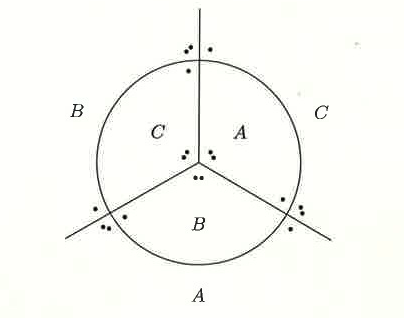
\includegraphics[scale=0.37]{images/diagram.png}
\end{center}
Bepaal de homologiegroepen van de bekomen ruimte.
\end{oef}


\section{Fixpuntstellingen}

Doordat we de homologie van de sfeer kennen, kunnen we nu ook voor hoger dimensionale
gesloten bollen de fixpuntstelling van Brouwer bewijzen.

\begin{stel} Zij $n\geq 1$. De rand $\Sf^{n-1}$ van de $n$-dimensionale bol $\D^n$ is geen retract van $\D^n$.
\label{retract}
\end{stel}
\bew Voor $n=1$ volgt de stelling uit het feit dat de rand van $\D^1=I$ niet samenhangend is.

Zij verder $n>1$. Onderstel dat $r:\D^n\to \Sf^{n - 1}$  een retract is. Door functorialiteit bekomen
we dat de afbeelding $H_{n-1}(r)\circ H_{n-1}(\iota):H_{n-1}(\Sf^{n-1})\to H_{n-1}(\Sf^{n-1})$ (met $\iota$ de canonische injectie van $\Sf^{n-1}$ in $\D^n$) gelijk is aan de identieke afbeelding.
Maar $H_{n-1}(\Sf^{n-1})\cong \Z$ en $H_{n-1}(\D^n)=0$ dus $H_{n-1}(\iota)$ en dan ook $H_{n-1}(r)\circ H_{n-1}(\iota)$ is de nulafbeelding. Een contradictie. \B

\begin{stel} (Brouwer Fixpuntstelling)
Een continue afbeelding van $\D^n$ naar zichzelf heeft een fixpunt.
\end{stel}
\bew Voor $n=0$ is de stelling triviaal. Voor $n=1$ volgt de stelling uit de tussenwaardestelling.

\textsc{Eerste Argument.}

Zij verder $n>1$. Onderstel dat $f:\D^n\to \D^n$ een continue afbeelding is zonder fixpunt. 
De rechte door de punten $x\in \D^n$ en $f(x)\in \D^n$ snijdt de sfeer $\Sf^{n-1}$ in twee punten, een punt $p_x$ ``aan de kant van $x$'' en een punt $p_{f(x)}$ ``aan de kant van $f(x)$''. De afbeelding die met $x$ het snijpunt $p_x$ associeert, definieert een retract van $\D^n\to \Sf^{n-1}$. Dit is in tegenspraak met Stelling~\ref{retract}. 

(Een vectori\"ele beschrijving van deze afbeelding laat toe de continu\"{\i}teit te verifi\"eren en  dus formeel te bewijzen dat de afbeelding weldegelijk een retract is.)


\textsc{Tweede Argument.}

We onderstellen dat $f$ geen fixpunt heeft. Dan is de afbeelding $F: \D^n \to \Sf^{n-1}:x\to \frac{x-f(x)}{|x-f(x)|}$ (met $x$ een element van de genormeerde vectorruimte $\R^n$) continu. We beweren dat de restrictie van deze afbeelding tot $\Sf^{n-1}$ homotoop is met de identiteit op $\Sf^{n-1}$. De homotopie wordt gegeven door $H(t,x):=\frac{x-tf(x)}{|x-tf(x)|}$. (Als $H$ niet continu is, bestaat er een $z\in \Sf^{n-1}$ zodat $z-tf(z)=0$. Uit $|z|=|t||f(z)|=1$ volgt dat $t=\frac{1}{|f(z)|}\geq 1$. Dit kan enkel als $t=1$, maar dan is $z=f(z)$ een fixpunt van $f$, wat tegen de onderstelling is.)

$H_{n-1}(F)$ is de nulafbeelding vermits $H_{n-1}(\D^{n})=0$, dus ook 
$$H_{n-1}(F_{\vert\Sf^{n-1}})=H_{n-1}(F)\circ H_{n-1}(\iota),$$
is de nulafbeelding. Maar 
$F_{|\Sf^{n-1}}$ en $\mbox{id}_{|\Sf^{n-1}}$ zijn homotoop, wat impliceert dat $H_{n-1}(\vert F_{\Sf^{n-1}})=H_{n-1}(\mbox{id}_{\vert\Sf^{n-1}})$. Dus de identieke afbeelding $H_{n-1}(\mbox{id}_{\vert\Sf^{n-1}})$ op $H_{n-1}(\Sf^{n-1})$ zou de nulafbeelding moeten zijn. Dit is een contradictie vermits $H_{n-1}(\Sf^{n-1})\cong \Z$. \B


%Om af te sluiten merken we op dat de De fixpunt stelling van Brouwer is maar \'e\'en van de vele fixpuntstelling uit de topologie. We geven nog een voorbeeld. Daarna formuleren we (zonder bewijs) een algemene fixpuntstelling waaruit de voorbeelden als speciale gevallen volgen.
%
%\begin{df} Zij $f:\Sf^{k}\to \Sf^{k}$ een continue afbeelding en $H_{k}(f):\Z\to \Z$ de ge\"{i}nduceerde afbeelding op de $k$-de homologiegroep. Dan defini\"eren we de {\em graad}\index{graad} van $f$ als $\deg f:=H_{k}(f)(1)$.
%\end{df}
%
%\begin{opm} De graad van de identiteit is gelijk aan 1. Dit volgt uit de functorialiteit van de homologie.
%
%De graad van de antipodale afbeelding (op $\Sf^k$) is gelijk aan $(-1)^{k+1}$. (We verwijzen naar Lemma 13.25 in J.Lee, Introduction to Topological Varieties, Springer, 2000.)
%\end{opm}
%
%\begin{stel} Zij $f:\Sf^{k}\to \Sf^{k}$ een continue afbeelding. Als $\deg f \not= (-1)^{k+1}$ dan heeft $f$ een fixpunt.
%\end{stel}
%
%\bew Als $f$ geen fixpunten heeft dan is $f$ homotoop met de antipodale afbeelding. De homotopie wordt gegeven door de continue familie $f_{t}(x)=\frac{tf(x)-(1-t)x}{|tf(x)-(1-t)x|}$. De continu\"{i}teit volgt uit het feit dat $tf(x)=(1-t)x$ impliceert dat $|t|=|t||f(x)|=|1-t||x|=|1-t|$. Dus $t=\frac{1}{2}$ maar dan is $f(x)=x$ wat in tegenspraak is met de onderstelling.
%
%Als $\deg f \not= (-1)^{k+1}$ dan is $f$ niet homotoop met de antipodale afbeelding; het voorgaande impliceert dat $f$ een fixpunt heeft. \B
%
%\bigskip
%Men kan aantonen dat alle homologiegroepen van compacte vari\"eteiten eindig voortgebrachte abelse groepen zijn. Verder geldt dat als $X$ een compacte vari\"eteit is van dimensie $n$, alle singuliere homologie groepen $H^m(X)$ met $m>n$ triviaal zijn.
%
%De hoofdstelling van de abelse groepen impliceert dat de homologiegroepen van een compacte vari\"eteit isomorf zijn
%met $\Z^n \oplus T$, waarbij $T$ een eindige groep is (de torsie-deelgroep). Vermits een morfisme van groepen 
%torsie-elementen op torsie-elementen afbeeldt, volgt dat elk morfisme van $\Z^n\oplus T \to \Z^n\oplus T$ een morfisme van
%$\Z^n \to \Z^n$ induceert. Zo een morfisme kunnen we voorstellen door een $n\times n$-matrix over $\Z$.
%
%Als $H_i(X)$, in het algemeen, een eindig voortgebrachte abelse groep is,  noteren we $\overline{H_{i}(X)}$ voor de groep $H_{i}(X)$ modulo de torsie deelgroep.
%
%\bigskip 
%Zij nu $X$ een compacte vari\"eteit. Een continue afbeelding $\varphi$ van $X$ naar zichzelf induceert dan 
%homomorfismen (door functorialiteit)
%
%$$\varphi_{i}:\overline{H_{i}(X)} \to \overline{H_{i}(X)}.$$ 
%
%Het spoor van $\varphi_{i}$, $\mbox{Tr}(\varphi)$, is het spoor van de matrix geassocieerd met $\varphi_i$. (Dit is goed gedefinieerd want het spoor van een matrix is invariant onder conjugatie.)
%
%\begin{df} Zij $X$ een compacte vari\"eteit en $\varphi$ een continue afbeelding van $X$ naar zichzelf. Dan is het {\em Lefschetz-getal}\index{Lefschetz-getal} van $\varphi$, genoteerd door $\tau(\varphi)$,  gelijk aan
%
%$$\tau(\varphi) = \sum_{i \geq 0} (-1)^{i}\mbox{Tr}(\varphi_{i}).$$
%
%Het Lefschetz-getal van de identiteit op $X$ is (per definitie) de Euler karakteristiek van $X$, i.e., $\chi(X):=\tau(\mbox{id}_{X})$.
%\end{df}
%
%\begin{stel} Zij $X$ een compacte vari\"eteit en $\varphi$ een continue afbeelding op $X$.
%
%Als het Lefschetz-getal $\tau(X)$ niet gelijk is aan nul, heeft $\varphi$ een fixpunt.
%\end{stel} 
%%Voor het bewijs van deze stelling zouden we de homologie theorie verder moeten ontwikkelen. Onder andere intersectie theorie %speelt een rol. Het is wel interessant om op te merken dat de fixpunt stellingen die we hiervoor
%%gegeven hebben speciale gevallen zijn van de fixpunt stelling van Lefschetz. 
%
%
%
%\section{De evenwichtsstelling van Nash}
%
%Fixpuntstellingen vormen een onderdeel van de topologie waarrond heel wat onderzoek verricht wordt. De toepassingen in de economie zijn hieraan zeker niet vreemd. De oorsprong van deze toepassingen ligt in de speltheorie (van von Neumann en Morgenstern) | meer bepaald in de ``evenwichtstelling van Nash''.
%
%We geven een korte uitzetting van deze stelling van Nash en volgen hierbij \'e\'en van de artikels van Nash over deze stelling.
%Ge\"{i}nteresseerden verwijzen we door naar de literatuur: The essential John Nash, edited by H.W. Kuhn and S. Nasar, Princeton University Press, 2002 - J.\ Milnor ``Nobel Prize for John Nash'', The Mathematical Intelligencer 17, nr. 3 (1995), p.11-17.
%
%\bigskip
%Een $n$-{\em persons game}\index{$n$-persons game} is een spel met $n$ spelers (of posities), $1\leq i \leq n$, en elke speler heeft 
%een eindige verzameling van (pure) {\em strategie\"en}\index{strategie\"en}, $\pi_{i, \alpha}$, $0\leq \alpha \leq m_i$. 
%
%Een  {\em mixed-strategie}\index{mixed-strategie} is een punt in een $m_i$-simplex waarvan de vertices de pure strategie\"en zijn, dus
%
%$$s_i=\sum_{\alpha} c_{i,\alpha}\pi_{i,\alpha}$$
%
%met $0\leq c_{i, \alpha} \leq 1, \sum_{\alpha} c_{i,\alpha}=1$ is een mixed-strategie voor speler $i$. (De $c_{i,\alpha}$ worden uniek bepaald door $s_i$.)
%
%We zeggen dat een mixed-strategie $s_i$ de strategie $\pi_{i, \alpha}$ gebruikt als $c_{i,\alpha} >0$.
%
%Een  ``strategie'' $S=(\pi_{1, \alpha_{1}}, \ldots , \pi_{n, \alpha_{n}})$ geeft elke speler een {\em payoff}\index{payoff}, een waarde in $\R$.
%Dus bij elke speler hoort een {\em payoff functie}\index{payoff functie}:
%
%$$p_{i}:(\pi_{1,\alpha_1}, \ldots , \pi_{n,\alpha_n}) \mapsto p_i(S) \in \R.$$
%
%Deze functie kan uitgebreid worden tot een functie van de mixed-strategie\"en (elementen in $\R^{m_{1}}\times \R^{m_{2}}\times \cdots \times \R^{m_{n}})$. De componentfuncties zijn functies op de $m_i$-simplexen. We nemen de gebruikelijke lineaire voortzetting, dus voor alle $i$ en alle $j$ geldt:
%
%$$p_i(\ldots, \sum_{\alpha} c_{j,\alpha}\pi_{j,\alpha}, \ldots )=\sum_{\alpha} c_{j,\alpha} p_i( \ldots , \pi_{j,\alpha}, \ldots ).$$
%
%Met ``strategie'' bedoelen we vanaf nu een $n$-tuppel $S=(s_1, \ldots , s_n)$ (van mixed-strategie\"en) in $\Delta_{m_{1}} \times \cdots \times \Delta_{m_{n}}$. Als enkel speler $i$ zijn strategie wijzigt van $s_i$ naar $t_i$, noteren we dit met 
%
%$$(S; t_i)=(s_1, \ldots, s_{i-1}, t_i, s_{i+1}, \ldots , s_n).$$
%
%\begin{df}
%Een strategie $S$ heet een  {\em evenwichtspunt}\index{evenwichtspunt} als voor alle spelers $i$, 
%
%$$p_{i}(S)=\max_{r_i}[p_i(S;r_i)].$$ 
%
%Dus elke speler maximaliseert met  ``zijn strategie'' $s_i$ (van de strategie $S$) zijn payoff als de andere spelers hun strategie niet wijzigen. 
%\end{df}
%
%Vermits $p_i$ lineair is in $s_i$ volgt voor een evenwichtspunt $S$ dat
%
%$$p_{i}(S)=\max_{r_i}\{p_i(S;r_i)\}=\max_{\alpha}\{p_i(S;\pi_{i, \alpha})\}.$$
%
%Namelijk 
%
%\begin{eqnarray*}
%p_i(S,r_i)& = &p_i(\ldots, \sum_{\beta} c_{i,\beta} \pi_{i, \beta}, \ldots )\\
%& = & \sum_{\beta} c_{i,\beta} p_{i}(\ldots , \pi_{i, \beta}, \ldots )\\
%& \leq  & \max_{\alpha} p_{i}(\ldots , \pi_{i, \alpha}, \ldots ).\end{eqnarray*}
%
%(De ongelijkheid volgt uit het feit dat $\sum_{\alpha} c_{i,\alpha}=1$.)
%
%Dus $S$ is een evenwichtspunt als en slechts als $p_i(S)=\max_{\alpha} \{p_{i}(S, \pi_{i,\alpha})\}$.
%
%Noteren we eenvoudigheidshalve $p_{i, \alpha}(S):=p_{i}(S, \pi_{i,\alpha})$. We zien dat als $p_i(S)=\max_{\alpha} p_{i, \alpha}(S)$, noodzakelijk $c_{i,\gamma}=0$ als $p_{i,\gamma}(S)< \max_{\alpha} p_{i,\alpha}(S).$ (Anders is $p_i(S)=
%\sum c_{i,\alpha}p_{i,\alpha}(S) <\max_{\alpha} p_{i,\alpha}(S)$.)
%
%Dus in een evenwichtsstrategie $S$ gebruikt speler $i$ enkel $\pi_{i,\alpha}$ als $\pi_{i, \alpha}$ een optimale strategie is voor $i$. (Optimaal als de andere spelers hun strategie vast ligt.)
%
%Een nodige en voldoende voorwaarde omdat $S$ een evenwichtspunt zou zijn is dus: als 
%$s_i$ de strategie $\pi_{i,\alpha}$ gebruikt, dan is $p_{i,\alpha}(S)=\max _{\beta} p_{i,\beta}(S).$
%
%\begin{stel} (Nash Evenwichtsstelling)
%
%Elk spel heeft een evenwichtspunt.
%\end{stel}
%
%\bew Met de notaties zoals hiervoor defini\"eren we
%
%$$\varphi_{i,\alpha}(S)=\max(0, p_{i,\alpha}(S)-p_i(S))$$
%
%Merk op dat de $\varphi_{i,\alpha}$ continu zijn in $S$.
%
%Elke component $s_i$ modifi\"eren we als volgt:
%
%$$s_{i}'=\frac{s_i+\sum_{\alpha} \varphi_{i,\alpha}(S)\pi_{i,\alpha}}{1+\sum_{\alpha}\varphi_{i,\alpha}(S)}.$$
%
%Deze $s_{i}'$ is een mixed-strategie voor $i$. Namelijk
%
%$$s_{i}'= \frac{\sum_{\alpha} c_{i,\alpha}\pi_{i,\alpha}+\sum_{\alpha} \varphi_{i,\alpha}(S)\pi_{i,\alpha}}{1+\sum_{\alpha}\varphi_{i,\alpha}(S)}=
%\sum_{\alpha}\frac{c_{i,\alpha}+ \varphi_{i,\alpha}(S)}{1+\sum_{\alpha}\varphi_{i,\alpha}(S)}\pi_{i,\alpha},$$
%
%met 
%
%$$ 0\leq \frac{c_{i,\alpha}+ \varphi_{i,\alpha}(S)}{1+\sum_{\alpha}\varphi_{i,\alpha}(S)}\leq 1\ \ \mbox{en}\ \ \frac{1}{1+\sum_{\alpha}\varphi_{i,\alpha}(S)}(\sum_{\alpha}c_{i,\alpha}+ \varphi_{i,\alpha}(S))=1.$$
%
%Dus $T:\Delta_{m_{1}}\times \cdots \times \Delta_{m_{n}}\to \Delta_{m_{1}}\times \cdots \times \Delta_{m_{n}}: (s_1, \ldots , s_n)\mapsto (s_{1}', \ldots , s_{n}')$ is een continue functie.
%Vermits $\Delta_{m_{1}}\times \cdots \times \Delta_{m_{n}}$ homeomorf is met een $(m_1+\cdots +m_n)$-dimensionale
%gesloten bol, heeft $T$ een fixpunt vanwege de fixpuntstelling van Brouwer.
%
%Zij $S=(s_1, \ldots , s_n)$ een fixpunt voor $T$, met $s_i=\sum_{\alpha} c_{i,\alpha}\pi_{i,\alpha}$. 
%
%Als alle strategie\"en die $s_i$ gebruikt optimaal zijn, i.e., $p_{i,\alpha}(S)=\max_{\beta}p_{i,\beta}(S)$, is de stelling bewezen want dan is $S$ een evenwichtspunt. Zij $\pi_{i,\alpha}$ een strategie waarvoor $p_{i,\alpha}(S)<\max_{\beta}p_{i,\beta}(S)$, en kies $\alpha$ zodat $p_{i, \alpha}(S)$ minimaal is. Dan is 
%$$p_{i,\alpha}(S)=(\sum c_{i,\beta})p_{i,\alpha}(S)\leq \sum c_{i,\beta}p_{i,\beta}(S)=p_{i}(S).$$
%Dit impliceert dat $\varphi_{i,\alpha}(S)=0$.
%
%Vermits $S$ een fixpunt is van $T$, dus $S'=T(S)=S$, volgt dat
%$$c_{i,\alpha}=\frac{c_{i,\alpha}}{1+\sum_{\beta} \varphi_{i,\beta}(S)}=c_{i,\alpha}'.$$
%Maar dan moet $\varphi_{i,\beta}(S)=0$ voor alle $\beta$. Dus $p_{i,\beta}\leq p_{i}(S)$ voor alle $\beta$. 
%
%De speler kan dus zijn payoff niet verhogen door {\em zijn} strategie te wijzigen: $S$ is dus een evenwichtspunt. \B
%
%
% \begin{opm}
%Omgekeerd zien we onmiddellijk dat een evenwichtspunt voor het spel ook een fixpunt voor de afbeelding $T$ is. In een evenwichtspunt verdwijnen immers per definitie alle $\varphi_{i,\alpha}$.
%\end{opm}
%
%   
%
% 
%
%     



  


%\newpage
%\input{oefdeel3}
%\input{oploef}
%\input{deel5}
%\printindex

\chapter{Vrije groepen}

In dit hoofdstuk bestuderen we de vrije groep $F_n := \langle x_1, \dots , x_n \rangle$ op $n$ generatoren. Onze aanpak zal deels met combinatorische technieken zijn, en deels met topologische technieken, in het bijzonder homotopietheorie.

We zullen aantonen dat de deelgroepen van $F_n$ opnieuw vrije groepen zijn, en de automorfismegroep van de vrije groep bespreken.

\section{Grafen en vrije groepen}

De topologische ruimten die we beschouwen in dit hoofdstuk zijn (multi)grafen $\Gamma$ met verzameling toppen $V(\Gamma)$ en verzameling bogen $E(\Gamma)$. Men kan deze als topologische ruimte beschouwen door ze op te vatten als CW-complexen bestaande uit 0- en 1-cellen.

De afbeeldingen tussen grafen die we zullen beschouwen zullen (combinatorische) graafmorfismes zijn. Merk op dat een graafmorfisme automatisch continu is.

\begin{df}
Een graaf is een \emph{boom} als deze geen cykels bevat en samenhangend is. Een \emph{opspannende boom} $T$ van een graaf $\Gamma$ is een deelgraaf van $\Gamma$ die alle toppen van $\Gamma$ bevat, en een boom is.
\end{df}

\begin{lem}
Elke samenhangende graaf $\Gamma$ heeft een opspannende boom als deelgraaf.
\end{lem}
\bew
Beschouw de verzameling $K$ van deelgrafen van $\Gamma$ die geen cykels bevatten. De verzameling $K$ kunnen we partieel ordenen door inclusie. Aangezien elke totaal geordende deelverzameling van $K$ een bovengrens heeft (namelijk de unie van al de grafen in deze deelverzameling), kunnen we het Lemma van Zorn toepassen en besluiten dat $K$ een bovengrens $T$ heeft. 

Veronderstel dat $T$ niet alle toppen van $\Gamma$ aandoet. Dan bestaat er, wegens de samenhang\-endheid van $\Gamma$, een top $v$ in $T$ adjacent (in $\Gamma$) met een top $w$ niet bevat in $T$. Hierdoor zouden we $T$ kunnen uitbreiden met een boog tussen $v$ en $w$, wat ons grotere bovengrens zou opleveren. Een tegenstrijdigheid.

Analoog bewijst men dat $T$ samenhangend is. We concluderen dat $T$ een opspannende boom is.
\B




We lijsten nu enkele eenvoudige resultaten op.

\begin{lem}
Elk zelf-homeomorfisme van een graaf is homotoop met een graafautomorfisme.
\end{lem}

\begin{lem}
Het quoti\"ent van een graaf onder een groep van graafautomorfismes is opnieuw een graaf.
\end{lem}

%\begin{lem}
%Elk pad in een graaf is homotoop met 


\subsection{De fundamentaalgroep van een graaf}

Voor het boeket $R_n$  op $n$ cirkels hadden we de fundamentaalgroep reeds berekend. Namelijk als $x_0$ het vertakkingspunt is in $R_n$, dan was de fundamentaalgroep $\pi_1(R_n,x_0)$ van het boeket isomorf met de vrije groep $F_n$, waarbij een natuurlijke keuze voor de generatoren de (geori\"enteerde) cirkels $l_1, \dots, l_n$ van het boeket zijn door $x_0$.

%
%Centraal zal het boeket met $n$ cirkels staan, deze topologische ruimte noteren we met $R_n$. Zij $x_0$ het vertakkingspunt in $R_n$, dan is de fundamentaalgroep $\pi_1(R_n,x_0)$ van het boeket isomorf met de vrije groep $F_n$, waarbij een natuurlijke keuze voor de generatoren de (geori\"enteerde) cirkels $l_1, \dots, l_n$ van het boeket zijn door $x_0$.

We bewijzen nu een meer algemeen resultaat voor algemene grafen.

\begin{lem}\label{fungra}
De fundamentaalgroep $\pi_1(\Gamma, x_0)$ van een samenhangende graaf $\Gamma$ is isomorf met de vrije groep $F_n$, waarbij $n$ het aantal bogen is niet bevat in een gekozen opspannende boom $T$ die $x_0$ bevat.
\end{lem}
\bew
Het bewijs hiervan is volledig analoog aan het bewijs voor het boeket $R_n$ op $n$ cirkels. Men neemt een open samentrekbare uitbreiding $U$ van de opspannende boom $T$, en als open overdekking van $\Gamma$ nemen we de unies van bogen niet bevat in $T$ met $U$. \B

\begin{gev}\label{numbergen}
De fundamentaalgroep $\pi_1(\Gamma, x_0)$ van een samenhangende graaf $\Gamma$ is isomorf met de vrije groep $F_n$, waarbij $n = E(\Gamma) - V(\Gamma) + 1$.
\end{gev}
\bew
Dit volgt uit het feit dat het aantal bogen in een boom gelijk is aan het aantal toppen min \'e\'en.
\B


\subsection{De Cayley-graaf van een vrije groep}

We starten met een definitie.
\begin{df}
Een groep $G$ van graafautomorfismes van een graaf $\Gamma$ werkt \emph{vrij} als geen enkel niet-triviaal element van $G$ toppen fixeert of bogen stabiliseert.
\end{df}

Het doel van deze sectie is om aan te tonen dat een vrije groep $F_n$ vrij werkt op een boom. In de volgende sectie zal blijken dat dit vrije groepen karakteriseert.

\begin{df}
Zij $G$ een groep voorgebracht door een verzameling elementen $S$. Dan is de \emph{Cayley-graaf} $\mathsf{Cay}(G,S)$ van $G$ ten opzichte van $S$ de enkelvoudige graaf gevormd door de toppen $v_g$, met $g \in G$ (dus voor elk element van $G$ een top), waarbij de toppen $v_g$ en $v_h$ adjacent zijn als $g^{-1}h$ bevat is in $S$ of $S^{-1}$. 
\end{df}

Vaak ori\"enteert en labelt men bogen van de graaf voor de duidelijkheid. 

\begin{vb}
Hieronder is een deel van de Cayley-graaf van de vrije groep op 2 generatoren $a$ en $b$ weergegeven.

\begin{center}
\begin{tikzpicture}
\draw[->-=.5] (0,0) -- node [above] {$a$} (2,0);
\draw[->-=.5] (-2,0) -- node [above] {$a$} (0,0);
\draw[->-=.5] (-3.2,0) -- node [above] {$a$} (-2,0);
\draw[->-=.5] (2,0) -- node [above] {$a$} (3.2,0);

\draw[->-=.5] (-1.2,2) -- node [above] {$a$} (0,2);
\draw[->-=.5] (0,2) -- node [above] {$a$} (1.2,2);

\draw[->-=.5] (-1.2,-2) -- node [above] {$a$} (0, -2);
\draw[->-=.5] (0,-2) -- node [above] {$a$} (1.2,-2);

\draw[->-=.5] (0,0) -- node [right] {$b$} (0,2);
\draw[->-=.5] (0,-2) -- node [right] {$b$} (0,0);
\draw[->-=.5] (0,-3.2) -- node [right] {$b$} (0,-2);
\draw[->-=.5] (0,2) -- node [right] {$b$} (0,3.2);


\draw[->-=.5] (-2,0) -- node [right] {$b$} (-2,1.2);
\draw[->-=.5] (-2,-1.2) -- node [right] {$b$} (-2,0);

\draw[->-=.5] (2,0) -- node [right] {$b$} (2,1.2);
\draw[->-=.5] (2,-1.2) -- node [right] {$b$} (2,0);

%\fill[fill=LGray] (0,0) -- (2,0) -- (2,2) -- (0,2) -- (0,0);
%\draw[->-=.5] (0,0) -- node [below] {$b$} (2,0); 
%\draw[->-=.5] (0,2) -- node [above] {$b$} (2,2); 
%\draw[->-=.5] (0,0) -- node [left] {$a$} (0,2); 
%\draw[->-=.5] (2,0) -- node [right] {$a$} (2,2); 
\end{tikzpicture}
\end{center}
\end{vb}


We kunnen groepselementen $h \in G$ laten inwerken op $\mathsf{Cay}(G,S)$ als volgt: $v_g \mapsto v_{hg}$. Men gaat eenvoudig na dat dit adjacentie bewaart, waardoor $G$ beschouwd kan worden als een deelgroep van de graafautomorfismegroep van $\mathsf{Cay}(G,S)$. Deze actie is scherp-transitief op de toppen.


\begin{stel}
Zij $F_n := \langle x_1, \dots , x_n \rangle$ de vrije groep op $n$ generatoren, dan is de Cayley-graaf $\mathsf{Cay}(F_n,\{x_1, \dots, x_n\})$ een boom.
\end{stel}
\bew
We noteren de graaf $\mathsf{Cay}(F_n,\{x_1, \dots, x_n\})$ kortweg door $\Gamma$. Aangezien $x_1, \dots, x_n$ de vrije groep genereren volgt er dat $\Gamma$ samenhangend is. Veronderstel nu dat toppen $v_{h_0}, v_{h_1}, \dots, v_{h_m} = v_{h_0}$ een  minimale cykel in $\Gamma$ vormen. Per definitie van de Cayley-graaf zijn de elementen ${h_0}^{-1} h_1, \dots, {h_{m-1}}^{-1} h_m$ letters $s_1, \dots, s_m$ in $ \{x_1, x_1^{-1}, \dots, x_n,  x_n^{-1}\}$. 

Het woord $s_1\dots s_m$ zou nu het triviaal element moeten representeren, wat inhoudt dat er een $i$ is in $\{1, \dots m-1\}$ zodanig dat $s_i^{-1} = s_{i+1}$. Dit zou echter impliceren dat de toppen $v_{h_{i-1}}$ en $v_{h_{i+1}}$ identiek zijn, wat onmogelijk is voor een minimale cykel in een enkelvoudige graaf. \B

\subsection{Vrije acties op bomen}

Het volgende lemma karakteriseert vrije acties op bomen.

\begin{lem}
Als een groep $G$ vrij werkt op een boom, dan is $G$ een vrije groep.
\end{lem}
\bew
Zo een actie van de groep $G$ op de topologische ruimte gevormd door $T$ voldoet aan de eigenschappen vermeld op pagina~\pageref{freeaction}. Er volgt dat de groep $G$ isomorf is aan de fundamentaalgroep van de quoti\"entruimte bekomen uit $T$ door de banen van $G$ te identificeren. Deze quoti\"entruimte is een graaf, dus is $G$ een vrije groep.
\B

\begin{stel}\textbf{\em(Nielsen-Schreier)}
Elke deelgroep $H$ van een vrije groep $F_n$ is opnieuw een vrije groep. Indien $H$ eindige index $m$ heeft in $F_n$, dan is $H$ isomorf aan $F_{mn - m + 1}$.
\end{stel}
\bew
De groep $F_n$ werkt vrij op zijn Cayley-graaf $\mathsf{Cay}(F_n,\{ x_1, \dots , x_n \})$, wat een $2n$-reguliere boom is. Een deelgroep $H$ werkt ook vrij op deze graaf, dus er volgt dat $H$ een vrije groep is.

Veronderstel nu dat $[F_n: H] = m < \infty$.  Aangezien $F_n$ scherp-transitief werkt op de toppen, heeft de deelgroep $m$ banen op de toppen. De graaf bekomen als quoti\"ent van $\mathsf{Cay}(F_n,\{ x_1, \dots , x_n \})$ door $H$ heeft dus $m$ toppen en is $2n$-regulier. Uit een dubbele telling halen we het aantal bogen in dit quoti\"ent, namelijk $mn$. Door Gevolg~\ref{numbergen} hebben we nu dat $H$ isomorf is met $F_{mn - m + 1}$. \B

We merken op dat een vrije groep $F_n$ deelgroepen bevat isomorf aan $F_m$ waarbij $m$ willekeurig hoog is, zelfs oneindig. In het bijzonder dat een eindig gegenereerde groep oneindig gegenereerde deelgroepen kan bevatten.


\section{De automorfismegroep $\mathrm{Aut}(F_n)$}

Ons volgend doel is de automorfismegroep van de vrije groep $F_n$ te bestuderen. We starten met enkele eenvoudige automorfismes te beschouwen. Het volstaat steeds om het beeld van de generatoren $x_1, \dots, x_n$ te specifi\"eren. 
 
Een eerste mogelijkheid zijn transposities van generatoren $x_1, \dots, x_n$, een tweede is het omwisselen van $x_i$ met $x_i^{-1}$ voor een zekere $i$. Een derde mogelijkheid wordt gegeven door de volgende beelden van de generatoren.
\begin{align*}
x_1 & \mapsto x_1 x_2 \\
x_2 & \mapsto x_2 \\
&\dots  \\
x_n &\mapsto x_n
\end{align*}

Deze verschillende generatoren noemt men \emph{Nielsen-generatoren}.

Het doel van de komende secties is een algoritme op te stellen dat na gaat wanneer een bepaald endomorfisme van de vrije groep (gegeven door de beelden van de generatoren), een automorfisme is. Dit zullen we doen met behulp van Stallingsvouwen.
%Vooraleer we automorfismes van vrije groepen in detail bekijken voeren we eerst het begrip Stallingsvouwen in.

\begin{oef}\label{Niel}
Men kan automorfismes ook opvatten als het nemen van een andere keuze van generatoren. Toon aan dat de automorfismes die men bekomt door in Lemma~\ref{fungra} een andere opspannende boom te kiezen gegenereerd worden door Nielsen-generatoren. Hint: verander de opspannende boom stap per stap.
\end{oef}



\subsection{Stallingsvouwen}

\begin{df} 
Een \emph{geori\"enteerde boog} van een graaf is een boog waarbij we een onderscheid maken tussen beginpunt en eindpunt. Het beginpunt van een geori\"enteerde boog $\vec{e}$ noteren we met $o(\vec{e})$, het eindpunt met $t(\vec{e})$.
\end{df}

\begin{df}
Een graafmorfisme $f:\Gamma \to \Delta$ is \emph{lokaal injectief} als er geen twee geori\"enteerde bogen $\vec{d}$ en $\vec{e}$ met zelfde beginpunt bestaan waarbij $f(\vec{d}) = f(\vec{e})$.
\end{df}

\begin{df}
Zij $\Gamma$ en $\Delta$ twee grafen, dan is een \emph{Stallingsvouw} (of kortweg \emph{vouw}) een continue quoti\"entafbeelding $$f_{\vec{d}, \vec{e}} \colon \Gamma \to \Delta$$
die twee geori\"enteerde bogen $\vec{d}$ en $\vec{e}$ met zelfde beginpunt identificeert. De vouw is \emph{singulier} als $t(\vec{d}) = t(\vec{e})$, en \emph{niet-singulier} in het andere geval.
\end{df}

Hierbij kunnen we direct opmerken dat een niet-singuliere vouw een homotopie-equivalentie is, en dus een isomorfisme ${f_{\vec{d}, \vec{e}}}_* \colon \pi_1(\Gamma, x) \to \pi_1(\Delta, f_{\vec{d}, \vec{e}}(x))$ induceert. Een singuliere vouw zal daarentegen een niet-injectieve afbeelding op de homotopiegroepen induceren.


\begin{lem}\label{lem:step1}
Zij $\phi\colon \Gamma \to \Delta$ een graafmorfisme dat niet lokaal injectief is. Dan is er een vouw $f$ zodanig dat $\phi$ factoriseert in graafmorfismen als $\phi' \circ f$.
\end{lem}
\bew
Rechtstreeks uit de definitie van lokaal injectief. \B

\begin{stel}\label{stel:fact}
Zij $\Gamma$ een eindige graaf, en $\phi: \Gamma \to \Delta$ een graafmorfisme, dan is er een eindige factorisatie 
$$\Gamma = \Gamma_0  \overset{f_1}{\to} \Gamma_1 \overset{f_2}{\to} \dots \overset{f_r}{\to}  \Gamma_r \overset{\psi}{\to} \Delta $$ van $\phi$ waarbij de $f_i$ vouwen zijn, en $\psi$ een lokaal injectief graafmorfisme.
\end{stel}
\bew
We passen Lemma~\ref{lem:step1} herhaaldelijk toe, we kunnen dit slechts een eindig aantal keer doen aangezien dit het aantal bogen vermindert. Het resulterende graafmorfisme is dan noodzakelijkerwijs lokaal injectief.
\B

\subsection{Endomorfismes van de vrije groep}

Zij $\alpha$ een automorfisme van de vrije groep $F_n := \langle x_1, \dots , x_n \rangle$. Om $\alpha$ voor te stellen volstaat het de beelden van de generators te kennen, stel $w_i := \alpha(x_i)$.

We construeren nu een graaf $\overline{R_n}$ uit $R_n$ als volgt. We doen dit door de lus $l_i$ op te delen in $l(w_i)$ bogen ($l(w_i)$ is de lengte van een gereduceerd woord voor het element $w_i$). Als topologische ruimte is $\overline{R_n}$ homeomorf met $R_n$.

Door de lus $l_i$ in $\overline{R_n}$ af te beelden op de opeenvolging van lussen (rekening houdend met de orientatie) in een gereduceerd woord voor $w_i$ bekomen we een graafmorfisme $\phi : \overline{R_n} \to R_n$.

Het ge\"induceerde morfisme $\pi_1(\phi)  \colon \pi_1(\overline{R_n},x_0) \to \pi_1(R_n,x_0)$ is, na gebruik makend van het standaardisomorfisme van $F_n$ met $\pi_1(\overline{R_n},x_0)$ en $\pi_1(R_n,x_0)$, precies het endomorfisme $\alpha$. Men kan dit inzien door de beelden van de generators $x_i$ te bekijken.

We factoriseren nu $\phi$ als in Stelling~\ref{stel:fact}, we hebben dus 
$$
\phi = \psi \circ f_r \circ \dots f_1
$$
waarbij de $f_i$ vouwen zijn en $\psi\colon \Gamma_r \to \Delta$ lokaal injectief. De vouwen $f_i$ zijn noodzakelijkerwijs niet-singulier, anders zou $\phi_*$ geen een isomorfisme kunnen zijn.

\begin{lem}
Het graafmorfisme $\psi$ is een isomorfisme.
\end{lem}
\bew
We weten reeds dat $\psi$ lokaal injectief is. Ook weten we dat $\psi$ surjectief is, aangezien $\phi$ dit is. Kies een top $y$ van $\Gamma_r$ die op $x_0$ wordt afgebeeld. Aangezien $\psi_*\colon \pi_1(\Gamma_r,y) \to \pi_1(\Delta,x_0)$ een isomorfisme is, bestaat er voor elke lus $l_i$ van $R_n$ een lus $p_i$ van $\Gamma_r$ met basispunt $y$.

We kunnen veronderstellen dat $p_i$ een pad in de graaf is zonder terugkeren, aangezien $\psi$ lokaal injectief is zal het beeld van dit pad ook zonder terugkeren zijn. Merk nu op dat het enige pad zonder terugkeren in $\Delta$ met begin- en eindpunt $x_0$ homotoop met $l_i$ is $l_i$ zelf.

Hieruit concluderen we dat er voor elke lus $l_i$ een unieke lus $p_i$ is met basispunt $y$ is die op $l_i$ wordt afgebeeld. Uit lokaal injectiviteit halen we tenslotte dat deze lussen de volledige graaf $\Gamma_r$ vormen en dat $\psi$ een isomorfisme is.
\B

Dit heeft nu het volgende gevolg, wat ons toe laat automorfismes te herkennen.

\begin{stel}
Een toewijzing $x_i \to w_i$ genereert een automorfisme van $F_n$ als en slechts als het ge\"induceerd graafmorfisme factoriseert als $$\phi = \psi \circ f_r \circ \dots f_1,$$ waarbij $\psi$ een isomorfisme is en de $f_i$ niet-singuliere vouwen.
\end{stel}
\bew
Indien $\phi$ een automorfisme is volgt uit het voorgaande dat er zo een factorisatie is. Stel nu dat er zo een factorisatie bestaat. Aangezien elke stap een homotopie-equivalentie is, zal er op niveau van de homotopiegroepen een isomorfisme optreden.
\B

\begin{oef}
Toon aan dat $\mathrm{Aut}(F_n)$ gegenereerd wordt door Nielsen-generatoren. Hint: maak gebruik van het voorgaande en Oefening~\ref{Niel}.
\end{oef}

\end{document}


